\documentclass[]{book}
\usepackage{lmodern}
\usepackage{amssymb,amsmath}
\usepackage{ifxetex,ifluatex}
\usepackage{fixltx2e} % provides \textsubscript
\ifnum 0\ifxetex 1\fi\ifluatex 1\fi=0 % if pdftex
  \usepackage[T1]{fontenc}
  \usepackage[utf8]{inputenc}
\else % if luatex or xelatex
  \ifxetex
    \usepackage{mathspec}
  \else
    \usepackage{fontspec}
  \fi
  \defaultfontfeatures{Ligatures=TeX,Scale=MatchLowercase}
\fi
% use upquote if available, for straight quotes in verbatim environments
\IfFileExists{upquote.sty}{\usepackage{upquote}}{}
% use microtype if available
\IfFileExists{microtype.sty}{%
\usepackage{microtype}
\UseMicrotypeSet[protrusion]{basicmath} % disable protrusion for tt fonts
}{}
\usepackage{hyperref}
\hypersetup{unicode=true,
            pdftitle={The Book of OHDSI},
            pdfauthor={Observational Health Data Science and Informatics},
            pdfborder={0 0 0},
            breaklinks=true}
\urlstyle{same}  % don't use monospace font for urls
\usepackage{natbib}
\bibliographystyle{apalike}
\usepackage{color}
\usepackage{fancyvrb}
\newcommand{\VerbBar}{|}
\newcommand{\VERB}{\Verb[commandchars=\\\{\}]}
\DefineVerbatimEnvironment{Highlighting}{Verbatim}{commandchars=\\\{\}}
% Add ',fontsize=\small' for more characters per line
\usepackage{framed}
\definecolor{shadecolor}{RGB}{248,248,248}
\newenvironment{Shaded}{\begin{snugshade}}{\end{snugshade}}
\newcommand{\KeywordTok}[1]{\textcolor[rgb]{0.13,0.29,0.53}{\textbf{#1}}}
\newcommand{\DataTypeTok}[1]{\textcolor[rgb]{0.13,0.29,0.53}{#1}}
\newcommand{\DecValTok}[1]{\textcolor[rgb]{0.00,0.00,0.81}{#1}}
\newcommand{\BaseNTok}[1]{\textcolor[rgb]{0.00,0.00,0.81}{#1}}
\newcommand{\FloatTok}[1]{\textcolor[rgb]{0.00,0.00,0.81}{#1}}
\newcommand{\ConstantTok}[1]{\textcolor[rgb]{0.00,0.00,0.00}{#1}}
\newcommand{\CharTok}[1]{\textcolor[rgb]{0.31,0.60,0.02}{#1}}
\newcommand{\SpecialCharTok}[1]{\textcolor[rgb]{0.00,0.00,0.00}{#1}}
\newcommand{\StringTok}[1]{\textcolor[rgb]{0.31,0.60,0.02}{#1}}
\newcommand{\VerbatimStringTok}[1]{\textcolor[rgb]{0.31,0.60,0.02}{#1}}
\newcommand{\SpecialStringTok}[1]{\textcolor[rgb]{0.31,0.60,0.02}{#1}}
\newcommand{\ImportTok}[1]{#1}
\newcommand{\CommentTok}[1]{\textcolor[rgb]{0.56,0.35,0.01}{\textit{#1}}}
\newcommand{\DocumentationTok}[1]{\textcolor[rgb]{0.56,0.35,0.01}{\textbf{\textit{#1}}}}
\newcommand{\AnnotationTok}[1]{\textcolor[rgb]{0.56,0.35,0.01}{\textbf{\textit{#1}}}}
\newcommand{\CommentVarTok}[1]{\textcolor[rgb]{0.56,0.35,0.01}{\textbf{\textit{#1}}}}
\newcommand{\OtherTok}[1]{\textcolor[rgb]{0.56,0.35,0.01}{#1}}
\newcommand{\FunctionTok}[1]{\textcolor[rgb]{0.00,0.00,0.00}{#1}}
\newcommand{\VariableTok}[1]{\textcolor[rgb]{0.00,0.00,0.00}{#1}}
\newcommand{\ControlFlowTok}[1]{\textcolor[rgb]{0.13,0.29,0.53}{\textbf{#1}}}
\newcommand{\OperatorTok}[1]{\textcolor[rgb]{0.81,0.36,0.00}{\textbf{#1}}}
\newcommand{\BuiltInTok}[1]{#1}
\newcommand{\ExtensionTok}[1]{#1}
\newcommand{\PreprocessorTok}[1]{\textcolor[rgb]{0.56,0.35,0.01}{\textit{#1}}}
\newcommand{\AttributeTok}[1]{\textcolor[rgb]{0.77,0.63,0.00}{#1}}
\newcommand{\RegionMarkerTok}[1]{#1}
\newcommand{\InformationTok}[1]{\textcolor[rgb]{0.56,0.35,0.01}{\textbf{\textit{#1}}}}
\newcommand{\WarningTok}[1]{\textcolor[rgb]{0.56,0.35,0.01}{\textbf{\textit{#1}}}}
\newcommand{\AlertTok}[1]{\textcolor[rgb]{0.94,0.16,0.16}{#1}}
\newcommand{\ErrorTok}[1]{\textcolor[rgb]{0.64,0.00,0.00}{\textbf{#1}}}
\newcommand{\NormalTok}[1]{#1}
\usepackage{longtable,booktabs}
\usepackage{graphicx,grffile}
\makeatletter
\def\maxwidth{\ifdim\Gin@nat@width>\linewidth\linewidth\else\Gin@nat@width\fi}
\def\maxheight{\ifdim\Gin@nat@height>\textheight\textheight\else\Gin@nat@height\fi}
\makeatother
% Scale images if necessary, so that they will not overflow the page
% margins by default, and it is still possible to overwrite the defaults
% using explicit options in \includegraphics[width, height, ...]{}
\setkeys{Gin}{width=\maxwidth,height=\maxheight,keepaspectratio}
\IfFileExists{parskip.sty}{%
\usepackage{parskip}
}{% else
\setlength{\parindent}{0pt}
\setlength{\parskip}{6pt plus 2pt minus 1pt}
}
\setlength{\emergencystretch}{3em}  % prevent overfull lines
\providecommand{\tightlist}{%
  \setlength{\itemsep}{0pt}\setlength{\parskip}{0pt}}
\setcounter{secnumdepth}{5}
% Redefines (sub)paragraphs to behave more like sections
\ifx\paragraph\undefined\else
\let\oldparagraph\paragraph
\renewcommand{\paragraph}[1]{\oldparagraph{#1}\mbox{}}
\fi
\ifx\subparagraph\undefined\else
\let\oldsubparagraph\subparagraph
\renewcommand{\subparagraph}[1]{\oldsubparagraph{#1}\mbox{}}
\fi

%%% Use protect on footnotes to avoid problems with footnotes in titles
\let\rmarkdownfootnote\footnote%
\def\footnote{\protect\rmarkdownfootnote}

%%% Change title format to be more compact
\usepackage{titling}

% Create subtitle command for use in maketitle
\providecommand{\subtitle}[1]{
  \posttitle{
    \begin{center}\large#1\end{center}
    }
}

\setlength{\droptitle}{-2em}

  \title{The Book of OHDSI}
    \pretitle{\vspace{\droptitle}\centering\huge}
  \posttitle{\par}
    \author{Observational Health Data Science and Informatics}
    \preauthor{\centering\large\emph}
  \postauthor{\par}
      \predate{\centering\large\emph}
  \postdate{\par}
    \date{2019-06-01}

\usepackage{booktabs}
\usepackage{amsthm}
\makeatletter
\def\thm@space@setup{%
  \thm@preskip=8pt plus 2pt minus 4pt
  \thm@postskip=\thm@preskip
}
\makeatother

\begin{document}
\maketitle

{
\setcounter{tocdepth}{1}
\tableofcontents
}
\chapter*{Preface}\label{preface}
\addcontentsline{toc}{chapter}{Preface}

 This is a book about OHDSI, and is currently very much under
development.

The book is written in \href{https://rmarkdown.rstudio.com}{RMarkdown}
with \href{https://bookdown.org}{bookdown}. It is automatically rebuilt
from \href{https://github.com/OHDSI/TheBookOfOhdsi}{source} by
\href{http://travis-ci.org/}{travis}.

\section*{Goals of this book}\label{goals-of-this-book}
\addcontentsline{toc}{section}{Goals of this book}

This book aims to be a central knowledge repository for OHDSI, and
focuses on describing the OHDSI community, data standards, and tools. It
is intended both for those new to OHDSI and veterans alike, and aims to
be practical, providing the necessary theory and subsequent instructions
on how to do things. After reading this book you will understand what
OHDSI is, and how you can join the journey. You will learn what the
common data model and standard vocabularies are, and how they can be
used to standard an observational healthcare database. You will learn
there are three main uses cases for these data: characterization,
population-level estimation, and patient-level prediction, and that all
three activities are supported by OHDSI's open source tools, and how to
use them. You will learn how to establish the quality of the generated
evidence through data quality, clinical validity, software validity, and
method validity. Lastly, you will learn how these tools can be used to
execute these studies in a distributed research network.

\section*{Structure of the book}\label{structure-of-the-book}
\addcontentsline{toc}{section}{Structure of the book}

This book is organizes in five major sections: (I) The OHDSI Community,
(II) Uniform data representation, (III) Data Analytics, (IV) Evidence
Quality, and (V) OHDSI Studies. Each section has multiple chapters, and
each chapter aims to follow the following main outline: Introduction,
Theory, Practice, Excercises.

\part{The OHDSI Community}\label{part-the-ohdsi-community}

\chapter{Mission, vision, values}\label{MissionVissionValues}

\section{Our Mission}\label{our-mission}

\begin{quote}
To improve health by empowering a community to collaboratively generate
the evidence that promotes better health decisions and better care.
\end{quote}

\section{Our Vision}\label{our-vision}

\begin{quote}
A world in which observational research produces a comprehensive
understanding of health and disease.
\end{quote}

\section{Our Objectives}\label{our-objectives}

\begin{itemize}
\item
  \textbf{Innovation}: Observational research is a field which will
  benefit greatly from disruptive thinking. We actively seek and
  encourage fresh methodological approaches in our work.
\item
  \textbf{Reproducibility}: Accurate, reproducible, and well-calibrated
  evidence is necessary for health improvement.
\item
  \textbf{Community}: Everyone is welcome to actively participate in
  OHDSI, whether you are a patient, a health professional, a researcher,
  or someone who simply believes in our cause.
\item
  \textbf{Collaboration}: We work collectively to prioritize and address
  the real world needs of our community's participants.
\item
  \textbf{Openness}: We strive to make all our community's proceeds open
  and publicly accessible, including the methods, tools and the evidence
  that we generate.
\item
  \textbf{Beneficence}: We seek to protect the rights of individuals and
  organizations within our community at all times.
\end{itemize}

\chapter{Collaborators}\label{Collaborators}

History of OHDSI

Map of collaborators Forums Wiki Workgroups and chapters Symposia and
hack-a-thons

Governance at local sites

\chapter{Open Science}\label{OpenScience}

Mention FAIR principles?

\chapter{Where to begin}\label{WhereToBegin}

This chapter will discuss where to begin if one is new in OHDSI. For
various activities, we can describe how one might get started.

For example, if interested in doing a network study, these are the
steps. Same for interests in methods research, grant writing, etc.

Add a diagram that shows what tools are used for which steps?

\part{Uniform Data
Representation}\label{part-uniform-data-representation}

\chapter{The Common Data Model}\label{CommonDataModel}

\emph{Chapter leads: Clair Blacketer \& Mui VanZandt}

No single observational data source provides a comprehensive view of the
clinical data a patient accumulates while receiving healthcare, and
therefore none can be sufficient to meet all expected outcome analysis
needs. This explains the need for assessing and analyzing multiple data
sources concurrently using a common data standard. This standard is
provided by the OMOP Common Data Model (CDM).

The CDM is designed to support the conduct of research to identify and
evaluate associations between interventions (drug exposure, procedures,
healthcare policy changes etc.) and outcomes caused by these
interventions (condition occurrences, procedures, drug exposure etc.).
Outcomes can be efficacious (benefit) or adverse (safety risk). Often
times, specific patient cohorts (e.g., those taking a certain drug or
suffering from a certain disease) may be defined for treatments or
outcomes, using clinical events (diagnoses, observations, procedures,
etc.) that occur in predefined temporal relationships to each other. The
CDM, combined with its standardized content (via the Standardized
Vocabularies), will ensure that research methods can be systematically
applied to produce meaningfully comparable and reproducible results.

\section{Design Principles}\label{design-principles}

The CDM is designed to include all observational health data elements
(experiences of the patient receiving health care) that are relevant for
analysis use cases to support the generation of reliable scientific
evidence about disease natural history, healthcare delivery, effects of
medical interventions, the identification of demographic information,
health care interventions and outcomes.

Therefore, the CDM is designed to store observational data to allow for
research, under the following principles:

\begin{itemize}
\tightlist
\item
  \textbf{Suitability for purpose}: The CDM aims to provide data
  organized in a way optimal for analysis, rather than for the purpose
  of addressing the operational needs of health care providers or
  payers.
\item
  \textbf{Data protection}: All data that might jeopardize the identity
  and protection of patients, such as names, precise birthdays etc. are
  limited. Exceptions are possible where the research expressly requires
  more detailed information, such as precise birth dates for the study
  of infants.
\item
  \textbf{Design of domains}: The domains are modeled in a
  person-centric relational data model, where for each record the
  identity of the person and a date is captured as a minimum.
\item
  \textbf{Rationale for domains}: Domains are identified and separately
  defined in an entity-relationship model if they have an analysis use
  case and the domain has specific attributes that are not otherwise
  applicable. All other data can be preserved as an observation in an
  entity-attribute-value structure.
\item
  \textbf{Standardized Vocabularies}: To standardize the content of
  those records, the CDM relies on the Standardized Vocabularies
  containing all necessary and appropriate corresponding standard
  healthcare concepts.
\item
  \textbf{Reuse of existing vocabularies}: If possible, these concepts
  are leveraged from national or industry standardization or vocabulary
  definition organizations or initiatives, such as the National Library
  of Medicine, the Department of Veterans' Affairs, the Center of
  Disease Control and Prevention, etc.
\item
  \textbf{Maintaining source codes}: Even though all codes are mapped to
  the Standardized Vocabularies, the model also stores the original
  source code to ensure no information is lost.
\item
  \textbf{Technology neutrality}: The CDM does not require a specific
  technology. It can be realized in any relational database, such as
  Oracle, SQL Server etc., or as SAS analytical datasets.
\item
  \textbf{Scalability}: The CDM is optimized for data processing and
  computational analysis to accommodate data sources that vary in size,
  including databases with up to hundreds of millions of persons and
  billions of clinical observations.
\item
  \textbf{Backwards compatibility}: All changes from previous CDMs are
  clearly delineated in the github repository
  \href{https://github.com/OHDSI/CommonDataModel}{(https://github.com/OHDSI/CommonDataModel)}.
  Older versions of the CDM can be easily created from the CDMv5, and no
  information is lost that was present previously.
\end{itemize}

\section{Data Model Conventions}\label{data-model-conventions}

There are a number of implicit and explicit conventions that have been
adopted in the CDM. Developers of methods that run against the CDM need
to understand these conventions.

\subsection{General conventions of the model}\label{model-conv}

The OMOP CDM is considered a ``person-centric'' model, meaning that the
people (or patients) drive the event and observation tables. At a
minimum, the tables have a foreign key into the PERSON table and a date.
This allows for a longitudinal view on all healthcare-relevant events by
person. The exceptions from this rule are the standardized health system
data tables, which are linked directly to events of the various domains.

\subsection{General conventions of
schemas}\label{general-conventions-of-schemas}

New to CDM v6.0 is the concept of schemas. This allows for more
separation between read-only and writeable tables. The clinical data,
event, and vocabulary tables are in the `CDM' schema and are considered
read-only to the end user. This means that the tables can be queried but
no information can be accidentally removed or written over except by the
database administrator. Tables that need to be manipulated by web-based
tools or end users have moved to the `Results' schema. Currently the
only two tables in the `Results' schema are COHORT and
COHORT\_DEFINITON, \textbf{Todo: add a sentence explaining that these
tables describe groups of interest that the user might define, put in
links to the later sections} though likely more will be added over the
course of v6.0 point releases. These tables can be written to, meaning
that a cohort created in ATLAS or by a user can be stored in the COHORT
table and accessed at a later date. This does mean that cohorts in the
COHORT table can be manipulated by anyone so it is always recommended
that the SQL code used to create the cohort be saved along with the
project or analysis in the event it needs to be regenerated.

\subsection{General conventions of data
tables}\label{general-conventions-of-data-tables}

The CDM is platform-independent. Data types are defined generically
using ANSI SQL data types (VARCHAR, INTEGER, FLOAT, DATE, DATETIME,
CLOB). Precision is provided only for VARCHAR. It reflects the minimal
required string length and can be expanded within a CDM instantiation.
The CDM does not prescribe the date and datetime format. Standard
queries against CDM may vary for local instantiations and date/datetime
configurations.

In most cases, the first field in each table ends in '\_ID', containing
a record identifier that can be used as a foreign key in another table.
For example, the CONDITION\_OCCURRENCE table contains the field
VISIT\_OCCURRENCE\_ID which is a foreign key to the VISIT\_OCCURRENCE
table where VISIT\_OCCURRENCE\_ID is the primary key.

\subsection{General conventions of
fields}\label{general-conventions-of-fields}

Variable names across all tables follow one convention:

\begin{longtable}[]{@{}ll@{}}
\toprule
\begin{minipage}[b]{0.24\columnwidth}\raggedright\strut
Notation\strut
\end{minipage} & \begin{minipage}[b]{0.70\columnwidth}\raggedright\strut
Description\strut
\end{minipage}\tabularnewline
\midrule
\endhead
\begin{minipage}[t]{0.24\columnwidth}\raggedright\strut
{[}entity{]}\_SOURCE\_VALUE\strut
\end{minipage} & \begin{minipage}[t]{0.70\columnwidth}\raggedright\strut
Verbatim information from the source data, typically used in ETL to map
to CONCEPT\_ID, and not to be used by any standard analytics. For
example, CONDITION\_SOURCE\_VALUE = `787.02' was the ICD-9 code captured
as a diagnosis from the administrative claim.\strut
\end{minipage}\tabularnewline
\begin{minipage}[t]{0.24\columnwidth}\raggedright\strut
{[}entity{]}\_ID\strut
\end{minipage} & \begin{minipage}[t]{0.70\columnwidth}\raggedright\strut
Unique identifiers for key entities, which can serve as foreign keys to
establish relationships across entities. For example, PERSON\_ID
uniquely identifies each individual. VISIT\_OCCURRENCE\_ID uniquely
identifies a PERSON encounter at a point of care.\strut
\end{minipage}\tabularnewline
\begin{minipage}[t]{0.24\columnwidth}\raggedright\strut
{[}entity{]}\_CONCEPT\_ID\strut
\end{minipage} & \begin{minipage}[t]{0.70\columnwidth}\raggedright\strut
Foreign key into the Standardized Vocabularies (i.e.~the standard
concept attribute for the corresponding term is true), which serves as
the primary basis for all standardized analytics. For example,
CONDITION\_CONCEPT\_ID =
\href{http://athena.ohdsi.org/search-terms/terms/31967}{31967} contains
the reference value for the SNOMED concept of `Nausea'\strut
\end{minipage}\tabularnewline
\begin{minipage}[t]{0.24\columnwidth}\raggedright\strut
{[}entity{]}\_SOURCE\_CONCEPT\_ID\strut
\end{minipage} & \begin{minipage}[t]{0.70\columnwidth}\raggedright\strut
Foreign key into the Standardized Vocabularies representing the concept
and terminology used in the source data, when applicable. For example,
CONDITION\_SOURCE\_CONCEPT\_ID =
\href{http://athena.ohdsi.org/search-terms/terms/45431665}{45431665}
denotes the concept of `Nausea' in the Read terminology; the analogous
CONDITION\_CONCEPT\_ID might be 31967, since SNOMED-CT is the
Standardized Vocabulary for most clinical diagnoses and findings.\strut
\end{minipage}\tabularnewline
\begin{minipage}[t]{0.24\columnwidth}\raggedright\strut
{[}entity{]}\_TYPE\_CONCEPT\_ID\strut
\end{minipage} & \begin{minipage}[t]{0.70\columnwidth}\raggedright\strut
Delineates the origin of the source information, standardized within the
Standardized Vocabularies. For example, DRUG\_TYPE\_CONCEPT\_ID can
allow analysts to discriminate between `Pharmacy dispensing' and
`Prescription written'\strut
\end{minipage}\tabularnewline
\bottomrule
\end{longtable}

\subsection{Representation of content through
Concepts}\label{representation-of-content-through-concepts}

In CDM data tables the content of each record is represented using
Concepts. Concepts are stored in event tables with their CONCEPT\_IDs as
foreign keys to the CONCEPT table, which contains Concepts necessary to
describe the healthcare experience of a patient. If a Standard Concept
does not exist or cannot be identified, the the CONCEPT\_ID 0 is used,
representing a non-existing concept or un-mappable source value.

Records in the CONCEPT table contain detailed information about each
concept (name, domain, class etc.). Concepts, Concept Relationships,
Concept Ancestors and other information relating to Concepts is
contained in the tables of the Standardized Vocabularies.

\subsection{Difference between Concept IDs and Source
Values}\label{difference-between-concept-ids-and-source-values}

Many tables contain equivalent information in multiple places: As a
Source Value, a Source Concept and as a Standard Concept.

\begin{itemize}
\tightlist
\item
  \textbf{Source Values} contain the codes from public code systems such
  as ICD-9-CM, NDC, CPT-4, READ etc. or locally controlled vocabularies
  (such as F for female and M for male) copied from the source data.
  Source Values are stored in the {[}entity{]}\_SOURCE\_VALUE fields in
  the data tables.
\item
  \textbf{Concepts} are CDM-specific entities that represent the meaning
  of a clinical fact. Most concepts are based on code systems used in
  healthcare (called Source Concepts), while others were created de-novo
  (CONCEPT\_CODE = `OMOP generated'). Concepts have unique IDs across
  all domains.
\item
  \textbf{Source Concepts} are the concepts that represent the code used
  in the source. Source Concepts are only used for common healthcare
  code systems, not for OMOP-generated Concepts. Source Concepts are
  stored in the {[}entity{]}\_SOURCE\_CONCEPT\_ID field in the data
  tables.
\item
  \textbf{Standard Concepts} are those concepts that are used to define
  the unique meaning of a clinical entity. For each entity there is one
  Standard Concept. Standard Concepts are typically drawn from existing
  public vocabulary sources. Concepts that have the equivalent meaning
  to a Standard Concept are mapped to the Standard Concept. Standard
  Concepts are referred to in the {[}entity{]}\_CONCEPT\_ID field of the
  data tables.
\end{itemize}

Source Values are only provided for convenience and quality assurance
(QA) purposes. Source Values and Source Concepts are optional, while
\textbf{Standard Concepts are mandatory}. Source Values may contain
information that is only meaningful in the context of a specific data
source. This mandatory use of Standard Concepts is what allows all OHDSI
collaborators to speak the same language. For example, let's look at the
condition `Pulmonary Tuberculosis' (TB). Figure \ref{fig:pulmTubICD9}
shows that the ICD9CM code for TB is 011.

\begin{figure}

{\centering 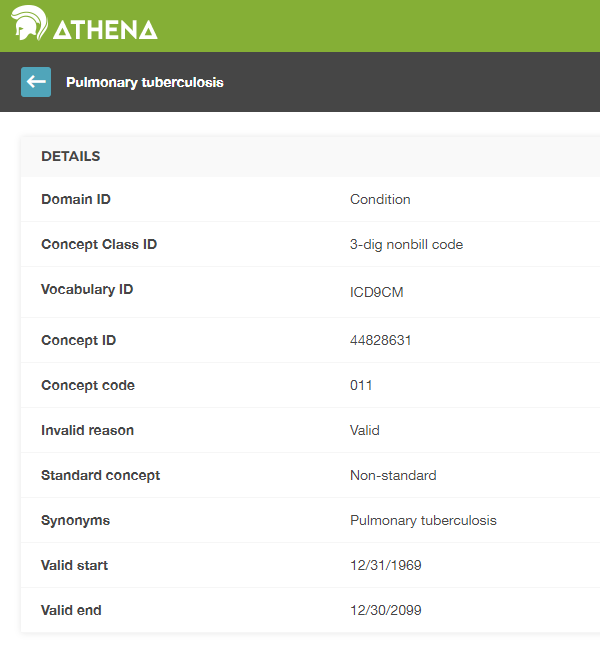
\includegraphics[width=0.75\linewidth]{images/CommonDataModel/pulmTubICD9} 

}

\caption{ICD9CM code for Pulmonary Tuberculosis}\label{fig:pulmTubICD9}
\end{figure}

Without the use of a standard way to represent TB the code 011 could be
interpreted as `Hospital Inpatient (Including Medicare Part A)' in the
UB04 vocabulary, or as `Nervous System Neoplasms without Complications,
Comorbidities' in the DRG vocabulary. This is where Concept IDs, both
Source and Standard, are valuable. The Concept ID that represents the
011 ICD9CM code is
\href{http://athena.ohdsi.org/search-terms/terms/44828631}{44828631}.
This differentiates the ICD9CM from the UBO4 and from the DRG. The
Standard Concept that ICD9CM code maps to is
\href{http://athena.ohdsi.org/search-terms/terms/253954}{253954} as
shown in figure \ref{fig:pulmTubMap} by the relationship `Non-standard
to Standard map (OMOP)'. This same mapping relationship exists between
Read, ICD10, CIEL, and MeSH codes, among others, so that any research
that references the standard SNOMED concept is sure to include all
supported source codes.

\begin{figure}
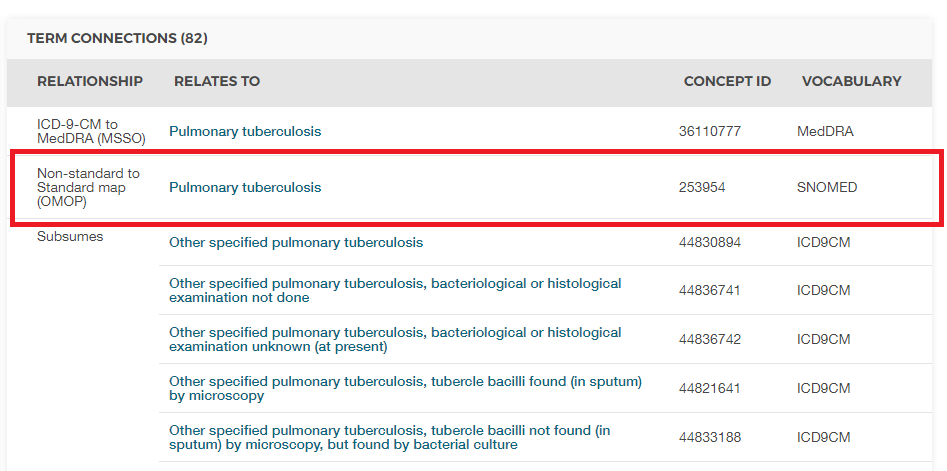
\includegraphics[width=1\linewidth]{images/CommonDataModel/pulmTubMap} \caption{SNOMED code for Pulmonary Tuberculosis}\label{fig:pulmTubMap}
\end{figure}

An example of how this relationship is depicted in the tables is shown
in Table \ref{tab:conditionOccurrence}.

\section{OMOP CDM Standardized
Tables}\label{omop-cdm-standardized-tables}

The OMOP CDM contains 16 Clinical data tables, 10 Vocabulary tables, 2
Metadata tables, 4 Health System data tables, 2 Health Economics data
tables, 3 standardized derived elements, and 2 results schema tables.
These tables are fully specified in the CDM Wiki:
\url{https://github.com/OHDSI/CommonDataModel/wiki}.

To illustrate how these tables are used in practice the data of one
person will be used as a common thread throughout the rest of the
chapter. While part of the CDM the Vocabulary tables are not covered
here, rather, they are detailed in depth in Chapter
\ref{StandardizedVocabularies}.

\subsection{Running Example:
Endometriosis}\label{running-example-endometriosis}

Endometriosis is a painful condition whereby cells normally found in the
lining of a woman's uterus occur elsewhere in the body. Severe cases can
lead to infertility, bowel, and bladder problems. The following sections
will detail one patient's experience with this disease and how her
clinical experience might be represented in the Common Data Model.

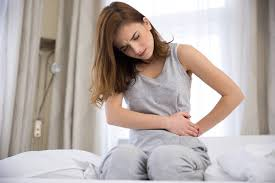
\includegraphics[width=0.5\linewidth]{images/CommonDataModel/Lauren}

Lauren had been experiencing endometriosis symptoms for many year;
however, it took a ruptured cyst in her ovary before she was diagnosed.
You can read more about Lauren at
\url{https://www.endometriosis-uk.org/laurens-story}.

\begin{quote}
Every step of this painfull journey I had to convince everyone how much
pain I was in.
\end{quote}

\subsection{PERSON table}\label{person}

As the Common Data Model is a person-centric model (see section
\ref{model-conv}) let's start with how she would be represented in the
PERSON table.

\textbf{What do we know about Lauren?}

\begin{itemize}
\tightlist
\item
  She is a 36-year-old woman
\item
  Her birthday is 12-March-1982
\item
  She is white
\item
  She is english
\end{itemize}

With that in mind, her PERSON table might look something like this:

\begin{longtable}[]{@{}lll@{}}
\caption{\label{tab:person} The PERSON table.}\tabularnewline
\toprule
\begin{minipage}[b]{0.33\columnwidth}\raggedright\strut
Column Name\strut
\end{minipage} & \begin{minipage}[b]{0.16\columnwidth}\raggedright\strut
Value\strut
\end{minipage} & \begin{minipage}[b]{0.42\columnwidth}\raggedright\strut
Explanation\strut
\end{minipage}\tabularnewline
\midrule
\endfirsthead
\toprule
\begin{minipage}[b]{0.33\columnwidth}\raggedright\strut
Column Name\strut
\end{minipage} & \begin{minipage}[b]{0.16\columnwidth}\raggedright\strut
Value\strut
\end{minipage} & \begin{minipage}[b]{0.42\columnwidth}\raggedright\strut
Explanation\strut
\end{minipage}\tabularnewline
\midrule
\endhead
\begin{minipage}[t]{0.33\columnwidth}\raggedright\strut
PERSON\_ID\strut
\end{minipage} & \begin{minipage}[t]{0.16\columnwidth}\raggedright\strut
1\strut
\end{minipage} & \begin{minipage}[t]{0.42\columnwidth}\raggedright\strut
PERSON\_ID should be an integer, either directly from the source or
generated as part of the build process.\strut
\end{minipage}\tabularnewline
\begin{minipage}[t]{0.33\columnwidth}\raggedright\strut
GENDER\_CONCEPT\_ID\strut
\end{minipage} & \begin{minipage}[t]{0.16\columnwidth}\raggedright\strut
8532\strut
\end{minipage} & \begin{minipage}[t]{0.42\columnwidth}\raggedright\strut
The concept ID referring to female gender is
\href{http://athena.ohdsi.org/search-terms/terms/8532}{8532}.\strut
\end{minipage}\tabularnewline
\begin{minipage}[t]{0.33\columnwidth}\raggedright\strut
YEAR\_OF\_BIRTH\strut
\end{minipage} & \begin{minipage}[t]{0.16\columnwidth}\raggedright\strut
1982\strut
\end{minipage} & \begin{minipage}[t]{0.42\columnwidth}\raggedright\strut
\strut
\end{minipage}\tabularnewline
\begin{minipage}[t]{0.33\columnwidth}\raggedright\strut
MONTH\_OF\_BIRTH\strut
\end{minipage} & \begin{minipage}[t]{0.16\columnwidth}\raggedright\strut
3\strut
\end{minipage} & \begin{minipage}[t]{0.42\columnwidth}\raggedright\strut
\strut
\end{minipage}\tabularnewline
\begin{minipage}[t]{0.33\columnwidth}\raggedright\strut
DAY\_OF\_BIRTH\strut
\end{minipage} & \begin{minipage}[t]{0.16\columnwidth}\raggedright\strut
12\strut
\end{minipage} & \begin{minipage}[t]{0.42\columnwidth}\raggedright\strut
\strut
\end{minipage}\tabularnewline
\begin{minipage}[t]{0.33\columnwidth}\raggedright\strut
BIRTH\_DATETIME\strut
\end{minipage} & \begin{minipage}[t]{0.16\columnwidth}\raggedright\strut
1982-03-12 00:00:00\strut
\end{minipage} & \begin{minipage}[t]{0.42\columnwidth}\raggedright\strut
When the time is not known midnight is used.\strut
\end{minipage}\tabularnewline
\begin{minipage}[t]{0.33\columnwidth}\raggedright\strut
DEATH\_DATETIME\strut
\end{minipage} & \begin{minipage}[t]{0.16\columnwidth}\raggedright\strut
\strut
\end{minipage} & \begin{minipage}[t]{0.42\columnwidth}\raggedright\strut
\strut
\end{minipage}\tabularnewline
\begin{minipage}[t]{0.33\columnwidth}\raggedright\strut
RACE\_CONCEPT\_ID\strut
\end{minipage} & \begin{minipage}[t]{0.16\columnwidth}\raggedright\strut
8527\strut
\end{minipage} & \begin{minipage}[t]{0.42\columnwidth}\raggedright\strut
The concept ID referring to white race is
\href{http://athena.ohdsi.org/search-terms/terms/8527}{8527}.\strut
\end{minipage}\tabularnewline
\begin{minipage}[t]{0.33\columnwidth}\raggedright\strut
ETHNICITY\_CONCEPT\_ID\strut
\end{minipage} & \begin{minipage}[t]{0.16\columnwidth}\raggedright\strut
38003564\strut
\end{minipage} & \begin{minipage}[t]{0.42\columnwidth}\raggedright\strut
Typically hispanic status is stored for ethnicity. The concept ID
\href{http://athena.ohdsi.org/search-terms/terms/38003564}{38003564}
refers to `Not hispanic'.\strut
\end{minipage}\tabularnewline
\begin{minipage}[t]{0.33\columnwidth}\raggedright\strut
LOCATION\_ID\strut
\end{minipage} & \begin{minipage}[t]{0.16\columnwidth}\raggedright\strut
\strut
\end{minipage} & \begin{minipage}[t]{0.42\columnwidth}\raggedright\strut
Her address is not known.\strut
\end{minipage}\tabularnewline
\begin{minipage}[t]{0.33\columnwidth}\raggedright\strut
PROVIDER\_ID\strut
\end{minipage} & \begin{minipage}[t]{0.16\columnwidth}\raggedright\strut
\strut
\end{minipage} & \begin{minipage}[t]{0.42\columnwidth}\raggedright\strut
Her primary care provider is not known.\strut
\end{minipage}\tabularnewline
\begin{minipage}[t]{0.33\columnwidth}\raggedright\strut
CARE\_SITE\_ID\strut
\end{minipage} & \begin{minipage}[t]{0.16\columnwidth}\raggedright\strut
\strut
\end{minipage} & \begin{minipage}[t]{0.42\columnwidth}\raggedright\strut
Her primary care site is not known.\strut
\end{minipage}\tabularnewline
\begin{minipage}[t]{0.33\columnwidth}\raggedright\strut
PERSON\_SOURCE\_VALUE\strut
\end{minipage} & \begin{minipage}[t]{0.16\columnwidth}\raggedright\strut
1\strut
\end{minipage} & \begin{minipage}[t]{0.42\columnwidth}\raggedright\strut
Typically this would be her identifier in the source data, though often
is it the same as the PERSON\_ID.\strut
\end{minipage}\tabularnewline
\begin{minipage}[t]{0.33\columnwidth}\raggedright\strut
GENDER\_SOURCE\_VALUE\strut
\end{minipage} & \begin{minipage}[t]{0.16\columnwidth}\raggedright\strut
F\strut
\end{minipage} & \begin{minipage}[t]{0.42\columnwidth}\raggedright\strut
The gender value as it appears in the source is stored here.\strut
\end{minipage}\tabularnewline
\begin{minipage}[t]{0.33\columnwidth}\raggedright\strut
GENDER\_SOURCE\_ CONCEPT\_ID\strut
\end{minipage} & \begin{minipage}[t]{0.16\columnwidth}\raggedright\strut
0\strut
\end{minipage} & \begin{minipage}[t]{0.42\columnwidth}\raggedright\strut
If the gender value in the source was coded using a vocabulary
recognized by OHDSI, that concept ID would go here. For example, if her
gender was `Sex-F' in the source and it was stated to be in the PCORNet
vocabulary concept ID
\href{http://athena.ohdsi.org/search-terms/terms/44814665}{44814665}
would go in this field.\strut
\end{minipage}\tabularnewline
\begin{minipage}[t]{0.33\columnwidth}\raggedright\strut
RACE\_SOURCE\_VALUE\strut
\end{minipage} & \begin{minipage}[t]{0.16\columnwidth}\raggedright\strut
white\strut
\end{minipage} & \begin{minipage}[t]{0.42\columnwidth}\raggedright\strut
The race value as it appears in the source is stored here.\strut
\end{minipage}\tabularnewline
\begin{minipage}[t]{0.33\columnwidth}\raggedright\strut
RACE\_SOURCE\_CONCEPT\_ID\strut
\end{minipage} & \begin{minipage}[t]{0.16\columnwidth}\raggedright\strut
0\strut
\end{minipage} & \begin{minipage}[t]{0.42\columnwidth}\raggedright\strut
Same principle as GENDER\_SOURCE\_CONCEPT\_ID.\strut
\end{minipage}\tabularnewline
\begin{minipage}[t]{0.33\columnwidth}\raggedright\strut
ETHNICITY\_SOURCE\_VALUE\strut
\end{minipage} & \begin{minipage}[t]{0.16\columnwidth}\raggedright\strut
english\strut
\end{minipage} & \begin{minipage}[t]{0.42\columnwidth}\raggedright\strut
The ethnicity value as it appears in the source is stored here.\strut
\end{minipage}\tabularnewline
\begin{minipage}[t]{0.33\columnwidth}\raggedright\strut
ETHNICITY\_SOURCE\_ CONCEPT\_ID\strut
\end{minipage} & \begin{minipage}[t]{0.16\columnwidth}\raggedright\strut
0\strut
\end{minipage} & \begin{minipage}[t]{0.42\columnwidth}\raggedright\strut
Same principle as GENDER\_SOURCE\_CONCEPT\_ID.\strut
\end{minipage}\tabularnewline
\bottomrule
\end{longtable}

\subsection{OBSERVATION\_PERIOD table}\label{observationPeriod}

The OBSERVATION\_PERIOD table is designed to define the amount of time
for which a patient's clinical events are recorded in the source system.
For US healthcare insurance claims this is typically the enrollment
period of the patient. When working with data from electronic health
records (EHR) often the first record in the system is considered the
OBSERVATION\_PERIOD\_START\_DATE and the latest record is considered the
OBSERVATION\_PERIOD\_END\_DATE with the understanding that only the
clinical events that happened within that particular system were
recorded.

\textbf{How can we determine Lauren's observation period?}

Lauren's information is most similar to EHR data in that we only have
records of her encounters from which to determine her observation
period.

\begin{longtable}[]{@{}llll@{}}
\toprule
Encounter\_ID & Start\_Date & Stop\_Date & EncounterClass\tabularnewline
\midrule
\endhead
70 & 2010-01-06 & 2010-01-06 & outpatient\tabularnewline
80 & 2011-01-06 & 2011-01-06 & outpatient\tabularnewline
90 & 2012-01-06 & 2012-01-06 & outpatient\tabularnewline
100 & 2013-01-07 & 2013-01-07 & outpatient\tabularnewline
101 & 2013-01-14 & 2013-01-14 & ambulatory\tabularnewline
102 & 2013-01-17 & 2013-01-24 & inpatient\tabularnewline
\bottomrule
\end{longtable}

Based on the encounter records her OBSERVATION\_PERIOD table might look
something like this:

\begin{longtable}[]{@{}lll@{}}
\caption{\label{tab:observationPeriod} The OBSERVATION\_PERIOD
table.}\tabularnewline
\toprule
\begin{minipage}[b]{0.33\columnwidth}\raggedright\strut
Column Name\strut
\end{minipage} & \begin{minipage}[b]{0.16\columnwidth}\raggedright\strut
Value\strut
\end{minipage} & \begin{minipage}[b]{0.42\columnwidth}\raggedright\strut
Explanation\strut
\end{minipage}\tabularnewline
\midrule
\endfirsthead
\toprule
\begin{minipage}[b]{0.33\columnwidth}\raggedright\strut
Column Name\strut
\end{minipage} & \begin{minipage}[b]{0.16\columnwidth}\raggedright\strut
Value\strut
\end{minipage} & \begin{minipage}[b]{0.42\columnwidth}\raggedright\strut
Explanation\strut
\end{minipage}\tabularnewline
\midrule
\endhead
\begin{minipage}[t]{0.33\columnwidth}\raggedright\strut
OBSERVATION\_PERIOD\_ID\strut
\end{minipage} & \begin{minipage}[t]{0.16\columnwidth}\raggedright\strut
1\strut
\end{minipage} & \begin{minipage}[t]{0.42\columnwidth}\raggedright\strut
This is typically an autogenerated field that creates a unique id number
for each record in the table.\strut
\end{minipage}\tabularnewline
\begin{minipage}[t]{0.33\columnwidth}\raggedright\strut
PERSON\_ID\strut
\end{minipage} & \begin{minipage}[t]{0.16\columnwidth}\raggedright\strut
1\strut
\end{minipage} & \begin{minipage}[t]{0.42\columnwidth}\raggedright\strut
This comes from the PERSON table and links PERSON and
OBSERVATION\_PERIOD.\strut
\end{minipage}\tabularnewline
\begin{minipage}[t]{0.33\columnwidth}\raggedright\strut
OBSERVATION\_PERIOD\_ START\_DATE\strut
\end{minipage} & \begin{minipage}[t]{0.16\columnwidth}\raggedright\strut
2010-01-06\strut
\end{minipage} & \begin{minipage}[t]{0.42\columnwidth}\raggedright\strut
This is the start date of her earliest encounter on record.\strut
\end{minipage}\tabularnewline
\begin{minipage}[t]{0.33\columnwidth}\raggedright\strut
OBSERVATION\_PERIOD\_ END\_DATE\strut
\end{minipage} & \begin{minipage}[t]{0.16\columnwidth}\raggedright\strut
2013-01-24\strut
\end{minipage} & \begin{minipage}[t]{0.42\columnwidth}\raggedright\strut
This is the end date of her latest encounter on record.\strut
\end{minipage}\tabularnewline
\begin{minipage}[t]{0.33\columnwidth}\raggedright\strut
PERIOD\_TYPE\_CONCEPT\_ID\strut
\end{minipage} & \begin{minipage}[t]{0.16\columnwidth}\raggedright\strut
44814725\strut
\end{minipage} & \begin{minipage}[t]{0.42\columnwidth}\raggedright\strut
The best option in the Vocabulary with the concept class `Obs Period
Type' is
\href{http://athena.ohdsi.org/search-terms/terms/44814724}{44814724},
which stands for `Period covering healthcare encounters'.\strut
\end{minipage}\tabularnewline
\bottomrule
\end{longtable}

\subsection{VISIT\_OCCURRENCE}\label{visitOccurrence}

The VISIT\_OCCURRENCE table houses information about a patient's
encounters with the health care system. Within the OHDSI vernacular
these are referred to as visits and are considered to be discreet
events. There are 12 categories of visits though the most common are
inpatient, outpatient, emergency and long term care.

\textbf{How do we represent Lauren's encounters as visits?}

Revisting the encounters we used to determine her observation period:

\begin{longtable}[]{@{}llll@{}}
\toprule
Encounter\_ID & Start\_Date & Stop\_Date & EncounterClass\tabularnewline
\midrule
\endhead
70 & 2010-01-06 & 2010-01-06 & outpatient\tabularnewline
80 & 2011-01-06 & 2011-01-06 & outpatient\tabularnewline
90 & 2012-01-06 & 2012-01-06 & outpatient\tabularnewline
100 & 2013-01-07 & 2013-01-07 & outpatient\tabularnewline
101 & 2013-01-14 & 2013-01-14 & ambulatory\tabularnewline
\textbf{102} & \textbf{2013-01-17} & \textbf{2013-01-24} &
\textbf{inpatient}\tabularnewline
\bottomrule
\end{longtable}

As an example let's represent the inpatient encounter as a record in the
VISIT\_OCCURRENCE table.

\begin{longtable}[]{@{}lll@{}}
\caption{\label{tab:visitOccurrence} The VISIT\_OCCURRENCE
table.}\tabularnewline
\toprule
\begin{minipage}[b]{0.25\columnwidth}\raggedright\strut
Column Name\strut
\end{minipage} & \begin{minipage}[b]{0.17\columnwidth}\raggedright\strut
Value\strut
\end{minipage} & \begin{minipage}[b]{0.49\columnwidth}\raggedright\strut
Explanation\strut
\end{minipage}\tabularnewline
\midrule
\endfirsthead
\toprule
\begin{minipage}[b]{0.25\columnwidth}\raggedright\strut
Column Name\strut
\end{minipage} & \begin{minipage}[b]{0.17\columnwidth}\raggedright\strut
Value\strut
\end{minipage} & \begin{minipage}[b]{0.49\columnwidth}\raggedright\strut
Explanation\strut
\end{minipage}\tabularnewline
\midrule
\endhead
\begin{minipage}[t]{0.25\columnwidth}\raggedright\strut
VISIT\_OCCURRENCE\_ID\strut
\end{minipage} & \begin{minipage}[t]{0.17\columnwidth}\raggedright\strut
514\strut
\end{minipage} & \begin{minipage}[t]{0.49\columnwidth}\raggedright\strut
This is typically an autogenerated field that creates a unique id number
for each visit on the person's record in the converted CDM
database.\strut
\end{minipage}\tabularnewline
\begin{minipage}[t]{0.25\columnwidth}\raggedright\strut
PERSON\_ID\strut
\end{minipage} & \begin{minipage}[t]{0.17\columnwidth}\raggedright\strut
1\strut
\end{minipage} & \begin{minipage}[t]{0.49\columnwidth}\raggedright\strut
This comes from the PERSON table and links PERSON and
VISIT\_OCCURRENCE.\strut
\end{minipage}\tabularnewline
\begin{minipage}[t]{0.25\columnwidth}\raggedright\strut
VISIT\_CONCEPT\_ID\strut
\end{minipage} & \begin{minipage}[t]{0.17\columnwidth}\raggedright\strut
9201\strut
\end{minipage} & \begin{minipage}[t]{0.49\columnwidth}\raggedright\strut
The concept ID referring to an inpatient visit is
\href{http://athena.ohdsi.org/search-terms/terms/9201}{9201}.\strut
\end{minipage}\tabularnewline
\begin{minipage}[t]{0.25\columnwidth}\raggedright\strut
VISIT\_START\_DATE\strut
\end{minipage} & \begin{minipage}[t]{0.17\columnwidth}\raggedright\strut
2013-01-17\strut
\end{minipage} & \begin{minipage}[t]{0.49\columnwidth}\raggedright\strut
The start date of the visit.\strut
\end{minipage}\tabularnewline
\begin{minipage}[t]{0.25\columnwidth}\raggedright\strut
VISIT\_START\_DATETIME\strut
\end{minipage} & \begin{minipage}[t]{0.17\columnwidth}\raggedright\strut
2013-01-17 00:00:00\strut
\end{minipage} & \begin{minipage}[t]{0.49\columnwidth}\raggedright\strut
The date and time of the visit started. When time is unknown midnight is
used.\strut
\end{minipage}\tabularnewline
\begin{minipage}[t]{0.25\columnwidth}\raggedright\strut
VISIT\_END\_DATE\strut
\end{minipage} & \begin{minipage}[t]{0.17\columnwidth}\raggedright\strut
2013-01-24\strut
\end{minipage} & \begin{minipage}[t]{0.49\columnwidth}\raggedright\strut
The end date of the visit. If this is a one-day visit the end date
should match the start date.\strut
\end{minipage}\tabularnewline
\begin{minipage}[t]{0.25\columnwidth}\raggedright\strut
VISIT\_END\_DATETIME\strut
\end{minipage} & \begin{minipage}[t]{0.17\columnwidth}\raggedright\strut
2013-01-24 00:00:00\strut
\end{minipage} & \begin{minipage}[t]{0.49\columnwidth}\raggedright\strut
The date and time of the visit end. If time is unknown midnight is
used.\strut
\end{minipage}\tabularnewline
\begin{minipage}[t]{0.25\columnwidth}\raggedright\strut
VISIT\_TYPE\_CONCEPT\_ID\strut
\end{minipage} & \begin{minipage}[t]{0.17\columnwidth}\raggedright\strut
32034\strut
\end{minipage} & \begin{minipage}[t]{0.49\columnwidth}\raggedright\strut
This column is intended to provide information about the provenance of
the visit record, i.e.~does it come from an insurance claim, hospital
billing record, EHR record, etc. For this example the concept ID
\href{http://athena.ohdsi.org/search-terms/terms/32035}{32035} is used
as the encounters are similar to electronic health records\strut
\end{minipage}\tabularnewline
\begin{minipage}[t]{0.25\columnwidth}\raggedright\strut
PROVIDER\_ID*\strut
\end{minipage} & \begin{minipage}[t]{0.17\columnwidth}\raggedright\strut
NULL\strut
\end{minipage} & \begin{minipage}[t]{0.49\columnwidth}\raggedright\strut
If the encounter record has a provider associated, the id for that
provider goes in this field. This should be the PROVIDER\_ID from the
PROVIDER table that represents the provider on the encounter.\strut
\end{minipage}\tabularnewline
\begin{minipage}[t]{0.25\columnwidth}\raggedright\strut
CARE\_SITE\_ID\strut
\end{minipage} & \begin{minipage}[t]{0.17\columnwidth}\raggedright\strut
NULL\strut
\end{minipage} & \begin{minipage}[t]{0.49\columnwidth}\raggedright\strut
If the encounter record has a care site associated, the id for that care
site goes in this field. This should be the CARE\_SITE\_ID from the
CARE\_SITE table that codes for the care site on the encounter.\strut
\end{minipage}\tabularnewline
\begin{minipage}[t]{0.25\columnwidth}\raggedright\strut
VISIT\_SOURCE\_VALUE\strut
\end{minipage} & \begin{minipage}[t]{0.17\columnwidth}\raggedright\strut
inpatient\strut
\end{minipage} & \begin{minipage}[t]{0.49\columnwidth}\raggedright\strut
The visit value as it appears in the source goes here. In this context
`visit' means outpatient, inpatient, emergency, etc.\strut
\end{minipage}\tabularnewline
\begin{minipage}[t]{0.25\columnwidth}\raggedright\strut
VISIT\_SOURCE\_ CONCEPT\_ID\strut
\end{minipage} & \begin{minipage}[t]{0.17\columnwidth}\raggedright\strut
0\strut
\end{minipage} & \begin{minipage}[t]{0.49\columnwidth}\raggedright\strut
If the visit value from the source is coded using a vocabulary that is
recognized by OHDSI, the concept ID that represents the visit source
value would go here.\strut
\end{minipage}\tabularnewline
\begin{minipage}[t]{0.25\columnwidth}\raggedright\strut
ADMITTED\_FROM\_ CONCEPT\_ID\strut
\end{minipage} & \begin{minipage}[t]{0.17\columnwidth}\raggedright\strut
0\strut
\end{minipage} & \begin{minipage}[t]{0.49\columnwidth}\raggedright\strut
If known, this is the concept ID that represents where the patient was
admitted from. This concept should have the concept class `Place of
Service' and the domain `Visit'. For example, if a patient was admitted
to the hospital from home, the concept ID would be
\href{http://athena.ohdsi.org/search-terms/terms/8536}{8536}.\strut
\end{minipage}\tabularnewline
\begin{minipage}[t]{0.25\columnwidth}\raggedright\strut
ADMITTED\_FROM\_ SOURCE\_VALUE\strut
\end{minipage} & \begin{minipage}[t]{0.17\columnwidth}\raggedright\strut
NULL\strut
\end{minipage} & \begin{minipage}[t]{0.49\columnwidth}\raggedright\strut
This is the value from the source that represents where the patient was
admitted from. Using the above example, this would be `home'.\strut
\end{minipage}\tabularnewline
\begin{minipage}[t]{0.25\columnwidth}\raggedright\strut
DISCHARGE\_TO\_ CONCEPT\_ID\strut
\end{minipage} & \begin{minipage}[t]{0.17\columnwidth}\raggedright\strut
0\strut
\end{minipage} & \begin{minipage}[t]{0.49\columnwidth}\raggedright\strut
If known, this is the concept ID that represents where the patient was
discharged to. This concept should have the concept class `Place of
Service' and the domain `Visit'. For example, if a patient was released
to an assisted living facility, the concept ID would be
\href{http://athena.ohdsi.org/search-terms/terms/8615}{8615}.\strut
\end{minipage}\tabularnewline
\begin{minipage}[t]{0.25\columnwidth}\raggedright\strut
DISCHARGE\_TO\_ SOURCE\_VALUE\strut
\end{minipage} & \begin{minipage}[t]{0.17\columnwidth}\raggedright\strut
0\strut
\end{minipage} & \begin{minipage}[t]{0.49\columnwidth}\raggedright\strut
This is the value from the source that represents where the patient was
discharged to. Using the above example, this would be `assisted living
facility'.\strut
\end{minipage}\tabularnewline
\begin{minipage}[t]{0.25\columnwidth}\raggedright\strut
PRECEDING\_VISIT\_ OCCURRENCE\_ID\strut
\end{minipage} & \begin{minipage}[t]{0.17\columnwidth}\raggedright\strut
NULL\strut
\end{minipage} & \begin{minipage}[t]{0.49\columnwidth}\raggedright\strut
The VISIT\_OCCURRENCE\_ID for the visit immediately preceding the
current one in time for the patient.\strut
\end{minipage}\tabularnewline
\bottomrule
\end{longtable}

*A patient may interact with multiple health care providers during one
visit, as is often the case with inpatient stays. These interactions can
be recorded in the VISIT\_DETAIL table. While not covered in depth in
this chapter, you can read more about the VISIT\_DETAIL table on the
\href{https://github.com/OHDSI/CommonDataModel/wiki/VISIT_DETAIL}{CDM
wiki}.

\subsection{CONDITION\_OCCURRENCE}\label{conditionOccurrence}

Records in the CONDITION\_OCCURRENCE table are diagnoses, signs, or
symptoms of a condition either observed by a Provider or reported by the
patient.

\textbf{What are Lauren's conditions?}

Revisiting her account she says:

\begin{quote}
About 3 years ago I noticed my periods, which had also been painful,
were getting increasingly more painful. I started becoming aware of a
sharp jabbing pain right by my colon and feeling tender and bloated
around my tailbone and lower pelvis area. My periods had become so
painful that I was missing 1-2 days of work a month. Painkillers
sometimes dulled the pain, but usually they didn't do much.
\end{quote}

The SNOMED code for painful menstruation cramps, otherwise known as
dysmenorrhea, is 266599000. Table \ref{tab:conditionOccurrence} shows
how that would be represented in the CONDITION\_OCCURRENCE table:

\begin{longtable}[]{@{}lll@{}}
\caption{\label{tab:conditionOccurrence} The CONDITION\_OCCURRENCE
table.}\tabularnewline
\toprule
\begin{minipage}[b]{0.27\columnwidth}\raggedright\strut
Column\strut
\end{minipage} & \begin{minipage}[b]{0.14\columnwidth}\raggedright\strut
Value\strut
\end{minipage} & \begin{minipage}[b]{0.50\columnwidth}\raggedright\strut
Explanation\strut
\end{minipage}\tabularnewline
\midrule
\endfirsthead
\toprule
\begin{minipage}[b]{0.27\columnwidth}\raggedright\strut
Column\strut
\end{minipage} & \begin{minipage}[b]{0.14\columnwidth}\raggedright\strut
Value\strut
\end{minipage} & \begin{minipage}[b]{0.50\columnwidth}\raggedright\strut
Explanation\strut
\end{minipage}\tabularnewline
\midrule
\endhead
\begin{minipage}[t]{0.27\columnwidth}\raggedright\strut
CONDITION\_OCCURRENCE\_ID\strut
\end{minipage} & \begin{minipage}[t]{0.14\columnwidth}\raggedright\strut
964\strut
\end{minipage} & \begin{minipage}[t]{0.50\columnwidth}\raggedright\strut
This is typically an autogenerated field that creates a unique id number
for each condition on the person's record in the converted CDM
database.\strut
\end{minipage}\tabularnewline
\begin{minipage}[t]{0.27\columnwidth}\raggedright\strut
PERSON\_ID\strut
\end{minipage} & \begin{minipage}[t]{0.14\columnwidth}\raggedright\strut
1\strut
\end{minipage} & \begin{minipage}[t]{0.50\columnwidth}\raggedright\strut
This comes from the PERSON table and links PERSON and
CONDITION\_OCCURRENCE.\strut
\end{minipage}\tabularnewline
\begin{minipage}[t]{0.27\columnwidth}\raggedright\strut
CONDITION\_CONCEPT\_ID\strut
\end{minipage} & \begin{minipage}[t]{0.14\columnwidth}\raggedright\strut
194696\strut
\end{minipage} & \begin{minipage}[t]{0.50\columnwidth}\raggedright\strut
The concept ID that represents the SNOMED code 266599000 is
\href{http://athena.ohdsi.org/search-terms/terms/194696}{194696}\strut
\end{minipage}\tabularnewline
\begin{minipage}[t]{0.27\columnwidth}\raggedright\strut
CONDITION\_START\_DATE\strut
\end{minipage} & \begin{minipage}[t]{0.14\columnwidth}\raggedright\strut
2010-01-06\strut
\end{minipage} & \begin{minipage}[t]{0.50\columnwidth}\raggedright\strut
The date when the instance of the Condition is recorded.\strut
\end{minipage}\tabularnewline
\begin{minipage}[t]{0.27\columnwidth}\raggedright\strut
CONDITION\_START\_ DATETIME\strut
\end{minipage} & \begin{minipage}[t]{0.14\columnwidth}\raggedright\strut
2010-01-06 00:00:00\strut
\end{minipage} & \begin{minipage}[t]{0.50\columnwidth}\raggedright\strut
The date and time when the instance of the Condition is recorded.
Midnight is used when the time is unknown\strut
\end{minipage}\tabularnewline
\begin{minipage}[t]{0.27\columnwidth}\raggedright\strut
CONDITION\_END\_DATE\strut
\end{minipage} & \begin{minipage}[t]{0.14\columnwidth}\raggedright\strut
NULL\strut
\end{minipage} & \begin{minipage}[t]{0.50\columnwidth}\raggedright\strut
If known, this is the date when the instance of the Condition is
considered to have ended.\strut
\end{minipage}\tabularnewline
\begin{minipage}[t]{0.27\columnwidth}\raggedright\strut
CONDITION\_END\_ DATETIME\strut
\end{minipage} & \begin{minipage}[t]{0.14\columnwidth}\raggedright\strut
NULL\strut
\end{minipage} & \begin{minipage}[t]{0.50\columnwidth}\raggedright\strut
If known, this is the date and time when the instance of the Condition
is considered to have ended.\strut
\end{minipage}\tabularnewline
\begin{minipage}[t]{0.27\columnwidth}\raggedright\strut
CONDITION\_TYPE\_ CONCEPT\_ID\strut
\end{minipage} & \begin{minipage}[t]{0.14\columnwidth}\raggedright\strut
32020\strut
\end{minipage} & \begin{minipage}[t]{0.50\columnwidth}\raggedright\strut
This column is intended to provide information about the provenance of
the condition, i.e.~does it come from an insurance claim, hospital
billing record, EHR record, etc. For this example the concept ID
\href{http://athena.ohdsi.org/search-terms/terms/32020}{32020} is used
as the encounters are similar to electronic health records. Concept IDs
in this field should be in the `Condition Type' vocabulary.\strut
\end{minipage}\tabularnewline
\begin{minipage}[t]{0.27\columnwidth}\raggedright\strut
CONDITION\_STATUS\_ CONCEPT\_ID\strut
\end{minipage} & \begin{minipage}[t]{0.14\columnwidth}\raggedright\strut
0\strut
\end{minipage} & \begin{minipage}[t]{0.50\columnwidth}\raggedright\strut
If known, the CONDITION\_STATUS\_CONCEPT\_ID represents when and/or how
the condition was diagnosed. For example, a condition could be an
admitting diagnosis, in which case the concept ID
\href{http://athena.ohdsi.org/search-terms/terms/4203942}{4203942} would
be used.\strut
\end{minipage}\tabularnewline
\begin{minipage}[t]{0.27\columnwidth}\raggedright\strut
STOP\_REASON\strut
\end{minipage} & \begin{minipage}[t]{0.14\columnwidth}\raggedright\strut
NULL\strut
\end{minipage} & \begin{minipage}[t]{0.50\columnwidth}\raggedright\strut
If known, the reason that the Condition was no longer present, as
indicated in the source data.\strut
\end{minipage}\tabularnewline
\begin{minipage}[t]{0.27\columnwidth}\raggedright\strut
PROVIDER\_ID\strut
\end{minipage} & \begin{minipage}[t]{0.14\columnwidth}\raggedright\strut
NULL\strut
\end{minipage} & \begin{minipage}[t]{0.50\columnwidth}\raggedright\strut
If the condition record has a diagnosing provider listed, the id for
that provider goes in this field. This should be the PROVIDER\_ID from
the PROVIDER table that represents the provider on the encounter.\strut
\end{minipage}\tabularnewline
\begin{minipage}[t]{0.27\columnwidth}\raggedright\strut
VISIT\_OCCURRENCE\_ID\strut
\end{minipage} & \begin{minipage}[t]{0.14\columnwidth}\raggedright\strut
509\strut
\end{minipage} & \begin{minipage}[t]{0.50\columnwidth}\raggedright\strut
If known, this is the visit (represented as VISIT\_OCCURRENCE\_ID taken
from the VISIT\_OCCURRENCE table) during which the condition was
diagnosed.\strut
\end{minipage}\tabularnewline
\begin{minipage}[t]{0.27\columnwidth}\raggedright\strut
VISIT\_DETAIL\_ID\strut
\end{minipage} & \begin{minipage}[t]{0.14\columnwidth}\raggedright\strut
NULL\strut
\end{minipage} & \begin{minipage}[t]{0.50\columnwidth}\raggedright\strut
If known, this is the visit detail encounter (represented as
VISIT\_DETAIL\_ID from the VISIT\_DETAIL table) during which the
condition was diagnosed.\strut
\end{minipage}\tabularnewline
\begin{minipage}[t]{0.27\columnwidth}\raggedright\strut
CONDITION\_SOURCE\_VALUE\strut
\end{minipage} & \begin{minipage}[t]{0.14\columnwidth}\raggedright\strut
266599000\strut
\end{minipage} & \begin{minipage}[t]{0.50\columnwidth}\raggedright\strut
This is the value from the source that represents the condition. In
Lauren's case of dysmenorrhea the SNOMED code for that condition is
stored here and the standard concept ID mapped from that code is stored
in CONDITION\_CONCEPT\_ID.\strut
\end{minipage}\tabularnewline
\begin{minipage}[t]{0.27\columnwidth}\raggedright\strut
CONDITION\_SOURCE\_ CONCEPT\_ID\strut
\end{minipage} & \begin{minipage}[t]{0.14\columnwidth}\raggedright\strut
194696\strut
\end{minipage} & \begin{minipage}[t]{0.50\columnwidth}\raggedright\strut
If the condition value from the source is coded using a vocabulary that
is recognized by OHDSI, the concept ID that represents that value would
go here. In the example of dysmennorhea the source value is a SNOMED
code so the concept ID that represents that code is 194696. In this case
it is the same as the CONDITION\_CONCEPT\_ID since the SNOMED vocabulary
is the standard condition vocabulary\strut
\end{minipage}\tabularnewline
\begin{minipage}[t]{0.27\columnwidth}\raggedright\strut
CONDITION\_STATUS\_ SOURCE\_VALUE\strut
\end{minipage} & \begin{minipage}[t]{0.14\columnwidth}\raggedright\strut
0\strut
\end{minipage} & \begin{minipage}[t]{0.50\columnwidth}\raggedright\strut
If the condition status value from the source is coded using a
vocabulary that is recognized by OHDSI, the concept ID that represents
that source value would go here.\strut
\end{minipage}\tabularnewline
\bottomrule
\end{longtable}

\subsection{DRUG\_EXPOSURE}\label{drugExposure}

The DRUG\_EXPOSURE captures records about the utilization of a Drug when
ingested or otherwise introduced into the body. Drugs include
prescription and over-the-counter medicines, vaccines, and
large-molecule biologic therapies. Radiological devices ingested or
applied locally do not count as Drugs.

Drug Exposure is inferred from clinical events associated with orders,
prescriptions written, pharmacy dispensings, procedural administrations,
and other patient-reported information.

\textbf{What are Lauren's drug exposures?}

We know that Lauren was given 60 acetaminophen 325mg oral tablets for 30
days (NDC code 69842087651) at her visit on 2010-01-06 to help with her
dysmenorrhea pain. Here's how that might look in the DRUG\_EXPOSURE
table:

\begin{longtable}[]{@{}lll@{}}
\caption{\label{tab:drugExposure} The DRUG\_EXPOSURE table.}\tabularnewline
\toprule
\begin{minipage}[b]{0.30\columnwidth}\raggedright\strut
Column\strut
\end{minipage} & \begin{minipage}[b]{0.14\columnwidth}\raggedright\strut
Value\strut
\end{minipage} & \begin{minipage}[b]{0.47\columnwidth}\raggedright\strut
Explanation\strut
\end{minipage}\tabularnewline
\midrule
\endfirsthead
\toprule
\begin{minipage}[b]{0.30\columnwidth}\raggedright\strut
Column\strut
\end{minipage} & \begin{minipage}[b]{0.14\columnwidth}\raggedright\strut
Value\strut
\end{minipage} & \begin{minipage}[b]{0.47\columnwidth}\raggedright\strut
Explanation\strut
\end{minipage}\tabularnewline
\midrule
\endhead
\begin{minipage}[t]{0.30\columnwidth}\raggedright\strut
DRUG\_EXPOSURE\_ID\strut
\end{minipage} & \begin{minipage}[t]{0.14\columnwidth}\raggedright\strut
1001\strut
\end{minipage} & \begin{minipage}[t]{0.47\columnwidth}\raggedright\strut
This is typically an autogenerated field that creates a unique id number
for each drug exposure on the person's record in the converted CDM
database.\strut
\end{minipage}\tabularnewline
\begin{minipage}[t]{0.30\columnwidth}\raggedright\strut
PERSON\_ID\strut
\end{minipage} & \begin{minipage}[t]{0.14\columnwidth}\raggedright\strut
1\strut
\end{minipage} & \begin{minipage}[t]{0.47\columnwidth}\raggedright\strut
This comes from the PERSON table and links PERSON and
DRUG\_EXPOSURE.\strut
\end{minipage}\tabularnewline
\begin{minipage}[t]{0.30\columnwidth}\raggedright\strut
DRUG\_CONCEPT\_ID\strut
\end{minipage} & \begin{minipage}[t]{0.14\columnwidth}\raggedright\strut
1127433\strut
\end{minipage} & \begin{minipage}[t]{0.47\columnwidth}\raggedright\strut
The NDC code for acetaminophen maps to the RxNorm code 313782 which is
represented by the concept ID
\href{http://athena.ohdsi.org/search-terms/terms/1127433}{1127433}.\strut
\end{minipage}\tabularnewline
\begin{minipage}[t]{0.30\columnwidth}\raggedright\strut
DRUG\_EXPOSURE\_ START\_DATE\strut
\end{minipage} & \begin{minipage}[t]{0.14\columnwidth}\raggedright\strut
2010-01-06\strut
\end{minipage} & \begin{minipage}[t]{0.47\columnwidth}\raggedright\strut
The start date of the drug exposure\strut
\end{minipage}\tabularnewline
\begin{minipage}[t]{0.30\columnwidth}\raggedright\strut
DRUG\_EXPOSURE\_ START\_DATETIME\strut
\end{minipage} & \begin{minipage}[t]{0.14\columnwidth}\raggedright\strut
2010-01-06 00:00:00\strut
\end{minipage} & \begin{minipage}[t]{0.47\columnwidth}\raggedright\strut
The start date and time of the drug exposure. Midnight is used when the
time is not known.\strut
\end{minipage}\tabularnewline
\begin{minipage}[t]{0.30\columnwidth}\raggedright\strut
DRUG\_EXPOSURE\_ END\_DATE\strut
\end{minipage} & \begin{minipage}[t]{0.14\columnwidth}\raggedright\strut
2010-02-05\strut
\end{minipage} & \begin{minipage}[t]{0.47\columnwidth}\raggedright\strut
The end date of the drug exposure. Depending on different sources, it
could be a known or an inferred date and denotes the last day at which
the patient was still exposed to the drug. In this case the end is
inferred since we know Lauren had a 30 days supply.\strut
\end{minipage}\tabularnewline
\begin{minipage}[t]{0.30\columnwidth}\raggedright\strut
DRUG\_EXPOSURE\_ END\_DATETIME\strut
\end{minipage} & \begin{minipage}[t]{0.14\columnwidth}\raggedright\strut
2010-02-05 00:00:00\strut
\end{minipage} & \begin{minipage}[t]{0.47\columnwidth}\raggedright\strut
The end date and time of the drug exposure. Similar rules apply as to
DRUG\_EXPOSURE\_END\_DATE. Midnight is used when time is unknown\strut
\end{minipage}\tabularnewline
\begin{minipage}[t]{0.30\columnwidth}\raggedright\strut
VERBATIM\_END\_DATE\strut
\end{minipage} & \begin{minipage}[t]{0.14\columnwidth}\raggedright\strut
NULL\strut
\end{minipage} & \begin{minipage}[t]{0.47\columnwidth}\raggedright\strut
If the source provides an end date rather than just days supply that
date goes here.\strut
\end{minipage}\tabularnewline
\begin{minipage}[t]{0.30\columnwidth}\raggedright\strut
DRUG\_TYPE\_ CONCEPT\_ID\strut
\end{minipage} & \begin{minipage}[t]{0.14\columnwidth}\raggedright\strut
38000177\strut
\end{minipage} & \begin{minipage}[t]{0.47\columnwidth}\raggedright\strut
This column is intended to provide information about the provenance of
the drug, i.e.~does it come from an insurance claim, prescription
record, etc. For this example the concept ID
\href{http://athena.ohdsi.org/search-terms/terms/38000177}{38000177} is
used as the drug record is from a written prescription. Concept IDs in
this field should be in the `Drug Type' vocabulary.\strut
\end{minipage}\tabularnewline
\begin{minipage}[t]{0.30\columnwidth}\raggedright\strut
STOP\_REASON\strut
\end{minipage} & \begin{minipage}[t]{0.14\columnwidth}\raggedright\strut
NULL\strut
\end{minipage} & \begin{minipage}[t]{0.47\columnwidth}\raggedright\strut
The reason the Drug was stopped. Reasons include regimen completed,
changed, removed, etc.\strut
\end{minipage}\tabularnewline
\begin{minipage}[t]{0.30\columnwidth}\raggedright\strut
REFILLS\strut
\end{minipage} & \begin{minipage}[t]{0.14\columnwidth}\raggedright\strut
NULL\strut
\end{minipage} & \begin{minipage}[t]{0.47\columnwidth}\raggedright\strut
The number of refills after the initial prescription. The initial
prescription is not counted, values start with null. In the case of
Lauren's acetaminophen she did not have any refills so the value is
NULL.\strut
\end{minipage}\tabularnewline
\begin{minipage}[t]{0.30\columnwidth}\raggedright\strut
QUANTITY\strut
\end{minipage} & \begin{minipage}[t]{0.14\columnwidth}\raggedright\strut
60\strut
\end{minipage} & \begin{minipage}[t]{0.47\columnwidth}\raggedright\strut
The quantity of drug as recorded in the original prescription or
dispensing record.\strut
\end{minipage}\tabularnewline
\begin{minipage}[t]{0.30\columnwidth}\raggedright\strut
DAYS\_SUPPLY\strut
\end{minipage} & \begin{minipage}[t]{0.14\columnwidth}\raggedright\strut
30\strut
\end{minipage} & \begin{minipage}[t]{0.47\columnwidth}\raggedright\strut
The number of days of supply of the medication as prescribed.\strut
\end{minipage}\tabularnewline
\begin{minipage}[t]{0.30\columnwidth}\raggedright\strut
SIG\strut
\end{minipage} & \begin{minipage}[t]{0.14\columnwidth}\raggedright\strut
NULL\strut
\end{minipage} & \begin{minipage}[t]{0.47\columnwidth}\raggedright\strut
The directions (`signetur') on the Drug prescription as recorded in the
original prescription (and printed on the container) or dispensing
record.\strut
\end{minipage}\tabularnewline
\begin{minipage}[t]{0.30\columnwidth}\raggedright\strut
ROUTE\_CONCEPT\_ID\strut
\end{minipage} & \begin{minipage}[t]{0.14\columnwidth}\raggedright\strut
4132161\strut
\end{minipage} & \begin{minipage}[t]{0.47\columnwidth}\raggedright\strut
This concept is meant to represent the route of the drug the patient was
was exposed to. Lauren took her acetaminophen orally so the concept ID
\href{http://athena.ohdsi.org/search-terms/terms/4132161}{4132161} is
used.\strut
\end{minipage}\tabularnewline
\begin{minipage}[t]{0.30\columnwidth}\raggedright\strut
LOT\_NUMBER\strut
\end{minipage} & \begin{minipage}[t]{0.14\columnwidth}\raggedright\strut
NULL\strut
\end{minipage} & \begin{minipage}[t]{0.47\columnwidth}\raggedright\strut
An identifier assigned to a particular quantity or lot of Drug product
from the manufacturer.\strut
\end{minipage}\tabularnewline
\begin{minipage}[t]{0.30\columnwidth}\raggedright\strut
PROVIDER\_ID\strut
\end{minipage} & \begin{minipage}[t]{0.14\columnwidth}\raggedright\strut
NULL\strut
\end{minipage} & \begin{minipage}[t]{0.47\columnwidth}\raggedright\strut
If the drug record has a prescribing provider listed, the id for that
provider goes in this field. This should be the PROVIDER\_ID from the
PROVIDER table that represents the provider on the encounter.\strut
\end{minipage}\tabularnewline
\begin{minipage}[t]{0.30\columnwidth}\raggedright\strut
VISIT\_OCCURRENCE\_ID\strut
\end{minipage} & \begin{minipage}[t]{0.14\columnwidth}\raggedright\strut
509\strut
\end{minipage} & \begin{minipage}[t]{0.47\columnwidth}\raggedright\strut
If known, this is the visit (represented as VISIT\_OCCURRENCE\_ID taken
from the VISIT\_OCCURRENCE table) during which the drug was
prescribed.\strut
\end{minipage}\tabularnewline
\begin{minipage}[t]{0.30\columnwidth}\raggedright\strut
VISIT\_DETAIL\_ID\strut
\end{minipage} & \begin{minipage}[t]{0.14\columnwidth}\raggedright\strut
NULL\strut
\end{minipage} & \begin{minipage}[t]{0.47\columnwidth}\raggedright\strut
If known, this is the visit detail (represented as VISIT\_DETAIL\_ID
taken from the VISIT\_DETAIL table) during which the drug was
prescribed.\strut
\end{minipage}\tabularnewline
\begin{minipage}[t]{0.30\columnwidth}\raggedright\strut
DRUG\_SOURCE\_VALUE\strut
\end{minipage} & \begin{minipage}[t]{0.14\columnwidth}\raggedright\strut
69842087651\strut
\end{minipage} & \begin{minipage}[t]{0.47\columnwidth}\raggedright\strut
This is the source code for the Drug as it appears in the source data.
In Lauren's case she was prescribed acetaminophen and the NDC code is
stored here.\strut
\end{minipage}\tabularnewline
\begin{minipage}[t]{0.30\columnwidth}\raggedright\strut
DRUG\_SOURCE\_ CONCEPT\_ID\strut
\end{minipage} & \begin{minipage}[t]{0.14\columnwidth}\raggedright\strut
750264\strut
\end{minipage} & \begin{minipage}[t]{0.47\columnwidth}\raggedright\strut
This is the concept ID that represents the drug source value. In this
example the concept ID is
\href{http://athena.ohdsi.org/search-terms/terms/750264}{750264}.\strut
\end{minipage}\tabularnewline
\begin{minipage}[t]{0.30\columnwidth}\raggedright\strut
ROUTE\_SOURCE\_VALUE\strut
\end{minipage} & \begin{minipage}[t]{0.14\columnwidth}\raggedright\strut
NULL\strut
\end{minipage} & \begin{minipage}[t]{0.47\columnwidth}\raggedright\strut
The information about the route of administration as detailed in the
source.\strut
\end{minipage}\tabularnewline
\begin{minipage}[t]{0.30\columnwidth}\raggedright\strut
DOSE\_UNIT\_ SOURCE\_VALUE\strut
\end{minipage} & \begin{minipage}[t]{0.14\columnwidth}\raggedright\strut
NULL\strut
\end{minipage} & \begin{minipage}[t]{0.47\columnwidth}\raggedright\strut
The information about the dose unit as detailed in the source.\strut
\end{minipage}\tabularnewline
\bottomrule
\end{longtable}

\subsection{PROCEDURE\_OCCURRENCE}\label{procedureOccurrence}

The PROCEDURE\_OCCURRENCE table contains records of activities or
processes ordered by, or carried out by, a healthcare provider on the
patient to have a diagnostic or therapeutic purpose. Procedures are
present in various data sources in different forms with varying levels
of standardization. For example:

\begin{itemize}
\tightlist
\item
  Medical Claims include procedure codes that are submitted as part of a
  claim for health services rendered, including procedures performed.
\item
  Electronic Health Records that capture procedures as orders.
\end{itemize}

\textbf{What procedures did Lauren have?} From her description we know
she had a ultrasound of her left ovary on 2013-01-14 that showed a 4x5cm
cyst. Here's how that would look in the PROCEDURE\_OCCURRENCE table:

\begin{longtable}[]{@{}lll@{}}
\caption{\label{tab:procedureOccurrence} The PROCEDURE\_OCCURRENCE
table.}\tabularnewline
\toprule
\begin{minipage}[b]{0.30\columnwidth}\raggedright\strut
Column\strut
\end{minipage} & \begin{minipage}[b]{0.14\columnwidth}\raggedright\strut
Value\strut
\end{minipage} & \begin{minipage}[b]{0.47\columnwidth}\raggedright\strut
Explanation\strut
\end{minipage}\tabularnewline
\midrule
\endfirsthead
\toprule
\begin{minipage}[b]{0.30\columnwidth}\raggedright\strut
Column\strut
\end{minipage} & \begin{minipage}[b]{0.14\columnwidth}\raggedright\strut
Value\strut
\end{minipage} & \begin{minipage}[b]{0.47\columnwidth}\raggedright\strut
Explanation\strut
\end{minipage}\tabularnewline
\midrule
\endhead
\begin{minipage}[t]{0.30\columnwidth}\raggedright\strut
PROCEDURE\_OCCURRENCE\_ID\strut
\end{minipage} & \begin{minipage}[t]{0.14\columnwidth}\raggedright\strut
1277\strut
\end{minipage} & \begin{minipage}[t]{0.47\columnwidth}\raggedright\strut
This is typically an autogenerated field that creates a unique id number
for each procedure occurrence on the person's record in the converted
CDM database.\strut
\end{minipage}\tabularnewline
\begin{minipage}[t]{0.30\columnwidth}\raggedright\strut
PERSON\_ID\strut
\end{minipage} & \begin{minipage}[t]{0.14\columnwidth}\raggedright\strut
1\strut
\end{minipage} & \begin{minipage}[t]{0.47\columnwidth}\raggedright\strut
This comes from the PERSON table and links PERSON and
PROCEDURE\_OCCURRENCE\strut
\end{minipage}\tabularnewline
\begin{minipage}[t]{0.30\columnwidth}\raggedright\strut
PROCEDURE\_CONCEPT\_ID\strut
\end{minipage} & \begin{minipage}[t]{0.14\columnwidth}\raggedright\strut
4127451\strut
\end{minipage} & \begin{minipage}[t]{0.47\columnwidth}\raggedright\strut
The SNOMED procedure code for a pelvic ultrasound is 304435002 which is
represented by the concept ID
\href{http://athena.ohdsi.org/search-terms/terms/4127451}{4127451}.\strut
\end{minipage}\tabularnewline
\begin{minipage}[t]{0.30\columnwidth}\raggedright\strut
PROCEDURE\_DATE\strut
\end{minipage} & \begin{minipage}[t]{0.14\columnwidth}\raggedright\strut
2013-01-14\strut
\end{minipage} & \begin{minipage}[t]{0.47\columnwidth}\raggedright\strut
The date on which the procedure was performed.\strut
\end{minipage}\tabularnewline
\begin{minipage}[t]{0.30\columnwidth}\raggedright\strut
PROCEDURE\_DATETIME\strut
\end{minipage} & \begin{minipage}[t]{0.14\columnwidth}\raggedright\strut
2013-01-14 00:00:00\strut
\end{minipage} & \begin{minipage}[t]{0.47\columnwidth}\raggedright\strut
The date and time on which the procedure was performed. Midnight is used
when time is unknown.\strut
\end{minipage}\tabularnewline
\begin{minipage}[t]{0.30\columnwidth}\raggedright\strut
PROCEDURE\_TYPE\_CONCEPT\_ID\strut
\end{minipage} & \begin{minipage}[t]{0.14\columnwidth}\raggedright\strut
38000275\strut
\end{minipage} & \begin{minipage}[t]{0.47\columnwidth}\raggedright\strut
This column is intended to provide information about the provenance of
the procedure, i.e.~does it come from an insurance claim, EHR order,
etc. For this example the concept ID
\href{http://athena.ohdsi.org/search-terms/terms/38000275}{38000275} is
used as the procedure record is from an EHR record. Concept IDs in this
field should be in the `Procedure Type' vocabulary.\strut
\end{minipage}\tabularnewline
\begin{minipage}[t]{0.30\columnwidth}\raggedright\strut
MODIFIER\_CONCEPT\_ID\strut
\end{minipage} & \begin{minipage}[t]{0.14\columnwidth}\raggedright\strut
0\strut
\end{minipage} & \begin{minipage}[t]{0.47\columnwidth}\raggedright\strut
This is meant for a concept ID representing the modifier on the
procedure. For example, if the record indicated that a CPT4 procedure
was performed bilaterally then the concept ID
\href{http://athena.ohdsi.org/search-terms/terms/42739579}{42739579}
would be used.\strut
\end{minipage}\tabularnewline
\begin{minipage}[t]{0.30\columnwidth}\raggedright\strut
QUANTITY\strut
\end{minipage} & \begin{minipage}[t]{0.14\columnwidth}\raggedright\strut
0\strut
\end{minipage} & \begin{minipage}[t]{0.47\columnwidth}\raggedright\strut
The quantity of procedures ordered or administered.\strut
\end{minipage}\tabularnewline
\begin{minipage}[t]{0.30\columnwidth}\raggedright\strut
PROVIDER\_ID\strut
\end{minipage} & \begin{minipage}[t]{0.14\columnwidth}\raggedright\strut
NULL\strut
\end{minipage} & \begin{minipage}[t]{0.47\columnwidth}\raggedright\strut
If the procedure record has a provider listed, the id for that provider
goes in this field. This should be the PROVIDER\_ID from the PROVIDER
table that represents the provider on the encounter.\strut
\end{minipage}\tabularnewline
\begin{minipage}[t]{0.30\columnwidth}\raggedright\strut
VISIT\_OCCURRENCE\_ID\strut
\end{minipage} & \begin{minipage}[t]{0.14\columnwidth}\raggedright\strut
740\strut
\end{minipage} & \begin{minipage}[t]{0.47\columnwidth}\raggedright\strut
If known, this is the visit (represented as VISIT\_OCCURRENCE\_ID taken
from the VISIT\_OCCURRENCE table) during which the procedure was
performed.\strut
\end{minipage}\tabularnewline
\begin{minipage}[t]{0.30\columnwidth}\raggedright\strut
VISIT\_DETAIL\_ID\strut
\end{minipage} & \begin{minipage}[t]{0.14\columnwidth}\raggedright\strut
NULL\strut
\end{minipage} & \begin{minipage}[t]{0.47\columnwidth}\raggedright\strut
If known, this is the visit detail (represented as VISIT\_DETAIL\_ID
taken from the VISIT\_DETAIL table) during which the procedure was
performed.\strut
\end{minipage}\tabularnewline
\begin{minipage}[t]{0.30\columnwidth}\raggedright\strut
PROCEDURE\_SOURCE\_VALUE\strut
\end{minipage} & \begin{minipage}[t]{0.14\columnwidth}\raggedright\strut
304435002\strut
\end{minipage} & \begin{minipage}[t]{0.47\columnwidth}\raggedright\strut
The source code for the Procedure as it appears in the source data. This
code is mapped to a standard procedure Concept in the Standardized
Vocabularies and the original code is, stored here for reference.\strut
\end{minipage}\tabularnewline
\begin{minipage}[t]{0.30\columnwidth}\raggedright\strut
PROCEDURE\_SOURCE\_ CONCEPT\_ID\strut
\end{minipage} & \begin{minipage}[t]{0.14\columnwidth}\raggedright\strut
4127451\strut
\end{minipage} & \begin{minipage}[t]{0.47\columnwidth}\raggedright\strut
This is the concept ID that represents the procedure source value.\strut
\end{minipage}\tabularnewline
\begin{minipage}[t]{0.30\columnwidth}\raggedright\strut
MODIFIER\_SOURCE\_ VALUE\strut
\end{minipage} & \begin{minipage}[t]{0.14\columnwidth}\raggedright\strut
NULL\strut
\end{minipage} & \begin{minipage}[t]{0.47\columnwidth}\raggedright\strut
The source code for the modifier as it appears in the source data.\strut
\end{minipage}\tabularnewline
\bottomrule
\end{longtable}

\chapter{Standardized Vocabularies}\label{StandardizedVocabularies}

The OMOP Standardized Vocabulary: Christian's (almost) finished paper +
\url{http://www.ohdsi.org/web/wiki/doku.php?id=documentation:vocabulary}

\chapter{Extract Transform Load}\label{ExtractTransformLoad}

Leads: Mui van Zandt \& Clair Blacketer

Business Rules and Conventions: From the CDM Wiki + Themis

Conversion to OMOP CDM (ETL - Extract, Transform, Load):
\url{http://www.ohdsi.org/web/wiki/doku.php?id=documentation:etl_best_practices}

\begin{itemize}
\tightlist
\item
  WhiteRabbit and Rabbit-in-a-Hat:
  \url{http://www.ohdsi.org/web/wiki/doku.php?id=documentation:software:whiterabbit}
\item
  Usagi:
  \url{http://www.ohdsi.org/web/wiki/doku.php?id=documentation:software:usagi}
\item
  Achilles:
  \url{http://www.ohdsi.org/web/wiki/doku.php?id=documentation:software:achilles}
\item
  Athena:
  \url{http://www.ohdsi.org/web/wiki/doku.php?id=documentation:vocabulary_etl}
\end{itemize}

Mapping and QA of codes to Standard Concepts

\begin{itemize}
\tightlist
\item
  Mapping codes locally versus through the OHDSI Standard Vocabularies
\item
  Usagi
\item
  Systematic mapping of Drug codes
\item
  Systematic mapping of Condition codes
\item
  Systematic mapping of Procedure codes
\item
  Systematic mapping of other codes
\end{itemize}

\part{Data Analytics}\label{part-data-analytics}

\chapter{Data Analytics Use Cases}\label{DataAnalyticsUseCases}

\begin{itemize}
\tightlist
\item
  Introduction
\end{itemize}

The OHDSI collaboration focuses on generating reliable evidence from
real-world healthcare data, typically in the form of claims databases or
electronic health record databases. The use cases that OHDSI focuses on
fall into three major buckets and we describe these below. Note, for all
the use cases, the evidence we generate inherits the limitations of the
data; we discuss these limitations at length in Chapters X, Y, and Z.

\begin{itemize}
\tightlist
\item
  Theory
\end{itemize}

\begin{enumerate}
\def\labelenumi{\arabic{enumi}.}
\tightlist
\item
  Population characterization
\end{enumerate}

We can use the data to provide answers to questions about the
charateristics of the patients in each database, the practice of
healthcare, and study how these things change over time.

The data can provide answers to questions like: - for patients newly
diagnosed with atrial fibrillation, how many receive a prescription for
warfarin? - what is the average age of patients who undergo hip
arthoplasty?

\begin{enumerate}
\def\labelenumi{\arabic{enumi}.}
\setcounter{enumi}{1}
\tightlist
\item
  Population-level estimation
\end{enumerate}

To a limited extent, the data can support causal inferences about the
effects of healthcare interventions.

The data can provide answers to questions like: - for patients newly
diagnosed with atrial fibrillation, in the first year after therapy
initiation, does warfarin cause more major bleeds than dabigatran? -
Does the causal effect of metformin on diarrhea vary by age?

\begin{enumerate}
\def\labelenumi{\arabic{enumi}.}
\setcounter{enumi}{2}
\tightlist
\item
  Patient-Level prediction
\end{enumerate}

Based on the collected patient health histories in the database, we can
make patient-level predictions about future health events. - for a
specific patient newly diagnosed with atrial fibrillation, in the first
year after therapy initiation with warfarin, what is the probability the
patient suffers an ischemic stroke?

These tasks overlap to a certain extent. For example, an important
use-case for prediction is to predict an outcome for a specific patient
had drug A been prescribed and also predict the same outcome had drug B
been prescribed. Let's assume that in reality only one of these drugs is
prescribed (say drug A) so we get to see whether the outcome following
treatment with A actually occurs. Since drug B was not prescribed, the
outcome following treatment B, while predictable, is ``counterfactual''
since it is not ever observed. Each of these prediction tasks falls
under patient-level prediction. However, the difference between (or
ratio of) the two outcomes is a unit-level \emph{causal} effect.

There are many important healthcare questions for which OHDSI databases
cannot provide answers. These include:

\begin{itemize}
\tightlist
\item
  Causal effects of interventions compared to placebo. Sometimes it is
  possible to consider the causal effect of a treatment as compared with
  non-treatment but not placebo tretamernt.
\item
  Anything related to over-the-counter medications
\item
  Many outcomes are sparsely recorded if at all. These include
  mortality, behavioral outcomes, lifestyle, and socioeconmic status.
\item
  Since patients tend to encounter the healthcare system when they are
  unwell, measurement of the benefits of treatments can prove elusive.
\end{itemize}

Missingness in OHDSI databases presents subtle challenges. A health
event (e.g., prescription, laboratory value, etc.) that should be
recorded in a database, but isn't, is ``missing.'' The statistics
literature distinguishes between types of missingness such as ``missing
completely at random,'' ``missing at random,'' and ``missing not at
random'' and methods of increasing complexity attempt to address these
types. \citet{perkins2017principled} provide a use introduction to this
topic.

What use cases are often observed? Drug safety, Drug utilization, etc.

\begin{itemize}
\tightlist
\item
  Practice
\end{itemize}

\chapter{OHDSI Analytics Tools}\label{OhdsiAnalyticsTools}

ATLAS:
\url{http://www.ohdsi.org/web/wiki/doku.php?id=documentation:software:atlas}

ARACHNE: Network Research

Methods Library: \url{https://ohdsi.github.io/MethodsLibrary/}

Best practices enforced in all OHDSI methods.

Ethical consideration: e.g.~should always communicate uncertainty.
Prespecification of research questions, etc.

Analytic use cases

What is the difference between characterization, population-level
estimation, patient-level prediction?

Case study: Perhaps on how to install the tools?

\chapter{SQL and R}\label{SqlAndR}

DatabaseConnector and SqlRender

Querying the CDM

Probably borrow heavily from \url{https://github.com/OHDSI/QueryLibrary}

\chapter{Building the building blocks: cohorts}\label{Cohorts}

Introduction: a cohort is a group of people that meet a set of criteria
for a particular span of time etc. Cohorts are used throughout OHDSIs
analytical tools as the primary building blocks.

Using ATLAS: use material from Patrick's tutorial on cohort building

Using SQL: For advanced users, explain how cohorts can be created
programmatically.

Probabilistic cohorts: Aphrodite?

Case study: some example cohort definitions

\chapter{Characterization}\label{Characterization}

ATLAS' incidence rate calculator + cohort characterization tool

FeatureExtraction package:
\url{https://github.com/OHDSI/FeatureExtraction}

Case study: characteristics + IRs of some cohorts

Example .. \url{http://www.pnas.org/content/113/27/7329}

\chapter{Population-level estimation}\label{PopulationLevelEstimation}

\emph{Chapter leads: Martijn Schuemie, David Madigan \& Marc Suchard}

Observational healthcare data, such as administrative claims and
electronic health records, offer opportunities to generate real-world
evidence about the effect of treatments that can meaningfully improve
the lives of patients. In this chapter we focus on population-level
effect estimation, that is, the estimation of average causal effects of
medical interventions on specific health outcomes of interest. In what
follows, we consider two different estimation tasks:

\begin{itemize}
\tightlist
\item
  \textbf{Direct effect estimation}: estimating the effect of an
  exposure on the risk of an outcome, as compared to no exposure.
\item
  \textbf{Comparative effect estimation}: estimation the effect of one
  exposure (the target exposure) on the risk of an outcome, as compared
  to another exposure (the comparator exposure).
\end{itemize}

In both cases, the patient-level causal effect contrasts a factual
outcome, i.e., what happened to the exposed patient, with a
counterfactual outcome, i.e., what would have happened had the exposure
not occurred (direct) or had a different exposure occurred
(comparative). Since any one patient reveals only the factual outcome
(the fundamental problem of causal inference), the various effect
estimation methods employ analytic devices to shed light on the
counterfactual outcomes.

Use-cases for population-level effect estimation include treatment
selection, safety surveillance, and comparative effectiveness. Methods
can test specific hypotheses one-at-a-time (e.g. `signal evaluation') or
explore multiple-hypotheses-at-once (e.g. `signal detection'). In all
cases, the objective remains the same: to produce a high-quality
estimate of the causal effect.

\section{Study designs}\label{study-designs}

Several different study designs can be used to estimate treatment
effects. The main difference between these is how they construct the
(unobserved) counterfactual. Below is a brief discussion of the most
commonly used designs, all of which are implemented as R packages in the
\href{https://ohdsi.github.io/MethodsLibrary/}{OHDSI Methods Library}.

\subsection{Cohort method}\label{cohort-method}

\begin{figure}

{\centering 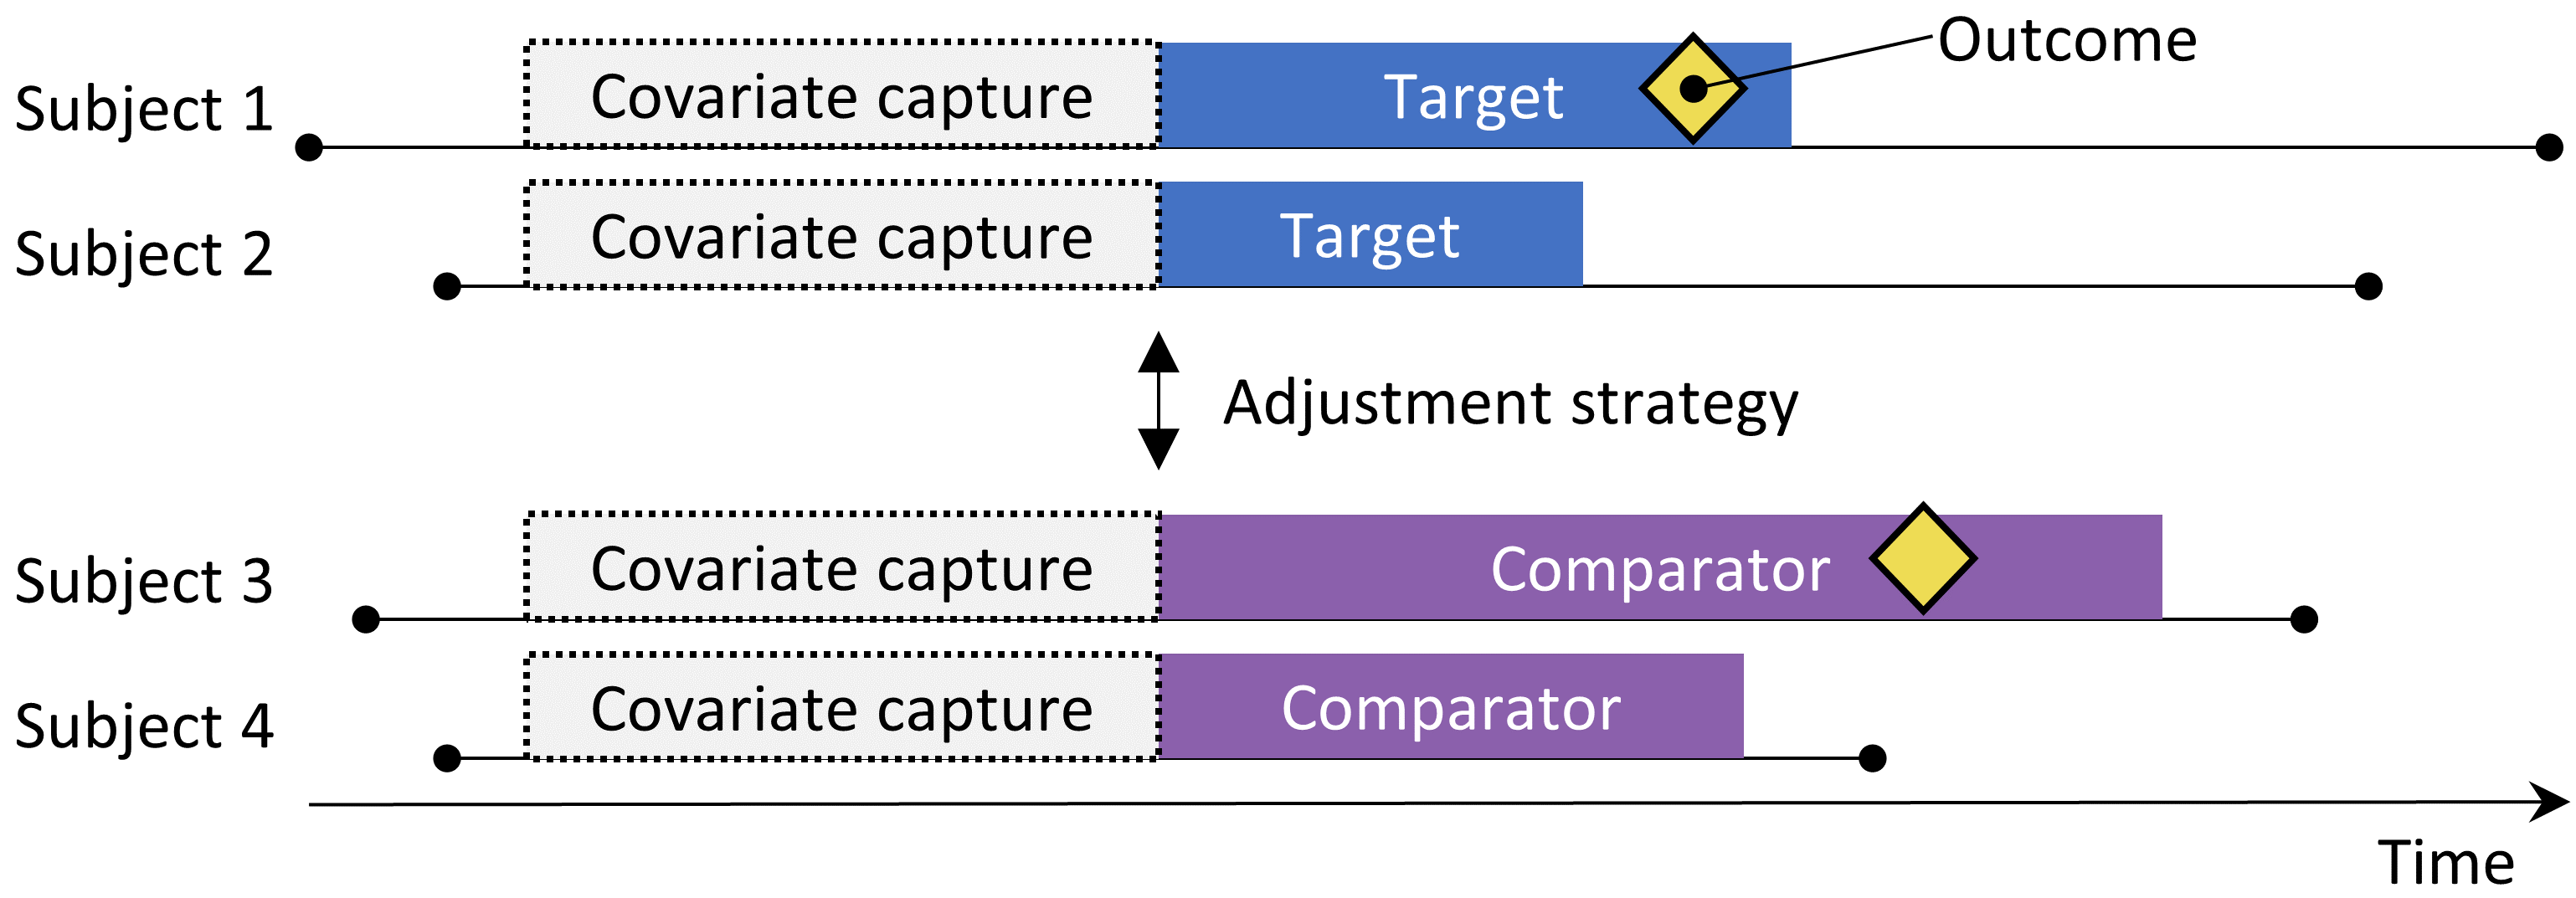
\includegraphics[width=0.9\linewidth]{images/PopulationLevelEstimation/cohortMethod} 

}

\caption{The new-user cohort design. Subjects observed to initiate the target treatment are compared to those initiating the comparator treatment. To adjust for differences between the two treatment groups several adjustment strategies can be used, such as stratification, matching, or weighting by the propensity score, or by adding baseline characateristcs to the outcome model. The chararacteristics included in the propensity model or outcome model are captured prior to treatment initiation.}\label{fig:cohortMethod}
\end{figure}

The new-user cohort method attempts to emulate a randomized clinical
trial \citep{hernan_2016}. Subjects that are observed to initiate one
treatment (the target) are compared to subjects initiating another
treatment (the comparator) and are followed for a specific amount of
time following treatment initiation, for example the time they stay on
the treatment. We can specify the questions we wish to answer in a
cohort study by making the five choices highlighted in Table
\ref{tab:cmChoices}.

\begin{longtable}[]{@{}ll@{}}
\caption{\label{tab:cmChoices} Main design choices in a comparative cohort
design.}\tabularnewline
\toprule
\begin{minipage}[b]{0.23\columnwidth}\raggedright\strut
Choice\strut
\end{minipage} & \begin{minipage}[b]{0.71\columnwidth}\raggedright\strut
Description\strut
\end{minipage}\tabularnewline
\midrule
\endfirsthead
\toprule
\begin{minipage}[b]{0.23\columnwidth}\raggedright\strut
Choice\strut
\end{minipage} & \begin{minipage}[b]{0.71\columnwidth}\raggedright\strut
Description\strut
\end{minipage}\tabularnewline
\midrule
\endhead
\begin{minipage}[t]{0.23\columnwidth}\raggedright\strut
Target cohort\strut
\end{minipage} & \begin{minipage}[t]{0.71\columnwidth}\raggedright\strut
A cohort representing the target treatment\strut
\end{minipage}\tabularnewline
\begin{minipage}[t]{0.23\columnwidth}\raggedright\strut
Comparator cohort\strut
\end{minipage} & \begin{minipage}[t]{0.71\columnwidth}\raggedright\strut
A cohort representing the comparator treatment\strut
\end{minipage}\tabularnewline
\begin{minipage}[t]{0.23\columnwidth}\raggedright\strut
Outcome cohort\strut
\end{minipage} & \begin{minipage}[t]{0.71\columnwidth}\raggedright\strut
A cohort representing the outcome of interest\strut
\end{minipage}\tabularnewline
\begin{minipage}[t]{0.23\columnwidth}\raggedright\strut
Time-at-risk\strut
\end{minipage} & \begin{minipage}[t]{0.71\columnwidth}\raggedright\strut
At what time (often relative to the target and comparator cohort start
and end dates) do we consider the risk of the outcome?\strut
\end{minipage}\tabularnewline
\begin{minipage}[t]{0.23\columnwidth}\raggedright\strut
Model\strut
\end{minipage} & \begin{minipage}[t]{0.71\columnwidth}\raggedright\strut
The model used to estimate the effect while adjusting for differences
between the target and comparator\strut
\end{minipage}\tabularnewline
\bottomrule
\end{longtable}

The choice of model specifies, amongst others, the type of model. For
example, we could use a logistic regression, which evaluates whether or
not the outcome has occurred, and produces an odds ratio. A logistic
regression assumes the time-at-risk is of the same length for both
target and comparator, or irrelevant. Alternatively, we could choose a
Poisson regression which estimates the incidence rate ratio, assuming a
constant incidence rate. Often a Cox regression is used which considers
time to first outcome to estimate the hazard ratio, assuming
proportional hazards.

One crucial difference with a randomized trial is that there is no
randomization, and therefore there might be systematic differences
between the target and comparator populations. Without adjusting for
these differences, estimates are likely to be confounded. A popular
mechanism for adjusting for confounding is the use of Propensity Scores
(PS). The PS is the probability of a subject receiving one treatment
instead of the other, conditional on baseline characteristics.
\citep{rosenbaum_1983} First, a model -- typically a logistic regression
-- is fitted using the observed treatment assignments (target or
comparator), then the model is used to produce the PS for each subject.
In the past, PS were computed based on manually selected
characteristics, and although the CohortMethod package can support such
practices, we prefer the use of large-scale regularized regression using
many generic characteristics. \citep{tian_2018} These characteristics
include demographics, as well as all diagnoses, drug exposures,
measurement, and medical procedures observed prior to treatment
initiation, and exclude the target and comparator treatment. A model
typically involves 10,000 to 100,000 unique characteristics. The PS can
be used in several ways, for example by stratifying the study population
based on the PS, by matching target subjects to comparator subjects with
similar PS, or by weighting subjects using Inverse Probability of
Treatment Weighting (IPTW) derived from the PS. Another strategy for
adjusting for differences between the two groups is to include
additional variables in the outcome model. One major limitation of this
approach is that whereas there often is a wealth of data to fit a
propensity model, with thousands of people in both treatment groups, the
outcomes we study tend to be somewhat rare, causing a paucity of data
when trying to fit elaborate models with the outcome as dependent
variable. One approach is to use both a PS and add the same variables
that were used in the propensity model in the outcome model, thus
adjusting for the same variables twice, but in different ways. The
new-user cohort method inherently is a method for comparative effect
estimation, comparing one treatment to another. It is difficult to use
this method to compare a treatment against no treatment, since it is
hard to define a group of unexposed people that is comparable with the
exposed group. If one wants to use this design for direct effect
estimation, the preferred way is to select a comparator treatment for
the same indication as the exposure of interest, where the comparator
treatment is believed to have no effect on the outcome. Unfortunately,
such a comparator might not always be available.

\subsection{Self-controlled cohort}\label{self-controlled-cohort}

\begin{figure}

{\centering 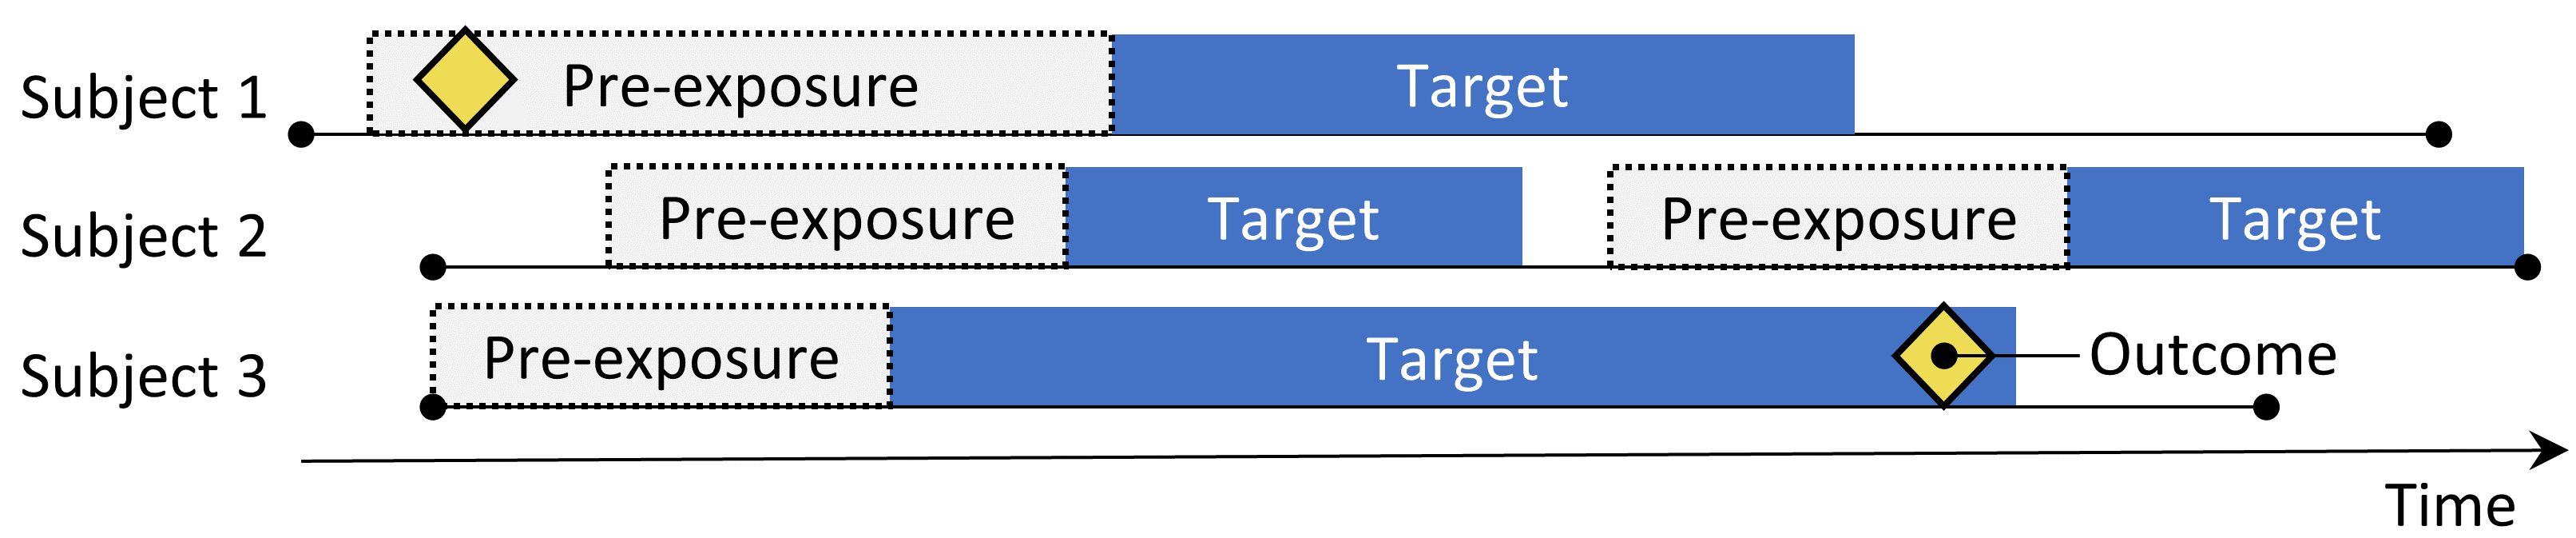
\includegraphics[width=0.9\linewidth]{images/PopulationLevelEstimation/selfControlledCohort} 

}

\caption{The self-controlled cohort design. The rate of outcomes during exposure to the target is compared to the rate of outcomes in the time pre-exposure.}\label{fig:scc}
\end{figure}

The self-controlled cohort (SCC) design \citep{ryan_2013} compares the
rate of outcomes during exposure to the rate of outcomes in the time
just prior to the exposure. The four choices shown in Table
\ref{tab:sccChoices} define a self-controlled cohort question.

\begin{longtable}[]{@{}ll@{}}
\caption{\label{tab:sccChoices} Main design choices in a self-controlled
cohort design.}\tabularnewline
\toprule
\begin{minipage}[b]{0.23\columnwidth}\raggedright\strut
Choice\strut
\end{minipage} & \begin{minipage}[b]{0.71\columnwidth}\raggedright\strut
Description\strut
\end{minipage}\tabularnewline
\midrule
\endfirsthead
\toprule
\begin{minipage}[b]{0.23\columnwidth}\raggedright\strut
Choice\strut
\end{minipage} & \begin{minipage}[b]{0.71\columnwidth}\raggedright\strut
Description\strut
\end{minipage}\tabularnewline
\midrule
\endhead
\begin{minipage}[t]{0.23\columnwidth}\raggedright\strut
Target cohort\strut
\end{minipage} & \begin{minipage}[t]{0.71\columnwidth}\raggedright\strut
A cohort representing the treatment\strut
\end{minipage}\tabularnewline
\begin{minipage}[t]{0.23\columnwidth}\raggedright\strut
Outcome cohort\strut
\end{minipage} & \begin{minipage}[t]{0.71\columnwidth}\raggedright\strut
A cohort representing the outcome of interest\strut
\end{minipage}\tabularnewline
\begin{minipage}[t]{0.23\columnwidth}\raggedright\strut
Time-at-risk\strut
\end{minipage} & \begin{minipage}[t]{0.71\columnwidth}\raggedright\strut
At what time (often relative to the target cohort start and end dates)
do we consider the risk of the outcome?\strut
\end{minipage}\tabularnewline
\begin{minipage}[t]{0.23\columnwidth}\raggedright\strut
Control time\strut
\end{minipage} & \begin{minipage}[t]{0.71\columnwidth}\raggedright\strut
The time period used as the control time\strut
\end{minipage}\tabularnewline
\bottomrule
\end{longtable}

Because the same subject that make up the exposed group are also used as
the control group, no adjustment for between-person differences need to
be made. However, the method is vulnerable to other differences, such as
differences between different time periods.

\subsection{Case-control}\label{case-control}

\begin{figure}

{\centering 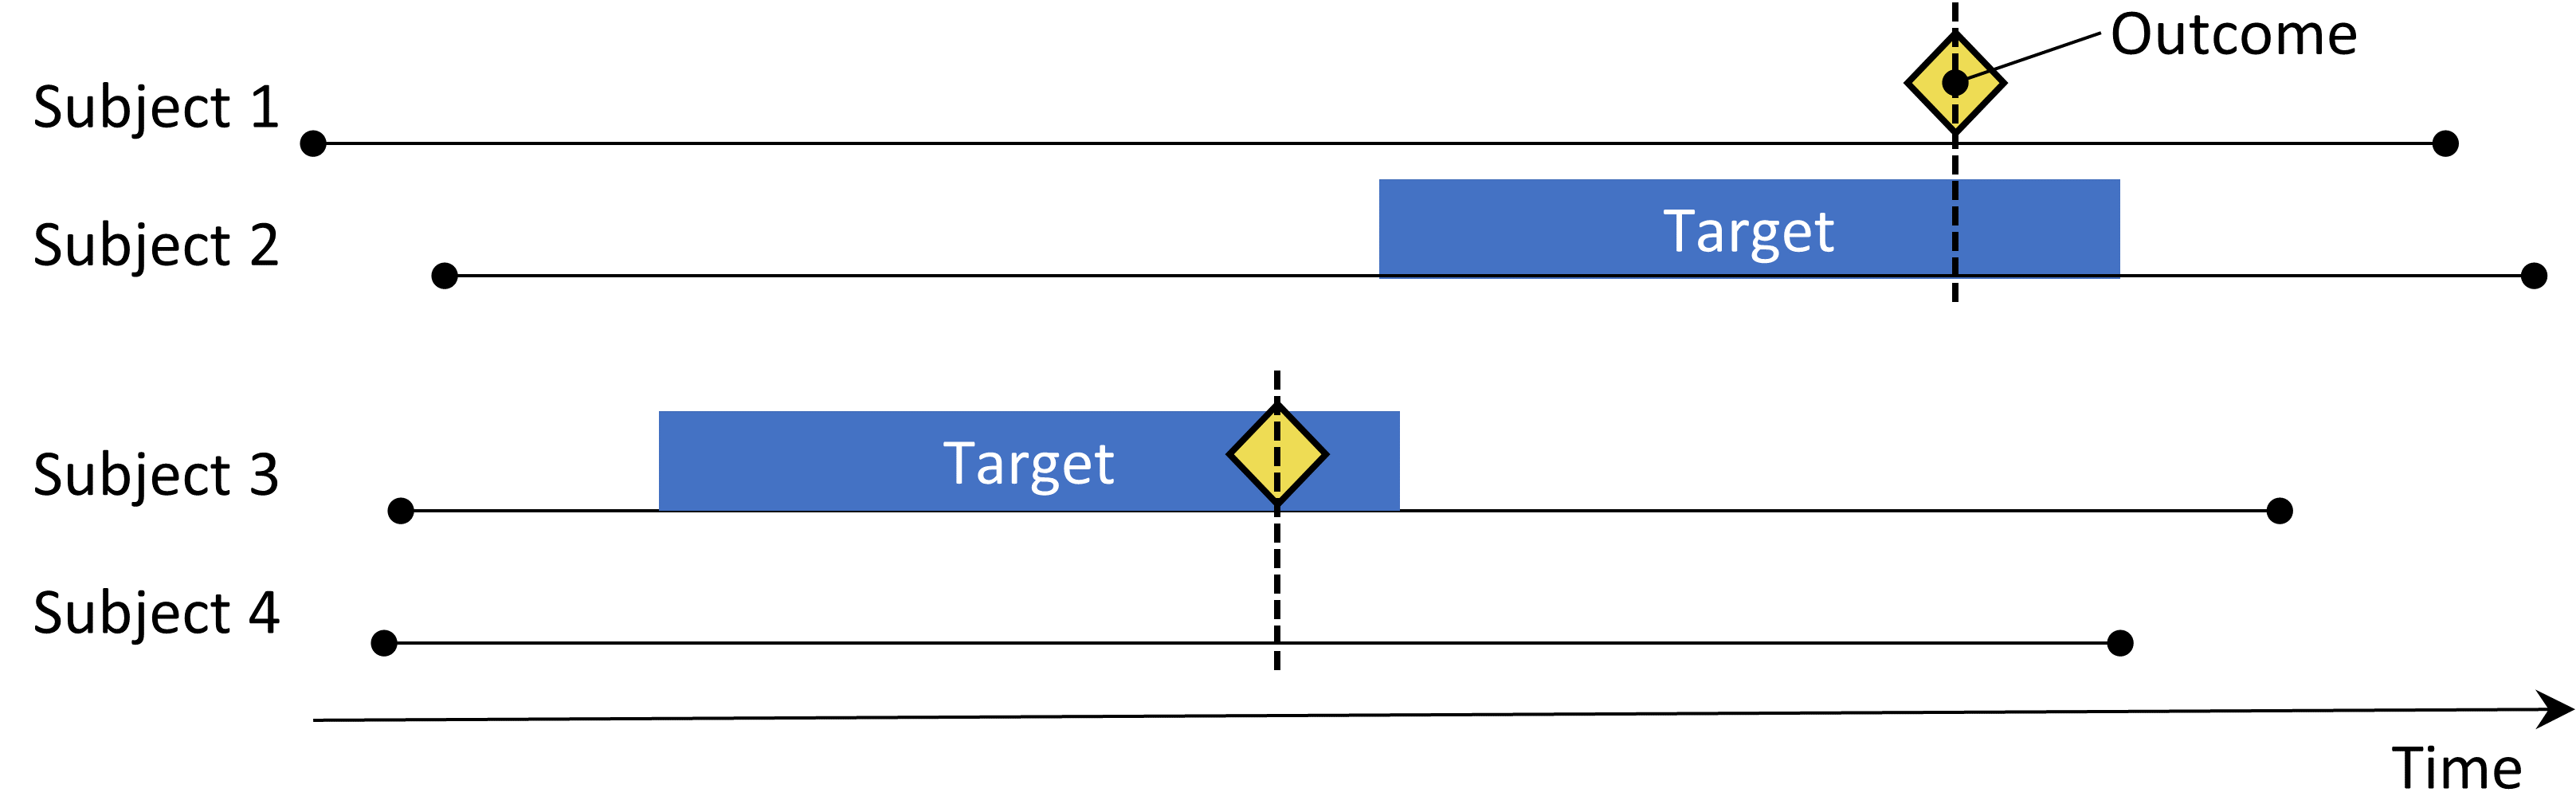
\includegraphics[width=0.9\linewidth]{images/PopulationLevelEstimation/caseControl} 

}

\caption{The case-control design. Subjects with the outcome (‘cases’) are compared to subjects without the outcome (‘controls’) in terms of their exposure status. Often, cases and controls are matched on various characteristics such as age and sex.}\label{fig:caseControl}
\end{figure}

Case-control \citep{vandenbroucke_2012} studies consider the question
``are persons with a specific disease outcome exposed more frequently to
a specific agent than those without the disease?'' Thus, the central
idea is to compare ``cases'', i.e., subjects that experience the outcome
of interest with ``controls'', i.e., subjects that did not experience
the outcome of interest. The choices in Table \ref{tab:ccChoices} define
a case-control question.

\begin{longtable}[]{@{}ll@{}}
\caption{\label{tab:ccChoices} Main design choices in a case-control
design.}\tabularnewline
\toprule
\begin{minipage}[b]{0.23\columnwidth}\raggedright\strut
Choice\strut
\end{minipage} & \begin{minipage}[b]{0.71\columnwidth}\raggedright\strut
Description\strut
\end{minipage}\tabularnewline
\midrule
\endfirsthead
\toprule
\begin{minipage}[b]{0.23\columnwidth}\raggedright\strut
Choice\strut
\end{minipage} & \begin{minipage}[b]{0.71\columnwidth}\raggedright\strut
Description\strut
\end{minipage}\tabularnewline
\midrule
\endhead
\begin{minipage}[t]{0.23\columnwidth}\raggedright\strut
Outcome cohort\strut
\end{minipage} & \begin{minipage}[t]{0.71\columnwidth}\raggedright\strut
A cohort representing the cases (the outcome of interest)\strut
\end{minipage}\tabularnewline
\begin{minipage}[t]{0.23\columnwidth}\raggedright\strut
Control selection\strut
\end{minipage} & \begin{minipage}[t]{0.71\columnwidth}\raggedright\strut
A strategy for selecting controls and their index date\strut
\end{minipage}\tabularnewline
\begin{minipage}[t]{0.23\columnwidth}\raggedright\strut
Target cohort\strut
\end{minipage} & \begin{minipage}[t]{0.71\columnwidth}\raggedright\strut
A cohort representing the treatment\strut
\end{minipage}\tabularnewline
\begin{minipage}[t]{0.23\columnwidth}\raggedright\strut
{[}Nesting cohort{]}\strut
\end{minipage} & \begin{minipage}[t]{0.71\columnwidth}\raggedright\strut
Optionally, a cohort defining the subpopulation from which cases and
controls are drawn\strut
\end{minipage}\tabularnewline
\begin{minipage}[t]{0.23\columnwidth}\raggedright\strut
Time-at-risk\strut
\end{minipage} & \begin{minipage}[t]{0.71\columnwidth}\raggedright\strut
At what time (often relative to the index date) do we consider exposure
status?\strut
\end{minipage}\tabularnewline
\bottomrule
\end{longtable}

Often, one matches controls to cases based on characteristics such as
age and sex to make them more comparable. Another widespread practice is
to nest the analysis within a specific subgroup of people, for example
people that have all been diagnosed with one of the indications of the
exposure of interest.

\subsection{Case-crossover}\label{case-crossover}

\begin{figure}

{\centering 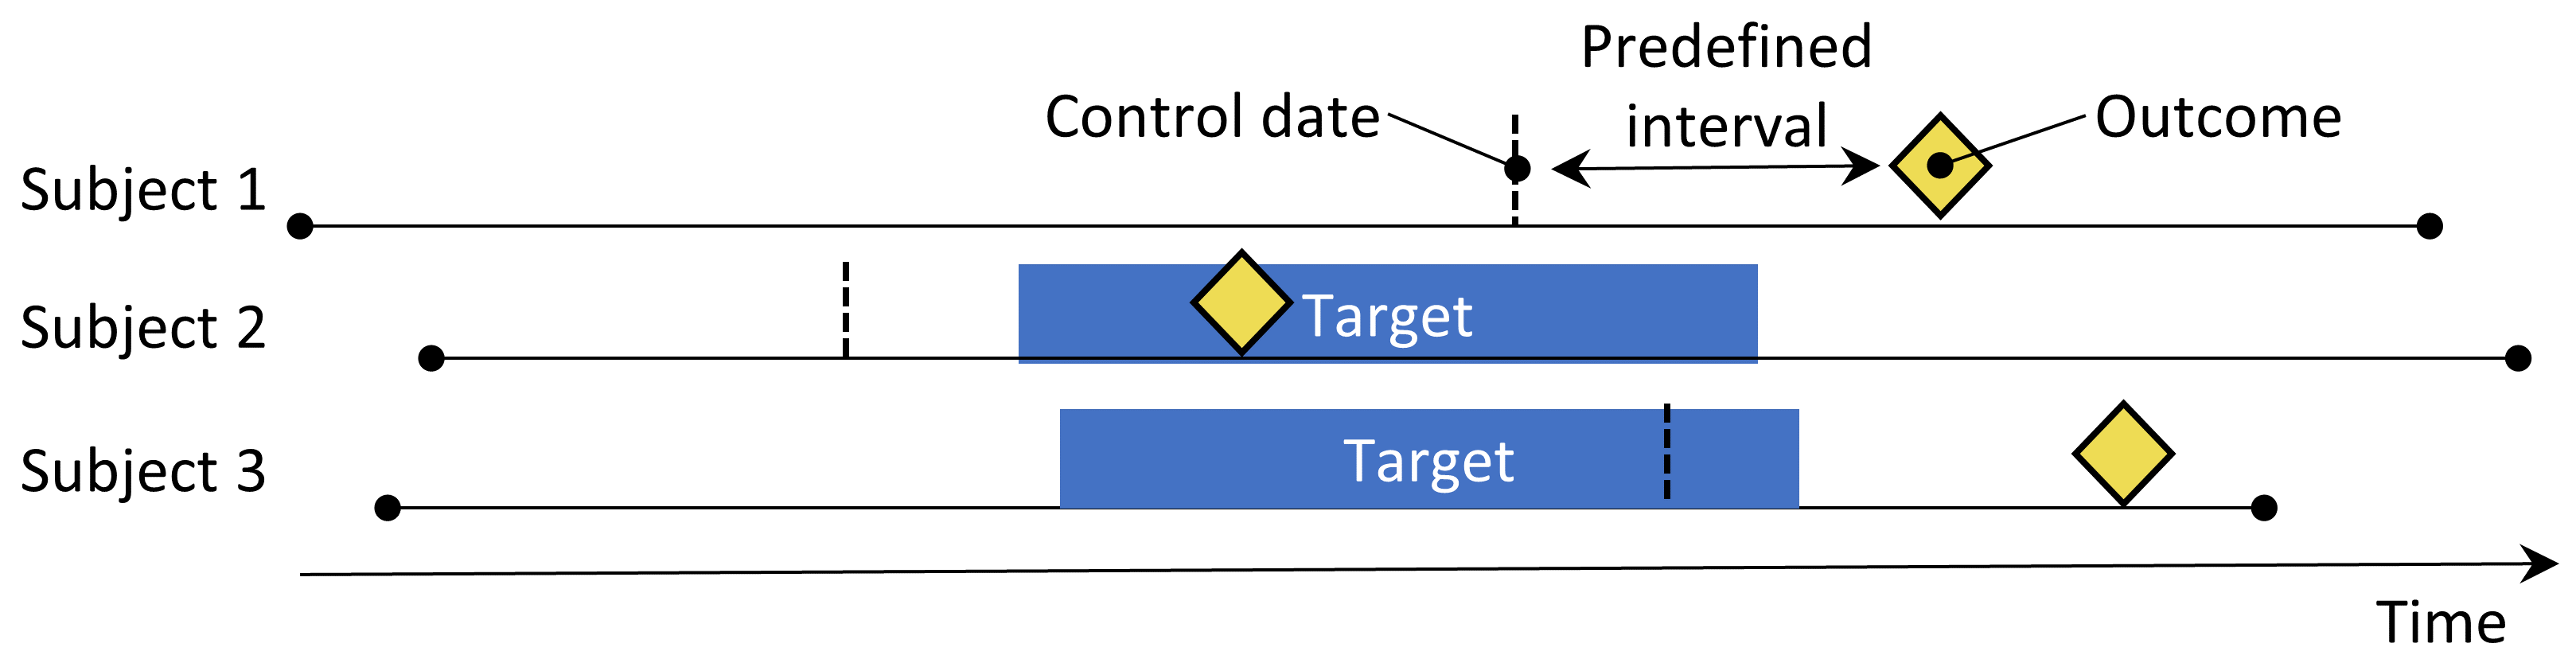
\includegraphics[width=0.9\linewidth]{images/PopulationLevelEstimation/caseCrossover} 

}

\caption{The case-crossover design. The time around the outcome is compared to a control date set at a predefined interval prior to the outcome date.}\label{fig:caseCrossover}
\end{figure}

The case-crossover \citep{maclure_1991} design evaluates whether the
rate of exposure is different at the time of the outcome than at some
predefined number of days prior to the outcome. It is trying to
determine whether there is something special about the day the outcome
occurred. Table \ref{tab:ccrChoices} shows the choices that define a
case-crosover question:

\begin{longtable}[]{@{}ll@{}}
\caption{\label{tab:ccrChoices} Main design choices in a case-crossover
design.}\tabularnewline
\toprule
\begin{minipage}[b]{0.23\columnwidth}\raggedright\strut
Choice\strut
\end{minipage} & \begin{minipage}[b]{0.71\columnwidth}\raggedright\strut
Description\strut
\end{minipage}\tabularnewline
\midrule
\endfirsthead
\toprule
\begin{minipage}[b]{0.23\columnwidth}\raggedright\strut
Choice\strut
\end{minipage} & \begin{minipage}[b]{0.71\columnwidth}\raggedright\strut
Description\strut
\end{minipage}\tabularnewline
\midrule
\endhead
\begin{minipage}[t]{0.23\columnwidth}\raggedright\strut
Outcome cohort\strut
\end{minipage} & \begin{minipage}[t]{0.71\columnwidth}\raggedright\strut
A cohort representing the cases (the outcome of interest)\strut
\end{minipage}\tabularnewline
\begin{minipage}[t]{0.23\columnwidth}\raggedright\strut
Target cohort\strut
\end{minipage} & \begin{minipage}[t]{0.71\columnwidth}\raggedright\strut
A cohort representing the treatment\strut
\end{minipage}\tabularnewline
\begin{minipage}[t]{0.23\columnwidth}\raggedright\strut
Time-at-risk\strut
\end{minipage} & \begin{minipage}[t]{0.71\columnwidth}\raggedright\strut
At what time (often relative to the index date) do we consider exposure
status?\strut
\end{minipage}\tabularnewline
\begin{minipage}[t]{0.23\columnwidth}\raggedright\strut
Control time\strut
\end{minipage} & \begin{minipage}[t]{0.71\columnwidth}\raggedright\strut
The time period used as the control time\strut
\end{minipage}\tabularnewline
\bottomrule
\end{longtable}

Since cases serve as their own control, it is a self-controlled design,
and should therefore be robust to confounding due to between-person
differences. One concern is that, because the outcome date is always
later than the control date, the method will be positively biased if the
overall frequency of exposure increases over time (or negatively biased
if there is a decrease). To address this, the case-time-control design
\citep{suissa_1995} was developed, which adds matched controls to the
case-crossover design to adjust for exposure trends.

\subsection{Self-controlled case
series}\label{self-controlled-case-series}

\begin{figure}

{\centering 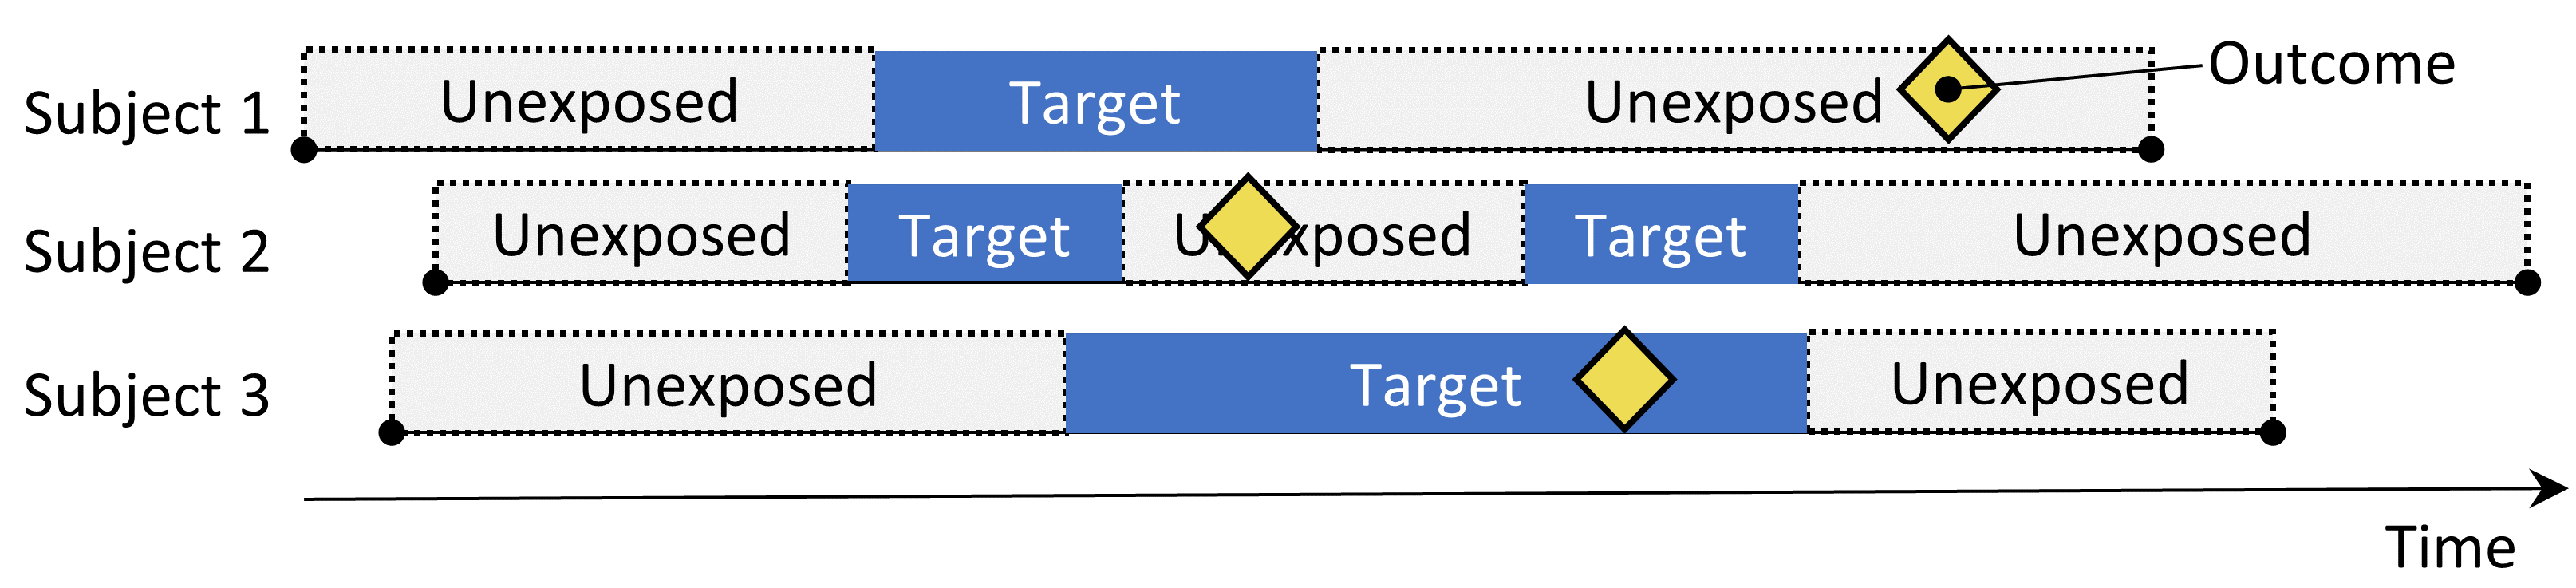
\includegraphics[width=0.9\linewidth]{images/PopulationLevelEstimation/selfControlledCaseSeries} 

}

\caption{The Self-Controlled Case Series design. The rate of outcomes during exposure is compared to the rate of outcomes when not exposed.}\label{fig:selfControlledCaseSeries}
\end{figure}

The Self-Controlled Case Series (SCCS) design
\citep[whitaker\_2006]{farrington_1995} compares the rate of outcomes
during exposure to the rate of outcomes during all unexposed time, both
before, between, and after exposures. It is a Poisson regression that is
conditioned on the person. Thus, it seeks to answer the question:
``Given that a patient has the outcome, is the outcome more likely
during exposed time compared to non-exposed time?''. The choices in
Table \ref{tab:sccsChoices} define an SCCS question.

\begin{longtable}[]{@{}ll@{}}
\caption{\label{tab:sccsChoices} Main design choices in a self-controlled
case series design.}\tabularnewline
\toprule
\begin{minipage}[b]{0.23\columnwidth}\raggedright\strut
Choice\strut
\end{minipage} & \begin{minipage}[b]{0.71\columnwidth}\raggedright\strut
Description\strut
\end{minipage}\tabularnewline
\midrule
\endfirsthead
\toprule
\begin{minipage}[b]{0.23\columnwidth}\raggedright\strut
Choice\strut
\end{minipage} & \begin{minipage}[b]{0.71\columnwidth}\raggedright\strut
Description\strut
\end{minipage}\tabularnewline
\midrule
\endhead
\begin{minipage}[t]{0.23\columnwidth}\raggedright\strut
Target cohort\strut
\end{minipage} & \begin{minipage}[t]{0.71\columnwidth}\raggedright\strut
A cohort representing the treatment\strut
\end{minipage}\tabularnewline
\begin{minipage}[t]{0.23\columnwidth}\raggedright\strut
Outcome cohort\strut
\end{minipage} & \begin{minipage}[t]{0.71\columnwidth}\raggedright\strut
A cohort representing the outcome of interest\strut
\end{minipage}\tabularnewline
\begin{minipage}[t]{0.23\columnwidth}\raggedright\strut
Time-at-risk\strut
\end{minipage} & \begin{minipage}[t]{0.71\columnwidth}\raggedright\strut
At what time (often relative to the target cohort start and end dates)
do we consider the risk of the outcome?\strut
\end{minipage}\tabularnewline
\begin{minipage}[t]{0.23\columnwidth}\raggedright\strut
Model\strut
\end{minipage} & \begin{minipage}[t]{0.71\columnwidth}\raggedright\strut
The model to estimate the effect, including any adjustments for
time-varying confounders\strut
\end{minipage}\tabularnewline
\bottomrule
\end{longtable}

Like other self-controlled designs, the SCCS is robust to confounding
due to between-person differences, but vulnerable to confounding due to
time-varying effects. Several adjustments are possible to attempt to
account for these, for example by including age and season. A special
variant of the SCCS includes not just the exposure of interest, but all
other exposures to drugs recorded in the database \citep{simpson_2013},
potentially adding thousands of additional variables to the model.
L1-regularization using cross-validation to select the regularization
hyperparameter is applied to the coefficients of all exposures except
the exposure of interest.

One important assumption underlying the SCCS is that the observation
period end is independent of the date of the outcome. Because for some
outcomes, especially ones that can be fatal such as stroke, this
assumption can be violated an extension to the SCCS has been developed
that corrects for any such dependency. \citep{farrington_2011}

\section{Designing a hypertension
study}\label{designing-a-hypertension-study}

Describe case study: risk of angioedema and AMI in new users of ACE
inhibitors compared to new users of thiazide and thiazide-like diuretics

\subsection{Implementation the study using
R}\label{implementation-the-study-using-r}

\subsection{Implementation the study using
ATLAS}\label{implementation-the-study-using-atlas}

\section{Advanced topics}\label{advanced-topics}

Best practices:
\url{http://www.ohdsi.org/web/wiki/doku.php?id=development:best_practices_estimation}

Negative and positive controls, empirical calibration

\section{Excercises}\label{excercises}

\chapter{Patient Level Prediction}\label{PatientLevelPrediction}

\emph{Chapter leads: Peter Rijnbeek \& Jenna Reps}

Clinical decision making is a complicated task in which the clinician
has to infer a diagnosis or treatment pathway based on the available
medical history of the patient and the current clinical guidelines.
Clinical prediction models have been developed to support this decision
making process and are used in clinical practice in a wide spectrum of
specialties. These models predict a diagnostic or prognostic outcome
based on a combination of patient characteristics, e.g.~demographic
information, disease history, treatment history. The number of
publications describing clinical prediction models has increased
strongly over the last 10 years. An example is the Garvan model that
predicts the 5-years and 10-years fractures risk in any elderly man or
woman based on age, fracture history, fall history, bone mass density or
weight \citep{nguyen2008}. Many prediction models have been developed in
patient subgroups at higher risk that need more intensive monitoring,
e.g.~the prediction of 30-day mortality after an acute myocardial
described by \citet{lee1995}. Also, many models have been developed for
asymptomatic subjects in the population, e.g.~the famous Framingham risk
functions for cardiovascular disease \citep{wilson1998}, or the models
for breast cancer screening \citep{engel2015}.

Surprisingly, most currently used models are estimated using small
datasets and contain a limited set of patient characteristics. For
example, in a review of 102 prognostic models in traumatic brain injury
showed that three quarters of the models were based on samples with less
than 500 patients \citep{perel2006}. This low sample size, and thus low
statistical power, forces the data analyst to make stronger modelling
assumptions. The selection of the often limited set of patient
characteristics is strongly guided by the expert knowledge at hand. This
contrasts sharply with the reality of modern medicine wherein patients
generate a rich digital trail, which is well beyond the power of any
medical practitioner to fully assimilate. Presently, health care is
generating huge amount of patient-specific information contained in the
Electronic Health Record (EHR). This includes structured data in the
form of diagnose, medication, laboratory test results, and unstructured
data contained in clinical narratives. Currently, it is unknown how much
predictive accuracy can be gained by leveraging the large amount of data
originating from the complete EHR of a patient.

Massive-scale, patient-specific predictive modeling has become reality
due the OHDSI initiative in which the common data model (CDM) allows for
uniform and transparent analysis at an unprecedented scale. These large
standardized populations contain rich data to build highly predictive
large-scale models and also provide immediate opportunity to serve large
communities of patients who are in most need of improved quality of
care. Such models can inform truly personalized medical care leading
hopefully to sharply improved patient outcomes. Furthermore, these
models could assist in the design and analysis of randomized controlled
trials (RCT) by enabling a better patient stratification or can be
utilized to adjust for confounding variables in observational research.
More accurate prediction models contribute to targeting of treatment and
to increasing cost-effectiveness of medical care.

Advances in machine learning for large dataset analysis have led to
increased interest in applying patient-level prediction on this type of
data. However, many published efforts in patient-level-prediction do not
follow the model development guidelines, fail to perform extensive
external validation, or provide insufficient model details that limits
the ability of independent researchers to reproduce the models and
perform external validation. This makes it hard to fairly evaluate the
predictive performance of the models and reduces the likelihood of the
model being used appropriately in clinical practice. To improve
standards, several papers have been written detailing guidelines for
best practices in developing and reporting prediction models.

The Transparent Reporting of a multivariable prediction model for
Individual Prognosis Or Diagnosis (TRIPOD) statement \footnote{\url{https://www.equator-network.org/reporting-guidelines/tripod-statement/}}
provides clear recommendations for reporting prediction model
development and validation and addresses some of the concerns related to
transparency. However, data structure heterogeneity and inconsistent
terminologies still make collaboration and model sharing difficult as
different researchers are often required to write new code to extract
the data from their databases and may define variables differently.

In our paper \citep{reps2018}, we propose a standardised framework for
patient-level prediction that utilizes the OMOP Common Data Model (CDM)
and standardized vocabularies, and describe the open-source software
that we developed implementing the framework's pipeline. The framework
is the first to support existing best practice guidelines and will
enable open dissemination of models that can be extensively validated
across the network of OHDSI collaborators.

Figure \ref{fig:figure1}, illustrates the prediction problem we address.
Among a population at risk, we aim to predict which patients at a
defined moment in time (t = 0) will experience some outcome during a
time-at-risk. Prediction is done using only information about the
patients in an observation window prior to that moment in time.

\begin{figure}
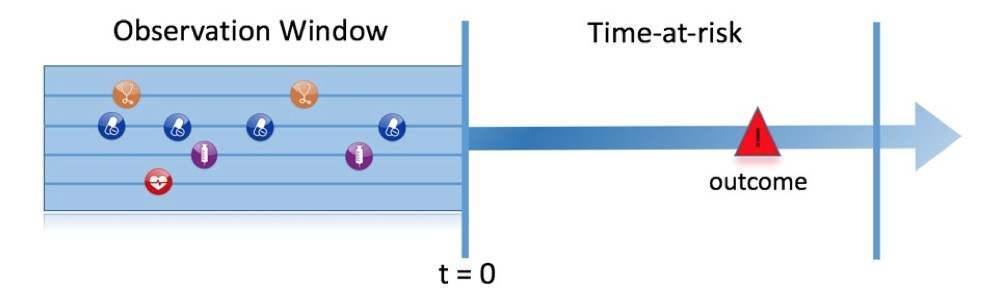
\includegraphics[width=1\linewidth]{images/PatientLevelPrediction/Figure1} \caption{The prediction problem.}\label{fig:figure1}
\end{figure}

As shown in Table \ref{tab:plpDesign}, to define a prediction problem we
have to define t=0 by a target Cohort (T), the outcome we like to
predict by an outcome cohort (O), and the time-at-risk (TAR).
Furthermore, we have to make design choices for the model we like to
develop, and determine the observational datasets to perform internal
and external validation.

\begin{longtable}[]{@{}ll@{}}
\caption{\label{tab:plpDesign} Main design choices in a prediction
design.}\tabularnewline
\toprule
\begin{minipage}[b]{0.23\columnwidth}\raggedright\strut
Choice\strut
\end{minipage} & \begin{minipage}[b]{0.71\columnwidth}\raggedright\strut
Description\strut
\end{minipage}\tabularnewline
\midrule
\endfirsthead
\toprule
\begin{minipage}[b]{0.23\columnwidth}\raggedright\strut
Choice\strut
\end{minipage} & \begin{minipage}[b]{0.71\columnwidth}\raggedright\strut
Description\strut
\end{minipage}\tabularnewline
\midrule
\endhead
\begin{minipage}[t]{0.23\columnwidth}\raggedright\strut
Target cohort\strut
\end{minipage} & \begin{minipage}[t]{0.71\columnwidth}\raggedright\strut
A cohort for whom we wish to predict\strut
\end{minipage}\tabularnewline
\begin{minipage}[t]{0.23\columnwidth}\raggedright\strut
Outcome cohort\strut
\end{minipage} & \begin{minipage}[t]{0.71\columnwidth}\raggedright\strut
A cohort representing the outcome we wish to predict\strut
\end{minipage}\tabularnewline
\begin{minipage}[t]{0.23\columnwidth}\raggedright\strut
Time-at-risk\strut
\end{minipage} & \begin{minipage}[t]{0.71\columnwidth}\raggedright\strut
For what time relative to t=0 do we want to make the prediction?\strut
\end{minipage}\tabularnewline
\begin{minipage}[t]{0.23\columnwidth}\raggedright\strut
Model\strut
\end{minipage} & \begin{minipage}[t]{0.71\columnwidth}\raggedright\strut
What algorithms using which parameters do we want use, and what
predictor variables do we want to include?\strut
\end{minipage}\tabularnewline
\bottomrule
\end{longtable}

This conceptual framework works for all type of prediction problems:

\begin{itemize}
\tightlist
\item
  Disease onset and progression

  \begin{itemize}
  \tightlist
  \item
    \textbf{Structure}: Amongst patients who are newly diagnosed with
    \emph{{[}a disease{]}}, who will go on to have \emph{{[}another
    disease or complication{]}} within \emph{{[}time horizon from
    diagnosis{]}}?
  \item
    \textbf{Example}: Among newly diagnosed atrial fibrilation patients,
    who will go on to have ischemic stroke in the next three years?
  \end{itemize}
\item
  Treatment choice

  \begin{itemize}
  \tightlist
  \item
    \textbf{Structure}: Amongst patients with \emph{{[}indicated
    disease{]}} who are treated with either \emph{{[}treatment 1{]}} or
    \emph{{[}treatment 2{]}}, which patients were treated with
    \emph{{[}treatment 1{]}} (on day 0).
  \item
    \textbf{Example}: Among patients with atrial fibrilation who took
    either warfarin or rivaroxaban, which patients gets warfarin?
    (e.g.~for a propensity model)
  \end{itemize}
\item
  Treatment response

  \begin{itemize}
  \tightlist
  \item
    \textbf{Structure}: Amongst new users of \emph{{[}a treatment{]}},
    who will experience \emph{{[}some effect{]}} in \emph{{[}time
    window{]}} ?
  \item
    \textbf{Example}: Which patients with diabetes who start on
    metformin stay on metform for three years?
  \end{itemize}
\item
  Treatment safety

  \begin{itemize}
  \tightlist
  \item
    \textbf{Structure}: Amongst new users of \emph{{[}a treatment{]}},
    who will experience \emph{{[}adverse event{]}} in \emph{{[}time
    window{]}}?
  \item
    \textbf{Example}: Amongst new users of warfarin, who will have a GI
    bleed in one year?
  \end{itemize}
\item
  Treatment adherence

  \begin{itemize}
  \tightlist
  \item
    \textbf{Structure}: Amongst new users of \emph{{[}a treatment{]}},
    who will achieve \emph{{[}adherence metric{]}} at \emph{{[}time
    window{]}}?
  \item
    \textbf{Example}: Which patients with diabetes who start on
    metformin achieve \textgreater{}=80\% proportion of days covered at
    one year?
  \end{itemize}
\end{itemize}

In the next sections we will explain the best practices for model
specification, implementation, and evaluation using OHDSI's
Patient-Level Prediction (PLP) framework as guidance.

\section{Designing a hypertension
study}\label{designing-a-hypertension-study-1}

The first step is to clearly define the prediction problem.
Interestingly, in many published papers the prediction problem is poorly
defined, e.g.~it is unclear how the index date (start of the target
Cohort) is defined. A poorly defined prediction problem does not allow
for external validation by others let alone implementation in clinical
practice. In the PLP framework we have enforced that we have to define
the prediction problem we like to address, in which population we will
build the model, which model we will build and how we will evaluate its
performance. In this section we will guide you through this process and
we will use a ``Disease onset and progression'' prediction type as an
example.

\subsection{Problem definition}\label{problem-definition}

Atrial fibrillation is a disease characterized by an irregular heart
rate that can cause poor blood flow. Patients with atrial fibrillation
are at increased risk of ischemic stroke. Anticoagulation is a
recommended prophylaxis treatment strategy for patients at high risk of
stroke, though the underuse of anticoagulants and persistent severity of
ischemic stroke represents a substantial unmet medical need. Various
strategies have been developed to predict risk of ischemic stroke in
patients with atrial fibrillation. CHADS2 \citep{gage2001} was developed
as a risk score based on history of congestive heart failure,
hypertension, age\textgreater{}=75, diabetes and stroke. CHADS2 was
initially derived using Medicare claims data, where it achieved good
discrimination (AUC=0.82). However, subsequent external validation
studies revealed the CHADS2 had substantially lower predictive accuracy
\citep{keogh2011}. Subsequent stroke risk calculators have been
developed and evaluated, including the extension of CHADS2Vasc. The
management of atrial fibrillation has evolved substantially over the
last decade, for various reasons that include the introduction of novel
oral anticoagulants. With these innovations has come a renewed interest
in greater precision medicine for stroke prevention.

We will apply the PLP framework to observational healthcare data to
address the following patient-level prediction question:

\begin{quote}
Amongst patients who have just started on an ACE inhibitor for the first
time, who will experience angioedema in the following year?
\end{quote}

\subsection{Study population
definition}\label{study-population-definition}

The final study population in which we will develop our model is often a
subset of the target population, because we will e.g.~apply criteria
that are dependent on T and O or we want to do sensitivity analyses with
subpopulations of T. For this we have to answer the following questions:

\begin{itemize}
\item
  \emph{What is the minimum amount of observation time we require before
  the start of the target cohort?} This choice could depend on the
  available patient time in your training data, but also on the time you
  expect to be available in the data sources you want to apply the model
  on in the future. The longer the minimum observation time, the more
  baseline history time is available for each person to use for feature
  extraction, but the fewer patients will qualify for analysis.
  Moreover, there could be clinical reasons to choose a short or longer
  lookback period. For our example, we will use a prior history as
  lookback period (washout period).
\item
  \emph{Can patients enter the target cohort multiple times?} In the
  target cohort definition, a person may qualify for the cohort multiple
  times during different spans of time, for example if they had
  different episodes of a disease or separate periods of exposure to a
  medical product. The cohort definition does not necessarily apply a
  restriction to only let the patients enter once, but in the context of
  a particular patient-level prediction problem, a user may want to
  restrict the cohort to the first qualifying episode. In our example, a
  person can only enter the target cohort once since our criteria was
  based on first use of an ACE inhibitor.
\item
  \emph{Do we allow persons to enter the cohort if they experienced the
  outcome before?} Do we allow persons to enter the target cohort if
  they experienced the outcome before qualifying for the target cohort?
  Depending on the particular patient-level prediction problem, there
  may be a desire to predict `incident' first occurrence of an outcome,
  in which case patients who have previously experienced the outcome are
  not `at-risk' for having a first occurrence and therefore should be
  excluded from the target cohort. In other circumstances, there may be
  a desire to predict `prevalent' episodes, whereby patients with prior
  outcomes can be included in the analysis and the prior outcome itself
  can be a predictor of future outcomes. For our prediction example, we
  will choose not to include those with prior angioedema.
\item
  \emph{How do we define the period in which we will predict our outcome
  relative to the target cohort start?} We actually have to make two
  decisions to answer that question. First, does the time-at-risk window
  start at the date of the start of the target cohort or later?
  Arguments to make it start later could be that you want to avoid
  outcomes that were entered late in the record that actually occurred
  before the start of the target cohort or you want to leave a gap where
  interventions to prevent the outcome could theoretically be
  implemented. Second, you need to define the time-at-risk by setting
  the risk window end, as some specification of days offset relative to
  the target cohort start or end dates. For our problem we will predict
  in a `time-at-risk' window starting 1 day after the start of the
  target cohort up to 365 days later.
\item
  \emph{Do we require a minimum amount of time-at-risk?} We have to
  decide if we want to include patients that did not experience the
  outcome but did leave the database earlier than the end of our
  time-at-risk period. These patients may experience the outcome when we
  do not observe them. For our prediction problem we decide to answer
  this question with `Yes, require a mimimum time-at-risk' for that
  reason. Furthermore, we have to decide if this constraint also applies
  to persons who experienced the outcome or we will include all persons
  with the outcome irrespective of their total time at risk. For
  example, if the outcome is death, then persons with the outcome are
  likely censored before the full time-at-risk period is complete.
\end{itemize}

\subsection{Model development
settings}\label{model-development-settings}

To develop the model we have to decide which algorithm(s) we like to
train. We see the selection of the best algorithm for a certain
prediction problem as an empirical question, i.e.~you need to let the
data speak for itself and try different approaches to find the best one.
There is no algorithm that will work best for all problems (no free
lunch). In our framework we therefore aim to implement many algorithms.
Furthermore, we made the system modular so you can add your own custom
algorithms. This out-of-scope for this chapter but mode details can be
found in the \emph{AddingCustomAlgorithms} vignette in the
\href{https://ohdsi.github.io/PatientLevelPrediction/}{PatientLevelPrediction}
package.

Our framework currently contains the following algorithms to choose
from:

\begin{description}
\tightlist
\item[Regularized Logistic Regression]
Lasso logistic regression belongs to the family of generalized linear
models, where a linear combination of the variables is learned and
finally a logistic function maps the linear combination to a value
between 0 and 1. The lasso regularization adds a cost based on model
complexity to the objective function when training the model. This cost
is the sum of the absolute values of the linear combination of the
coefficients. The model automatically performs feature selection by
minimizing this cost. We use the
\href{https://ohdsi.github.io/Cyclops/}{Cyclops} (Cyclic coordinate
descent for logistic, Poisson and survival analysis) package to perform
large-scale regularized logistic regression. \textbf{Hyper-parameters}:
var (starting variance), seed.
\item[Gradient boosting machines]
Gradient boosting machines is a boosting ensemble technique and in our
framework it combines multiple decision trees. Boosting works by
iteratively adding decision trees but adds more weight to the
data-points that are misclassified by prior decision trees in the cost
function when training the next tree. We use Extreme Gradient Boosting,
which is an efficient implementation of the gradient boosting framework
implemented in the xgboost R package available from CRAN.
\textbf{Hyper-parameters}: ntree (number of trees), max depth (max
levels in tree), min rows (minimum data points in in node), learning
rate, seed \textbar{} mtry (number of features in each tree),ntree
(number of trees), maxDepth (max levels in tree), minRows (minimum data
points in in node),balance (balance class labels), seed.
\item[Random forest]
Random forest is a bagging ensemble technique that combines multiple
decision trees. The idea behind bagging is to reduce the likelihood of
overfitting, by using weak classifiers, but combining multiple diverse
weak classifiers into a strong classifier. Random forest accomplishes
this by training multiple decision trees but only using a subset of the
variables in each tree and the subset of variables differ between trees.
Our packages uses the sklearn learn implementation of Random Forest in
python. \textbf{Hyper-parameters}: mtry (number of features in each
tree),ntree (number of trees), maxDepth (max levels in tree), minRows
(minimum data points in in node),balance (balance class labels), seed.
\item[K-nearest neighbors]
K-nearest neighbors (KNN) is an algorithm that uses some metric to find
the K closest labelled data-points, given the specified metric, to a new
unlabelled data-point. The prediction of the new data-points is then the
most prevalent class of the K-nearest labelled data-points. There is a
sharing limitation of KNN, as the model requires labelled data to
perform the prediction on new data, and it is often not possible to
share this data across data sites. We included the
\href{https://github.com/OHDSI/BigKnn}{BigKnn} package developed in
OHDSI which is a large scale k-nearest neighbor classifier.
\textbf{Hyper-parameters}: k (number of neighbours), weighted (weight by
inverse frequency).
\item[Naive Bayes]
The Naive Bayes algorithm applies the Bayes' theorem with the ``naive''
assumption of conditional independence between every pair of features
given the value of the class variable. Based on the likelihood the data
belongs to a class and the prior distribution of the class, a posterior
distribution is obtained. \textbf{Hyper-parameters}: none.
\item[AdaBoost]
AdaBoost is a boosting ensemble technique. Boosting works by iteratively
adding classifiers but adds more weight to the data-points that are
misclassified by prior classifiers in the cost function when training
the next classifier. We use the sklearn ``AdaboostClassifier''
implementation in Python. \textbf{Hyper-parameters}: nEstimators (the
maximum number of estimators at which boosting is terminated),
learningRate (learning rate shrinks the contribution of each classifier
by learning\_rate. There is a trade-off between learningRate and
nEstimators).
\item[Decision Tree]
A decision tree is a classifier that partitions the variable space using
individual tests selected using a greedy approach. It aims to find
partitions that have the highest information gain to separate the
classes. The decision tree can easily overfit by enabling a large number
of partitions (tree depth) and often needs some regularization (e.g.,
pruning or specifying hyper-parameters that limit the complexity of the
model). We use the sklearn ``DecisionTreeClassifier'' implementation in
Python. \textbf{Hyper-parameters}: maxDepth (the maximum depth of the
tree), minSamplesSplit,minSamplesLeaf, minImpuritySplit (threshold for
early stopping in tree growth. A node will split if its impurity is
above the threshold, otherwise it is a leaf.), seed,classWeight
(``Balance''" or ``None'').
\item[Multilayer Perception]
Neural networks containing multiple layers that weight their inputs
using a non-linear function. The first layer is the input layer, the
last layer is the output layer the between are the hidden layers. Neural
networks are generally trained using feed forward back-propagation. This
is when you go through the network with a data-point and calculate the
error between the true label and predicted label, then go backwards
through the network and update the linear function weights based on the
error. \textbf{Hyper-parameters}: size (the number of hidden nodes),
alpha (the l2 regularisation), seed.
\item[Deep Learning]
Deep learning such as deep nets, convolutional neural networks or
recurrent neural networks are similar to a neural network but have
multiple hidden layers that aim to learn latent representations useful
for prediction. In a seperate vignette in the
\href{https://ohdsi.github.io/PatientLevelPrediction/}{PatientLevelPrediction}
package we describe these models and hyper-parameters in more detail.
\end{description}

Furthermore, we have to decide on the \textbf{covariates} that we will
use to train our model. In our example, we like to add gender, age, all
conditions, drugs and drug groups, and visit counts. We also have to
specify in which time windows we will look and we decide to look in year
before and any time prior.

\subsection{Model evaluation}\label{model-evaluation}

Finally, we have to define how we will train and test our model on our
data, i.e.~how we perform \textbf{internal validation}. For this we have
to decide how we divide our dataset in a training and testing dataset
and how we randomly assign patients to these two sets. Dependent on the
size of the training set we can decide how much data we like to use for
training, typically this is a 75\% - 25\% split. If you have very large
datasets you can use more data for training. To randomly assign patients
to the training and testing set, there are two commonly used approaches:

\begin{enumerate}
\def\labelenumi{\arabic{enumi}.}
\tightlist
\item
  split by person. In this case a random seed is used to assign the
  patient to either sets.
\item
  split by time. In this case a time point is used to split the persons,
  e.g.~75\% of the data is before and 25\% is after this date. The
  advantage of this is that you take into consideration that the health
  care system has changed over time.
\end{enumerate}

For our prediction model we decide to start with a Regularized Logistic
Regression and will use the default parameters. We will do a 75\%-25\%
split by person.

\subsection{Study summary}\label{study-summary}

We now completely defined our study as shown in Table
\ref{tab:plpSummary}.

\begin{longtable}[]{@{}ll@{}}
\caption{\label{tab:plpSummary} Main design choices for our
study.}\tabularnewline
\toprule
\begin{minipage}[b]{0.23\columnwidth}\raggedright\strut
Choice\strut
\end{minipage} & \begin{minipage}[b]{0.71\columnwidth}\raggedright\strut
Description\strut
\end{minipage}\tabularnewline
\midrule
\endfirsthead
\toprule
\begin{minipage}[b]{0.23\columnwidth}\raggedright\strut
Choice\strut
\end{minipage} & \begin{minipage}[b]{0.71\columnwidth}\raggedright\strut
Description\strut
\end{minipage}\tabularnewline
\midrule
\endhead
\begin{minipage}[t]{0.23\columnwidth}\raggedright\strut
Target cohort\strut
\end{minipage} & \begin{minipage}[t]{0.71\columnwidth}\raggedright\strut
Patients who have just started on an ACE inhibitor for the first
time.\strut
\end{minipage}\tabularnewline
\begin{minipage}[t]{0.23\columnwidth}\raggedright\strut
Outcome cohort\strut
\end{minipage} & \begin{minipage}[t]{0.71\columnwidth}\raggedright\strut
Angioedema.\strut
\end{minipage}\tabularnewline
\begin{minipage}[t]{0.23\columnwidth}\raggedright\strut
Time-at-risk\strut
\end{minipage} & \begin{minipage}[t]{0.71\columnwidth}\raggedright\strut
1 day till 365 days from cohort start. We will require at least 364 days
at risk.\strut
\end{minipage}\tabularnewline
\begin{minipage}[t]{0.23\columnwidth}\raggedright\strut
Model\strut
\end{minipage} & \begin{minipage}[t]{0.71\columnwidth}\raggedright\strut
Gradient Boosting Machine with hyper-parameters ntree: 5000, max depth:
4 or 7 or 10 and learning rate: 0.001 or 0.01 or 0.1 or 0.9. Covariates
will include gender, age, conditions, drugs, drug groups, and visit
count. Data split: 75\% train - 25\% test, randomly assigned by
person.\strut
\end{minipage}\tabularnewline
\bottomrule
\end{longtable}

We define the target cohort as the first exposure to any ACE inhibitor.
Patients are excluded if they have less than 365 days of prior
observation time or have prior angioedema.

\section{Implementing the study in R}\label{implementing-the-study-in-r}

Now we have completely designed our study we have to implement the
study. This will be done using the
\href{https://ohdsi.github.io/PatientLevelPrediction/}{PatientLevelPrediction}
package to build patient-level predictive models. The package enables
data extraction, model building, and model evaluation using data from
databases that are translated into the OMOP CDM.

\subsection{Cohort instantiation}\label{cohort-instantiation}

We first need to instantiate the target and outcome cohorts.
Instantiating cohorts is described in Chapter \ref{Cohorts}. The
Appendix provides the full definitions of the target (Appendix
\ref{AceInhibitors}) and outcome (Appendix \ref{Angioedema}) cohorts. In
this example we will assume the ACE inhibitors cohort has ID 1, and the
angioedema cohort has ID 2.

\subsection{Data extraction}\label{data-extraction}

We first need to tell R how to connect to the server.
\href{https://ohdsi.github.io/PatientLevelPrediction/}{\texttt{PatientLevelPrediction}}
uses the
\href{https://ohdsi.github.io/DatabaseConnector/}{\texttt{DatabaseConnector}}
package, which provides a function called
\texttt{createConnectionDetails}. Type \texttt{?createConnectionDetails}
for the specific settings required for the various database management
systems (DBMS). For example, one might connect to a PostgreSQL database
using this code:

\begin{Shaded}
\begin{Highlighting}[]
\KeywordTok{library}\NormalTok{(PatientLevelPrediction)}
\NormalTok{connDetails <-}\StringTok{ }\KeywordTok{createConnectionDetails}\NormalTok{(}\DataTypeTok{dbms =} \StringTok{"postgresql"}\NormalTok{,}
                                       \DataTypeTok{server =} \StringTok{"localhost/ohdsi"}\NormalTok{,}
                                       \DataTypeTok{user =} \StringTok{"joe"}\NormalTok{,}
                                       \DataTypeTok{password =} \StringTok{"supersecret"}\NormalTok{)}

\NormalTok{cdmDbSchema <-}\StringTok{ "my_cdm_data"}
\NormalTok{cohortsDbSchema <-}\StringTok{ "scratch"}
\NormalTok{cohortsDbTable <-}\StringTok{ "my_cohorts"}
\NormalTok{cdmVersion <-}\StringTok{ "5"}
\end{Highlighting}
\end{Shaded}

The last four lines define the \texttt{cdmDbSchema},
\texttt{cohortsDbSchema}, and \texttt{cohortsDbTable} variables, as well
as the CDM version. We will use these later to tell R where the data in
CDM format live, where the cohorts of interest have been created, and
what version CDM is used. Note that for Microsoft SQL Server, database
schemas need to specify both the database and the schema, so for example
\texttt{cdmDbSchema\ \textless{}-\ "my\_cdm\_data.dbo"}.

First it makes sense to verify that the cohort creation has succeeded,
by counting the number of cohort entries:

\begin{Shaded}
\begin{Highlighting}[]
\NormalTok{sql <-}\StringTok{ }\KeywordTok{paste}\NormalTok{(}\StringTok{"SELECT cohort_definition_id, COUNT(*) AS count"}\NormalTok{,}
\StringTok{"FROM @cohortsDbSchema.cohortsDbTable"}\NormalTok{,}
\StringTok{"GROUP BY cohort_definition_id"}\NormalTok{)}
\NormalTok{conn <-}\StringTok{ }\KeywordTok{connect}\NormalTok{(connDetails)}
\KeywordTok{renderTranslateQuerySql}\NormalTok{(}\DataTypeTok{connection =}\NormalTok{ conn, }
                        \DataTypeTok{sql =}\NormalTok{ sql,}
                        \DataTypeTok{cohortsDbSchema =}\NormalTok{ cohortsDbSchema,}
                        \DataTypeTok{cohortsDbTable =}\NormalTok{ cohortsDbTable)}
\end{Highlighting}
\end{Shaded}

\begin{verbatim}
##   cohort_definition_id  count
## 1                    1 527616
## 2                    2   3201
\end{verbatim}

Now we can tell
\href{https://ohdsi.github.io/PatientLevelPrediction/}{PatientLevelPrediction}
to extract all necessary data for our analysis. Covariates are extracted
using the
\href{https://ohdsi.github.io/FeatureExtraction/}{\texttt{FeatureExtraction}}
package. For more detailed information on the FeatureExtraction package
see its vignettes. For our example study we decided to use these
settings:

\begin{Shaded}
\begin{Highlighting}[]
\NormalTok{covSettings <-}\StringTok{ }\KeywordTok{createCovariateSettings}\NormalTok{(}\DataTypeTok{useDemographicsGender =} \OtherTok{TRUE}\NormalTok{,}
                                       \DataTypeTok{useDemographicsAge =} \OtherTok{TRUE}\NormalTok{,}
                                       \DataTypeTok{useConditionGroupEraLongTerm =} \OtherTok{TRUE}\NormalTok{,}
                                       \DataTypeTok{useConditionGroupEraAnyTimePrior =} \OtherTok{TRUE}\NormalTok{,}
                                       \DataTypeTok{useDrugGroupEraLongTerm =} \OtherTok{TRUE}\NormalTok{,}
                                       \DataTypeTok{useDrugGroupEraAnyTimePrior =} \OtherTok{TRUE}\NormalTok{,}
                                       \DataTypeTok{useVisitConceptCountLongTerm =} \OtherTok{TRUE}\NormalTok{,}
                                       \DataTypeTok{longTermStartDays =} \OperatorTok{-}\DecValTok{365}\NormalTok{,}
                                       \DataTypeTok{endDays =} \OperatorTok{-}\DecValTok{1}\NormalTok{)}
\end{Highlighting}
\end{Shaded}

The final step for extracting the data is to run the \texttt{getPlpData}
function and input the connection details, the database schema where the
cohorts are stored, the cohort definition ids for the cohort and
outcome, and the washoutPeriod which is the minimum number of days prior
to cohort index date that the person must have been observed to be
included into the data, and finally input the previously constructed
covariate settings.

\begin{Shaded}
\begin{Highlighting}[]
\NormalTok{plpData <-}\StringTok{ }\KeywordTok{getPlpData}\NormalTok{(}\DataTypeTok{connectionDetails =}\NormalTok{ connDetails,}
                      \DataTypeTok{cdmDatabaseSchema =}\NormalTok{ cdmDbSchema,}
                      \DataTypeTok{cohortDatabaseSchema =}\NormalTok{ cohortsDbSchema,}
                      \DataTypeTok{cohortTable =}\NormalTok{ cohortsDbSchema,}
                      \DataTypeTok{cohortId =} \DecValTok{1}\NormalTok{,}
                      \DataTypeTok{covariateSettings =}\NormalTok{ covariateSettings,}
                      \DataTypeTok{outcomeDatabaseSchema =}\NormalTok{ cohortsDbSchema,}
                      \DataTypeTok{outcomeTable =}\NormalTok{ cohortsDbSchema,}
                      \DataTypeTok{outcomeIds =} \DecValTok{2}\NormalTok{,}
                      \DataTypeTok{sampleSize =} \DecValTok{10000}
\NormalTok{)}
\end{Highlighting}
\end{Shaded}

There are many additional parameters for the \texttt{getPlpData}
function which are all documented in the
\href{https://ohdsi.github.io/PatientLevelPrediction/}{PatientLevelPrediction}
manual. The resulting \texttt{plpData} object uses the package
\texttt{ff} to store information in a way that ensures R does not run
out of memory, even when the data are large.

Creating the \texttt{plpData} object can take considerable computing
time, and it is probably a good idea to save it for future sessions.
Because \texttt{plpData} uses \texttt{ff}, we cannot use R's regular
save function. Instead, we'll have to use the \texttt{savePlpData()}
function:

\begin{Shaded}
\begin{Highlighting}[]
\KeywordTok{savePlpData}\NormalTok{(plpData, }\StringTok{"angio_in_ace_data"}\NormalTok{)}
\end{Highlighting}
\end{Shaded}

We can use the \texttt{loadPlpData()} function to load the data in a
future session.

\subsection{Additional inclusion
criteria}\label{additional-inclusion-criteria}

To completely define the prediction problem the final study population
is obtained by applying additional constraints on the two earlier
defined cohorts, e.g., a minumim time at risk can be enforced
(\texttt{requireTimeAtRisk,\ minTimeAtRisk}) and we can specify if this
also applies to patients with the outcome (\texttt{includeAllOutcomes}).
Here we also specify the start and end of the risk window relative to
target cohort start. For example, if we like the risk window to start 30
days after the at-risk cohort start and end a year later we can set
\texttt{riskWindowStart\ =\ 30} and \texttt{riskWindowEnd\ =\ 365}. In
some cases the risk window needs to start at the cohort end date. This
can be achieved by setting \texttt{addExposureToStart\ =\ TRUE} which
adds the cohort (exposure) time to the start date.

In the example below all the settings we defined for our study are
imposed:

\begin{Shaded}
\begin{Highlighting}[]
\NormalTok{population <-}\StringTok{ }\KeywordTok{createStudyPopulation}\NormalTok{(}\DataTypeTok{plpData =}\NormalTok{ plpData,}
                                    \DataTypeTok{outcomeId =} \DecValTok{2}\NormalTok{,}
                                    \DataTypeTok{washoutPeriod =} \DecValTok{364}\NormalTok{,}
                                    \DataTypeTok{firstExposureOnly =} \OtherTok{FALSE}\NormalTok{,}
                                    \DataTypeTok{removeSubjectsWithPriorOutcome =} \OtherTok{TRUE}\NormalTok{,}
                                    \DataTypeTok{priorOutcomeLookback =} \DecValTok{9999}\NormalTok{,}
                                    \DataTypeTok{riskWindowStart =} \DecValTok{1}\NormalTok{,}
                                    \DataTypeTok{riskWindowEnd =} \DecValTok{365}\NormalTok{,}
                                    \DataTypeTok{addExposureDaysToStart =} \OtherTok{FALSE}\NormalTok{,}
                                    \DataTypeTok{addExposureDaysToEnd =} \OtherTok{FALSE}\NormalTok{,}
                                    \DataTypeTok{minTimeAtRisk =} \DecValTok{364}\NormalTok{,}
                                    \DataTypeTok{requireTimeAtRisk =} \OtherTok{TRUE}\NormalTok{,}
                                    \DataTypeTok{includeAllOutcomes =} \OtherTok{TRUE}\NormalTok{,}
                                    \DataTypeTok{verbosity =} \StringTok{"DEBUG"}
\NormalTok{)}
\end{Highlighting}
\end{Shaded}

\subsection{Model Development}\label{model-development}

In the set function of an algorithm the user can specify a list of
eligible values for each hyper-parameter. All possible combinations of
the hyper-parameters are included in a so-called grid search using
cross-validation on the training set. If a user does not specify any
value then the default value is used instead.

For example, if we use the following settings for the
gradientBoostingMachine: ntrees=c(100,200), maxDepth=4 the grid search
will apply the gradient boosting machine algorithm with ntrees=100 and
maxDepth=4 plus the default settings for other hyper-parameters and
ntrees=200 and maxDepth=4 plus the default settings for other
hyper-parameters. The hyper-parameters that lead to the
bestcross-validation performance will then be chosen for the final
model. For our problem we choose to build a logistic regression model
with the default hyper-parameters

\begin{Shaded}
\begin{Highlighting}[]
\NormalTok{gbmModel <-}\StringTok{ }\KeywordTok{setGradientBoostingMachine}\NormalTok{(}\DataTypeTok{ntrees =} \DecValTok{5000}\NormalTok{, }
                                       \DataTypeTok{maxDepth =} \KeywordTok{c}\NormalTok{(}\DecValTok{4}\NormalTok{,}\DecValTok{7}\NormalTok{,}\DecValTok{10}\NormalTok{), }
                                       \DataTypeTok{learnRate =} \KeywordTok{c}\NormalTok{(}\FloatTok{0.001}\NormalTok{,}\FloatTok{0.01}\NormalTok{,}\FloatTok{0.1}\NormalTok{,}\FloatTok{0.9}\NormalTok{))}
\end{Highlighting}
\end{Shaded}

The \texttt{runPlP} function uses the population, \texttt{plpData}, and
model settings to train and evaluate the model. We can use the testSplit
(person/time) and testFraction parameters to split the data in a
75\%-25\% split and run the patient-level prediction pipeline:

\begin{Shaded}
\begin{Highlighting}[]
\NormalTok{gbmResults <-}\StringTok{ }\KeywordTok{runPlp}\NormalTok{(}\DataTypeTok{population =}\NormalTok{ population, }
                     \DataTypeTok{plpData =}\NormalTok{ plpData, }
                     \DataTypeTok{modelSettings =}\NormalTok{ gbmModel, }
                     \DataTypeTok{testSplit =} \StringTok{'person'}\NormalTok{,}
                     \DataTypeTok{testFraction =} \FloatTok{0.25}\NormalTok{, }
                     \DataTypeTok{nfold =} \DecValTok{2}\NormalTok{, }
                     \DataTypeTok{splitSeed =} \DecValTok{1234}\NormalTok{)}
\end{Highlighting}
\end{Shaded}

Under the hood the package will now use the R xgboost package to fit a a
gradient boosting machine model using 75\% of the data and will evaluate
the model on the remaining 25\%. A results data structure is returned
containing information about the model, its performance etc.

In the \texttt{runPlp} function there are several parameters to save the
\texttt{plpData}, \texttt{plpResults}, \texttt{plpPlots},
\texttt{evaluation}, etc. objects which are all set to \texttt{TRUE} by
default.

You can save the model using:

\begin{Shaded}
\begin{Highlighting}[]
\KeywordTok{savePlpModel}\NormalTok{(gbmResults}\OperatorTok{$}\NormalTok{model, }\DataTypeTok{dirPath =} \StringTok{"model"}\NormalTok{)}
\end{Highlighting}
\end{Shaded}

You can load the model using:

\begin{Shaded}
\begin{Highlighting}[]
\NormalTok{plpModel <-}\StringTok{ }\KeywordTok{loadPlpModel}\NormalTok{(}\StringTok{"model"}\NormalTok{)}
\end{Highlighting}
\end{Shaded}

You can also save the full results structure using:

\begin{Shaded}
\begin{Highlighting}[]
\KeywordTok{savePlpResult}\NormalTok{(gbmResults, }\DataTypeTok{location =} \StringTok{"gbmResults"}\NormalTok{)}
\end{Highlighting}
\end{Shaded}

To load the full results structure use:

\begin{Shaded}
\begin{Highlighting}[]
\NormalTok{lrResults <-}\StringTok{ }\KeywordTok{loadPlpResult}\NormalTok{(}\StringTok{"gbmResults"}\NormalTok{)}
\end{Highlighting}
\end{Shaded}

\section{Implementing the study in
ATLAS}\label{implementing-the-study-in-atlas}

The script we created manually above can also be automatically created
using a powerful feature in ATLAS. By creating a new prediction study
(left menu) you can select the Target and Outcome as created in ATLAS,
set all the study parameters, and then you can download a R package that
you can use to execute your study. What is really powerful is that you
can add multiple Ts, Os, covariate settings etc. The package will then
run all the combinations of automatically as separate analyses. The
screenshots below explain this process.

\textbf{Todo: add description of how to implement study using ATLAS}

By opening the R package in R studio and building the package you can
run the study using the \texttt{execute} function. Theres is also an
example \texttt{CodeToRun.R} script available in the \texttt{extras}
folder of the package with extra instructions.

\section{Internal validation}\label{internal-validation}

Once we execute the study, the \texttt{runPlp} function returns the
trained model and the evaluation of the model on the train/test sets.
You can interactively view the results by running:
\texttt{viewPlp(runPlp\ =\ gbmResults)}. This will open a Shiny App in
your browser in which you can view all performance measures created by
the framework, including interactive plots, as shown in Figure
\ref{fig:shinysummary}.

\textbf{Todo: update Shiny app screenshot with hypertension example}

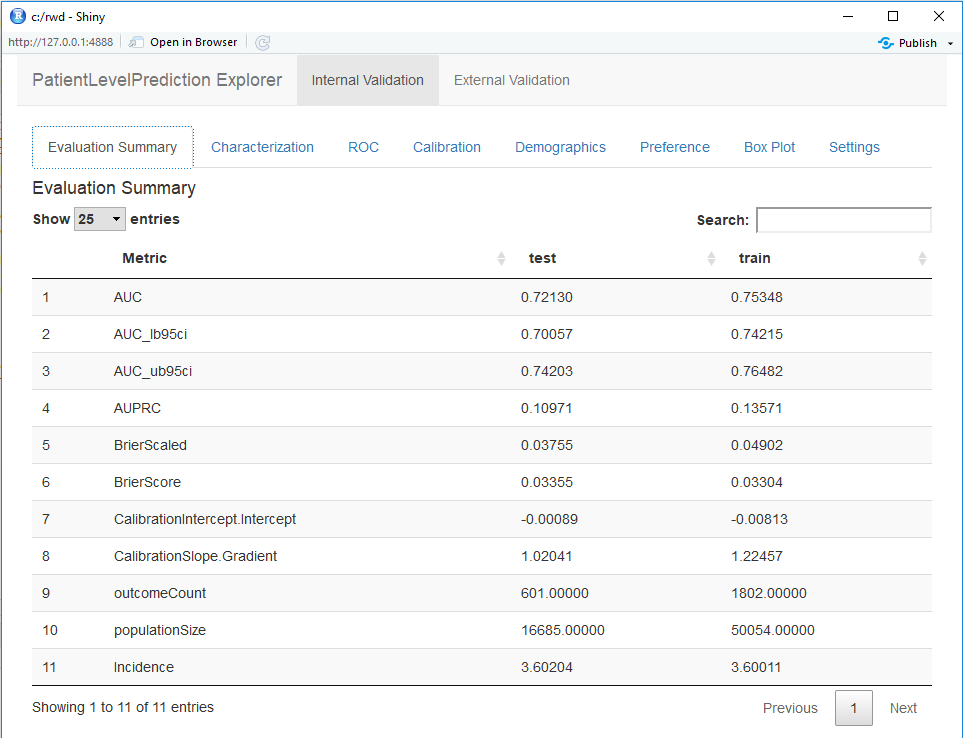
\includegraphics[width=1\linewidth]{images/PatientLevelPrediction/shinysummary}

To generate and save all the evaluation plots to a folder run the
following code:

\begin{Shaded}
\begin{Highlighting}[]
\KeywordTok{plotPlp}\NormalTok{(gbmResults, }\StringTok{"plots"}\NormalTok{)}
\end{Highlighting}
\end{Shaded}

The plots are described in more detail in the next sections.

\subsection{Discrimination}\label{discrimination}

The Receiver Operating Characteristics (ROC) plot shows the sensitivity
against 1-specificity on the test set. The plot illustrates how well the
model is able to discriminate between the people with the outcome and
those without. The dashed diagonal line is the performance of a model
that randomly assigns predictions. The higher the area under the ROC
plot the better the discrimination of the model. Figure \ref{fig:roc} is
created by changing the probability threshold to assign the positive
class.

\textbf{Todo: update plots with hypertension example}

\begin{figure}

{\centering 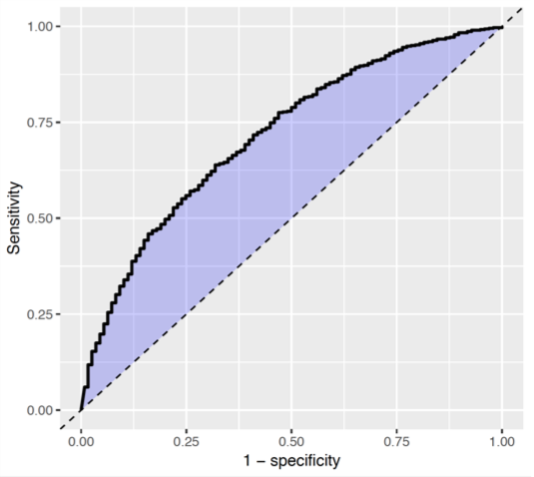
\includegraphics[width=0.8\linewidth]{images/PatientLevelPrediction/sparseROC} 

}

\caption{The Receiver Operating Characteristics (ROC) curve.}\label{fig:roc}
\end{figure}

\subsection{Calibration}\label{calibration}

The calibration plot (Figure \ref{fig:plpCalibration}) shows how close
the predicted risk is to the observed risk. The diagonal dashed line
thus indicates a perfectly calibrated model. The ten (or fewer) dots
represent the mean predicted values for each quantile plotted against
the observed fraction of people in that quantile who had the outcome
(observed fraction). The straight black line is the linear regression
using these 10 plotted quantile mean predicted vs observed fraction
points. The straight vertical lines represented the 95\% lower and upper
confidence intervals of the slope of the fitted line.

\begin{figure}

{\centering 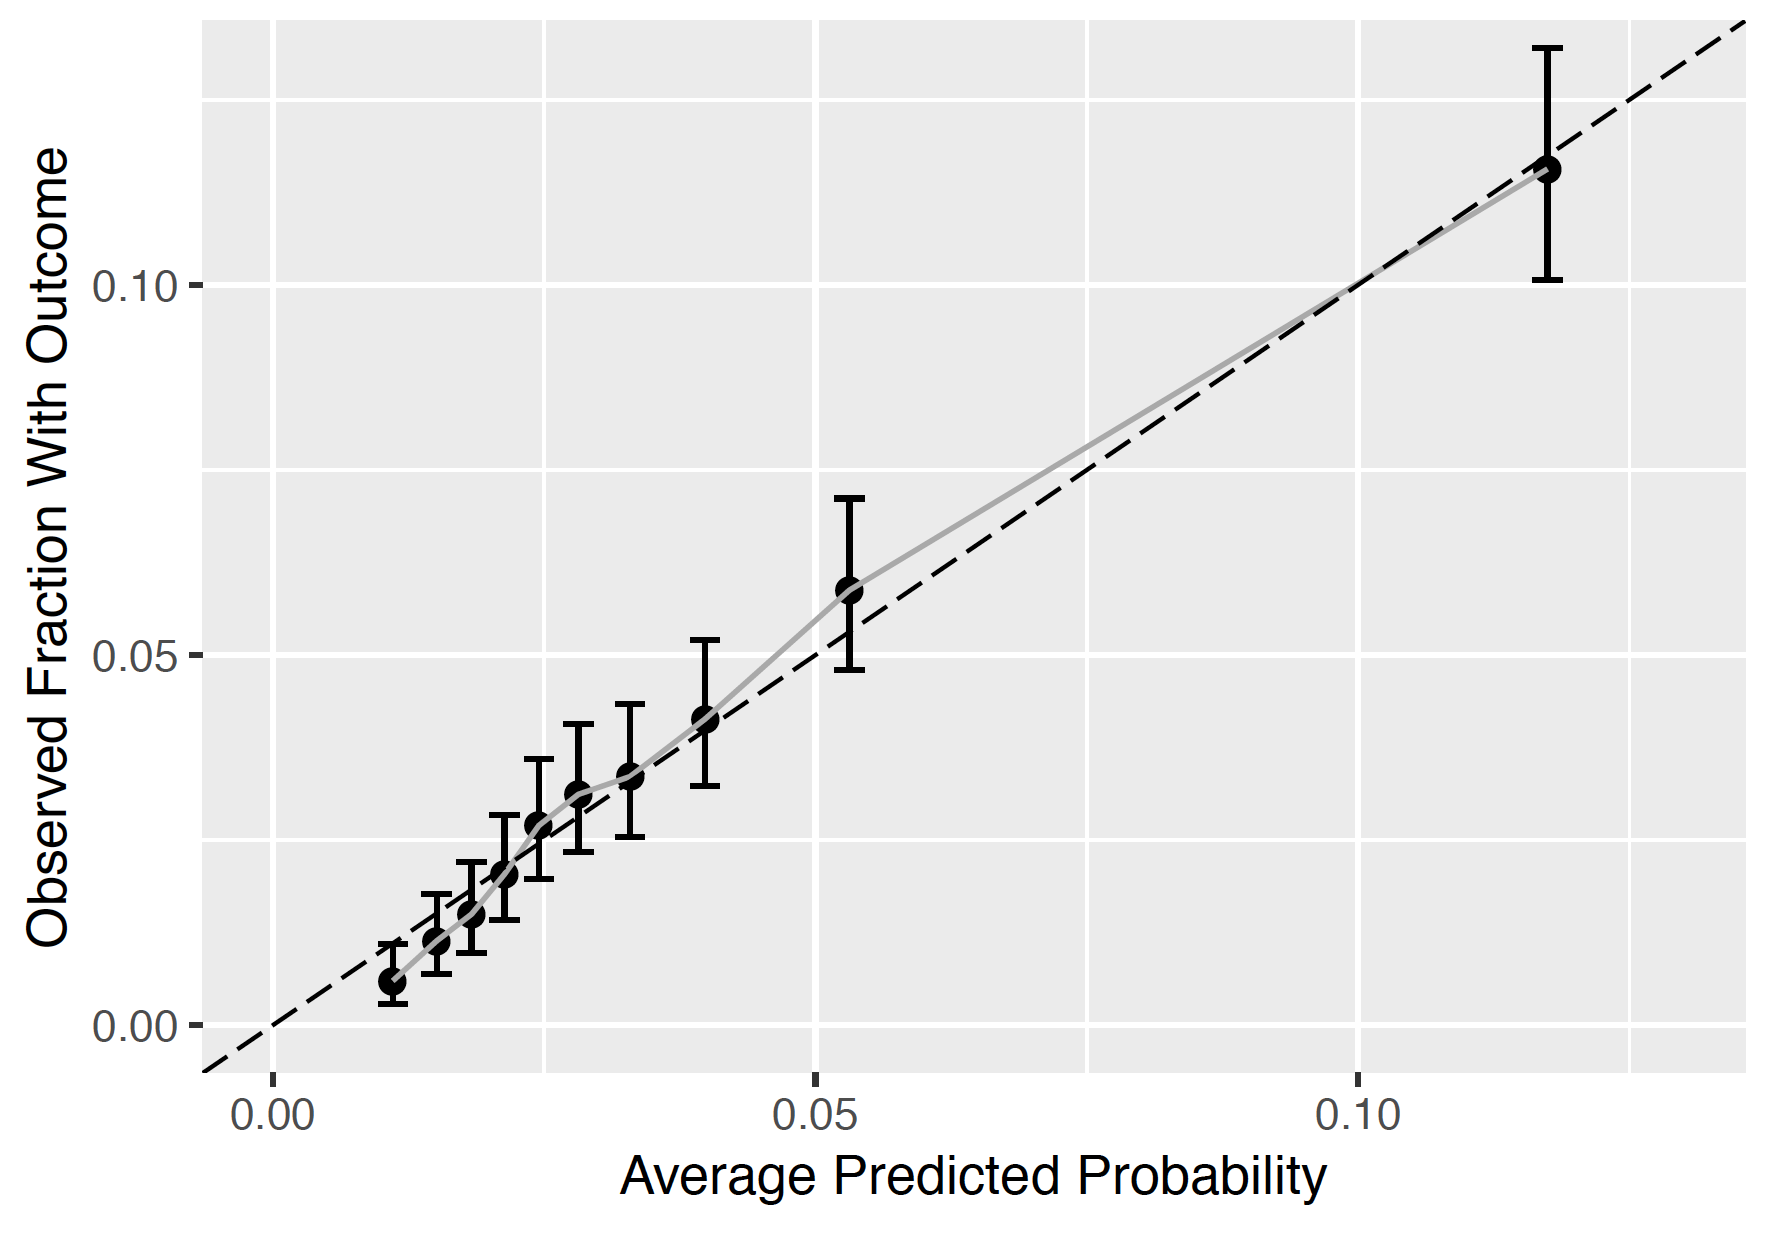
\includegraphics[width=0.9\linewidth]{images/PatientLevelPrediction/sparseCalibration} 

}

\caption{Calibration plot.}\label{fig:plpCalibration}
\end{figure}

\subsection{Smooth Calibration}\label{smooth-calibration}

Similar to the traditional calibration shown above the Smooth
Calibration plot shows the relationship between predicted and observed
risk. the major difference is that the smooth fit allows for a more fine
grained examination of this. Whereas the traditional plot will be
heavily influenced by the areas with the highest density of data the
smooth plot will provide the same information for this region as well as
a more accurate interpretation of areas with lower density. the plot
also contains information on the distribution of the outcomes relative
to predicted risk.

However, the increased information gain comes at a computational cost.
It is recommended to use the traditional plot for examination and then
to produce the smooth plot for final versions. To create the smooth
calibarion plot you have to run the follow command:

\begin{Shaded}
\begin{Highlighting}[]
\KeywordTok{plotSmoothCalibration}\NormalTok{(gbmResults)}
\end{Highlighting}
\end{Shaded}

See the help function for more information, on how to set the smoothing
method etc.

Figure \ref{fig:plpSmoothCal} shows an example from another study that
better demonstrates the impact of using a smooth calibration plot. The
default line fit would not highlight the miss-calibration at the lower
predicted probability levels that well.

\begin{figure}

{\centering 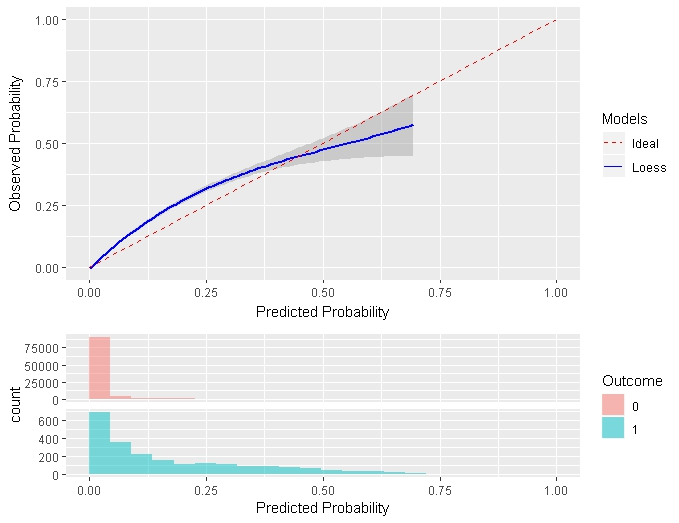
\includegraphics[width=1\linewidth]{images/PatientLevelPrediction/smoothCalibration} 

}

\caption{Smooth calibration plot.}\label{fig:plpSmoothCal}
\end{figure}

\subsection{Preference distribution}\label{preference-distribution}

The preference distribution plot (Figure \ref{fig:plpPreference}) shows
the preference score distributions for people in the test set with the
outcome (red) without the outcome (blue).

\begin{figure}

{\centering 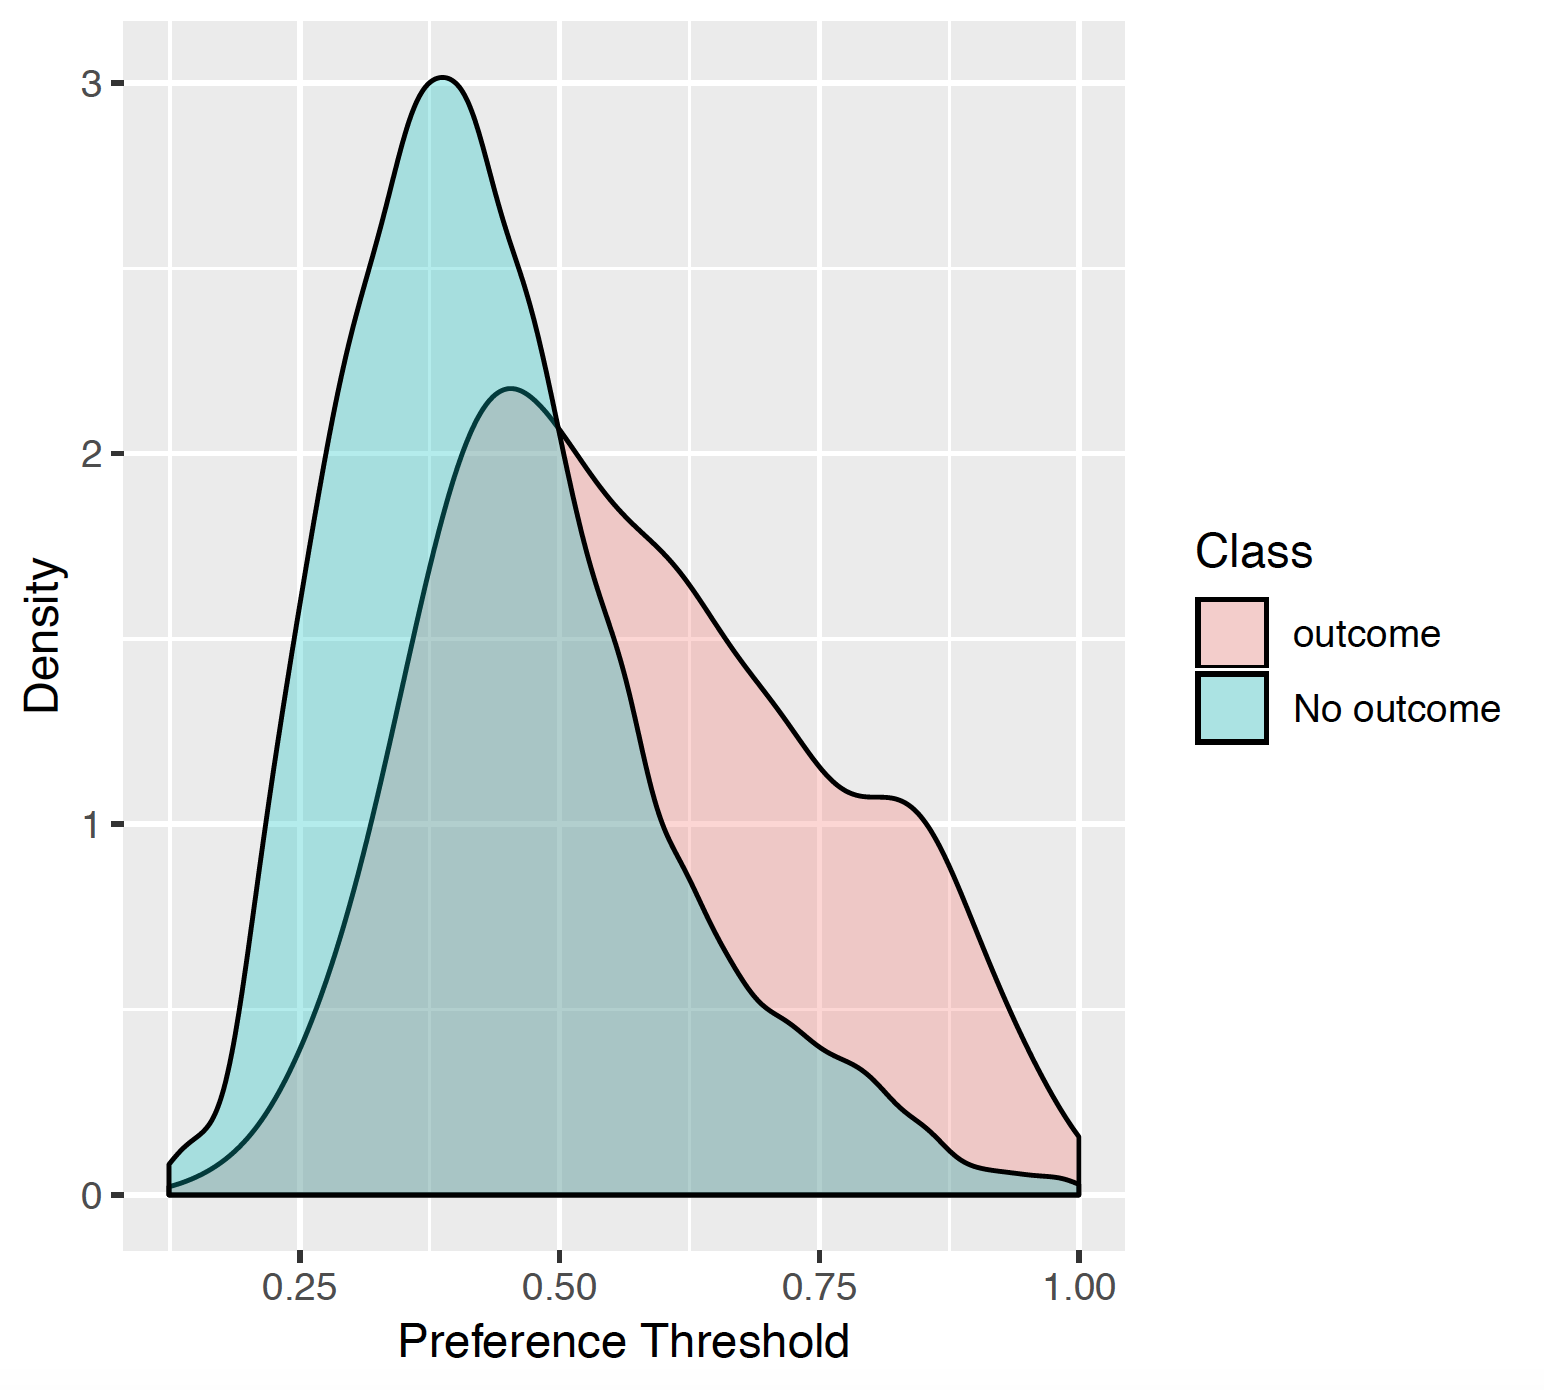
\includegraphics[width=0.9\linewidth]{images/PatientLevelPrediction/preferencePDF} 

}

\caption{Preference distribution plot.}\label{fig:plpPreference}
\end{figure}

\subsection{Predicted probability
distribution}\label{predicted-probability-distribution}

The prediction distribution box plot shows the predicted risks of the
people in the test set with the outcome (blue) and without the outcome
(red).

The box plots in Figure \ref{fig:plpPredProb} show that the predicted
probability of the outcome is indeed higher for those with the outcome
but there is also overlap between the two distribution which lead to an
imperfect discrimination.

\begin{figure}

{\centering 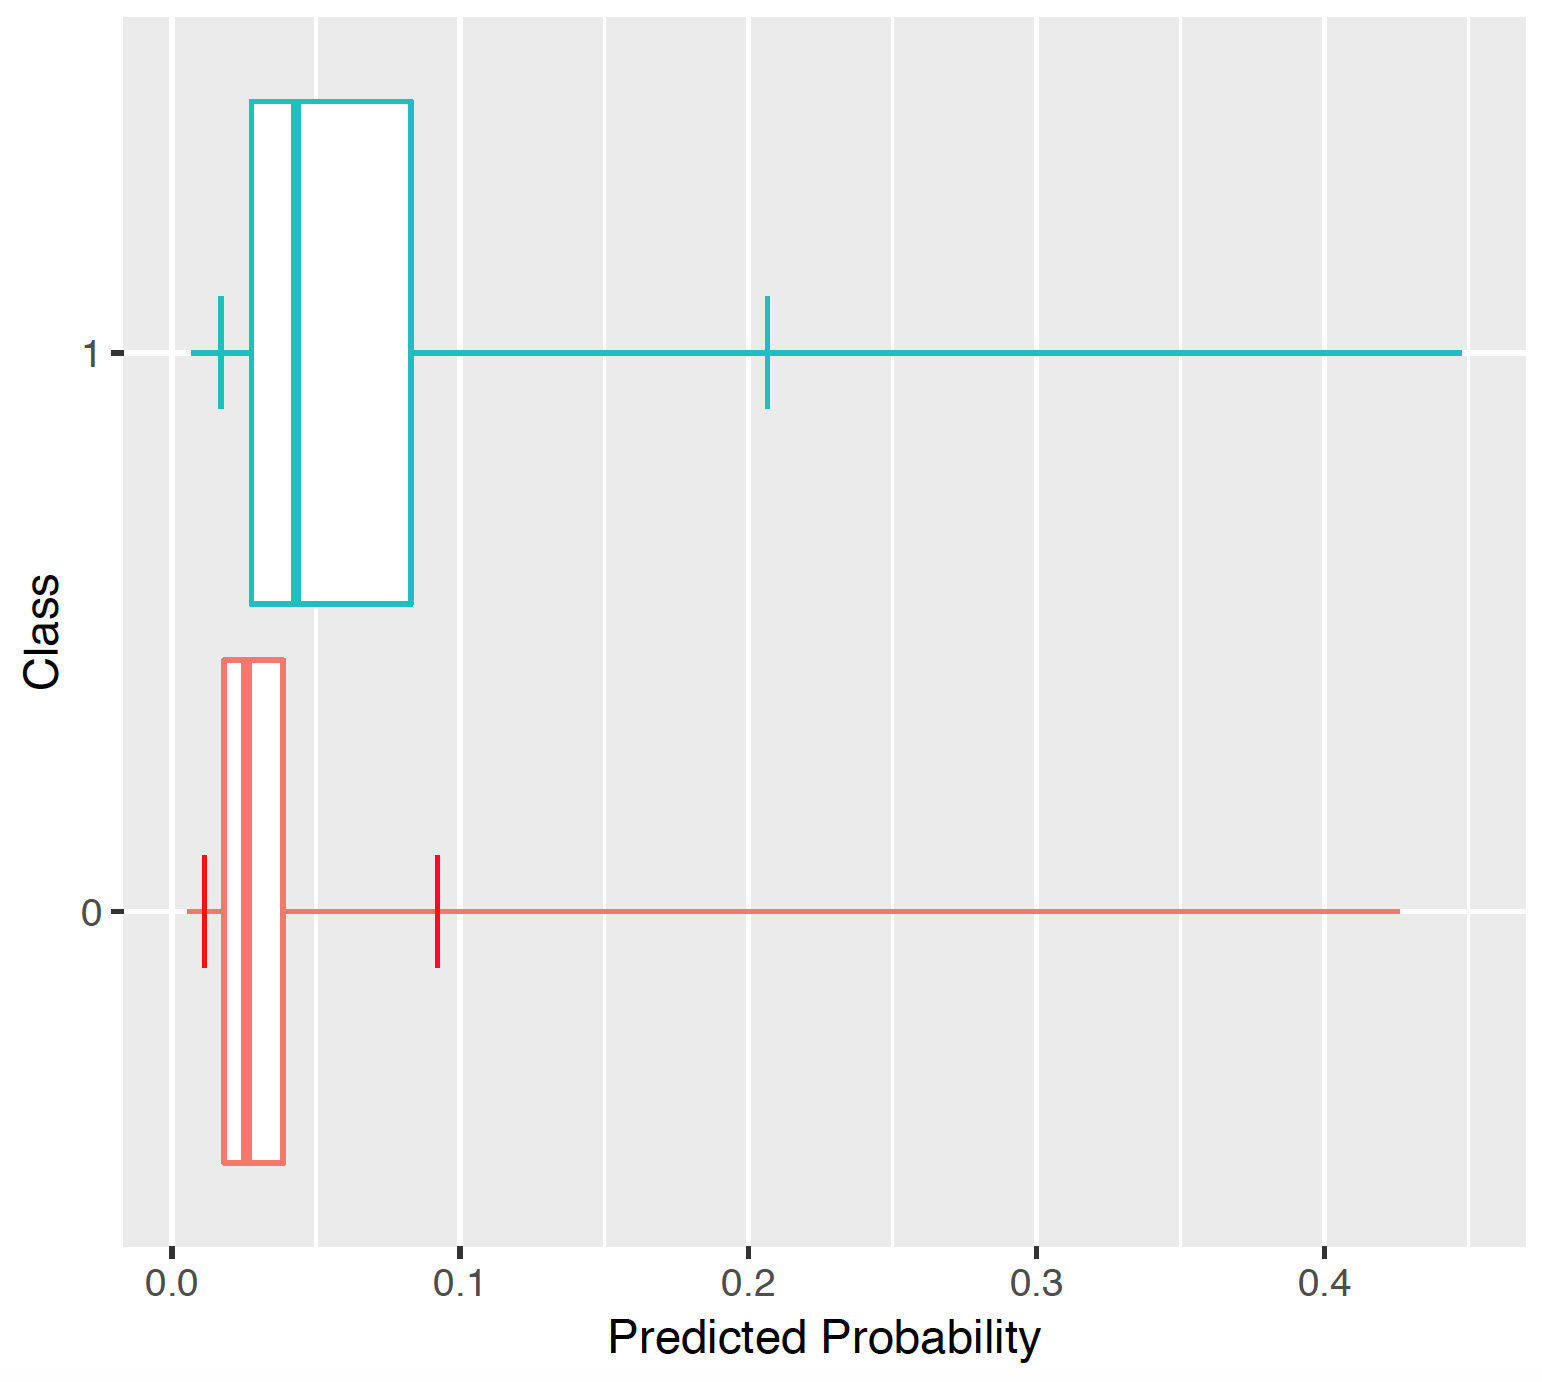
\includegraphics[width=0.9\linewidth]{images/PatientLevelPrediction/predictionDistribution} 

}

\caption{Predicted probability distribution.}\label{fig:plpPredProb}
\end{figure}

\subsection{Test-Train similarity}\label{test-train-similarity}

The test-train similarity is assessed by plotting the mean covariate
values in the train set against those in the test set for people with
and without the outcome.

The results in Figure \ref{fig:plpTestTrain} for our example look very
promising since the mean values of the covariates are on the diagonal.

\begin{figure}

{\centering 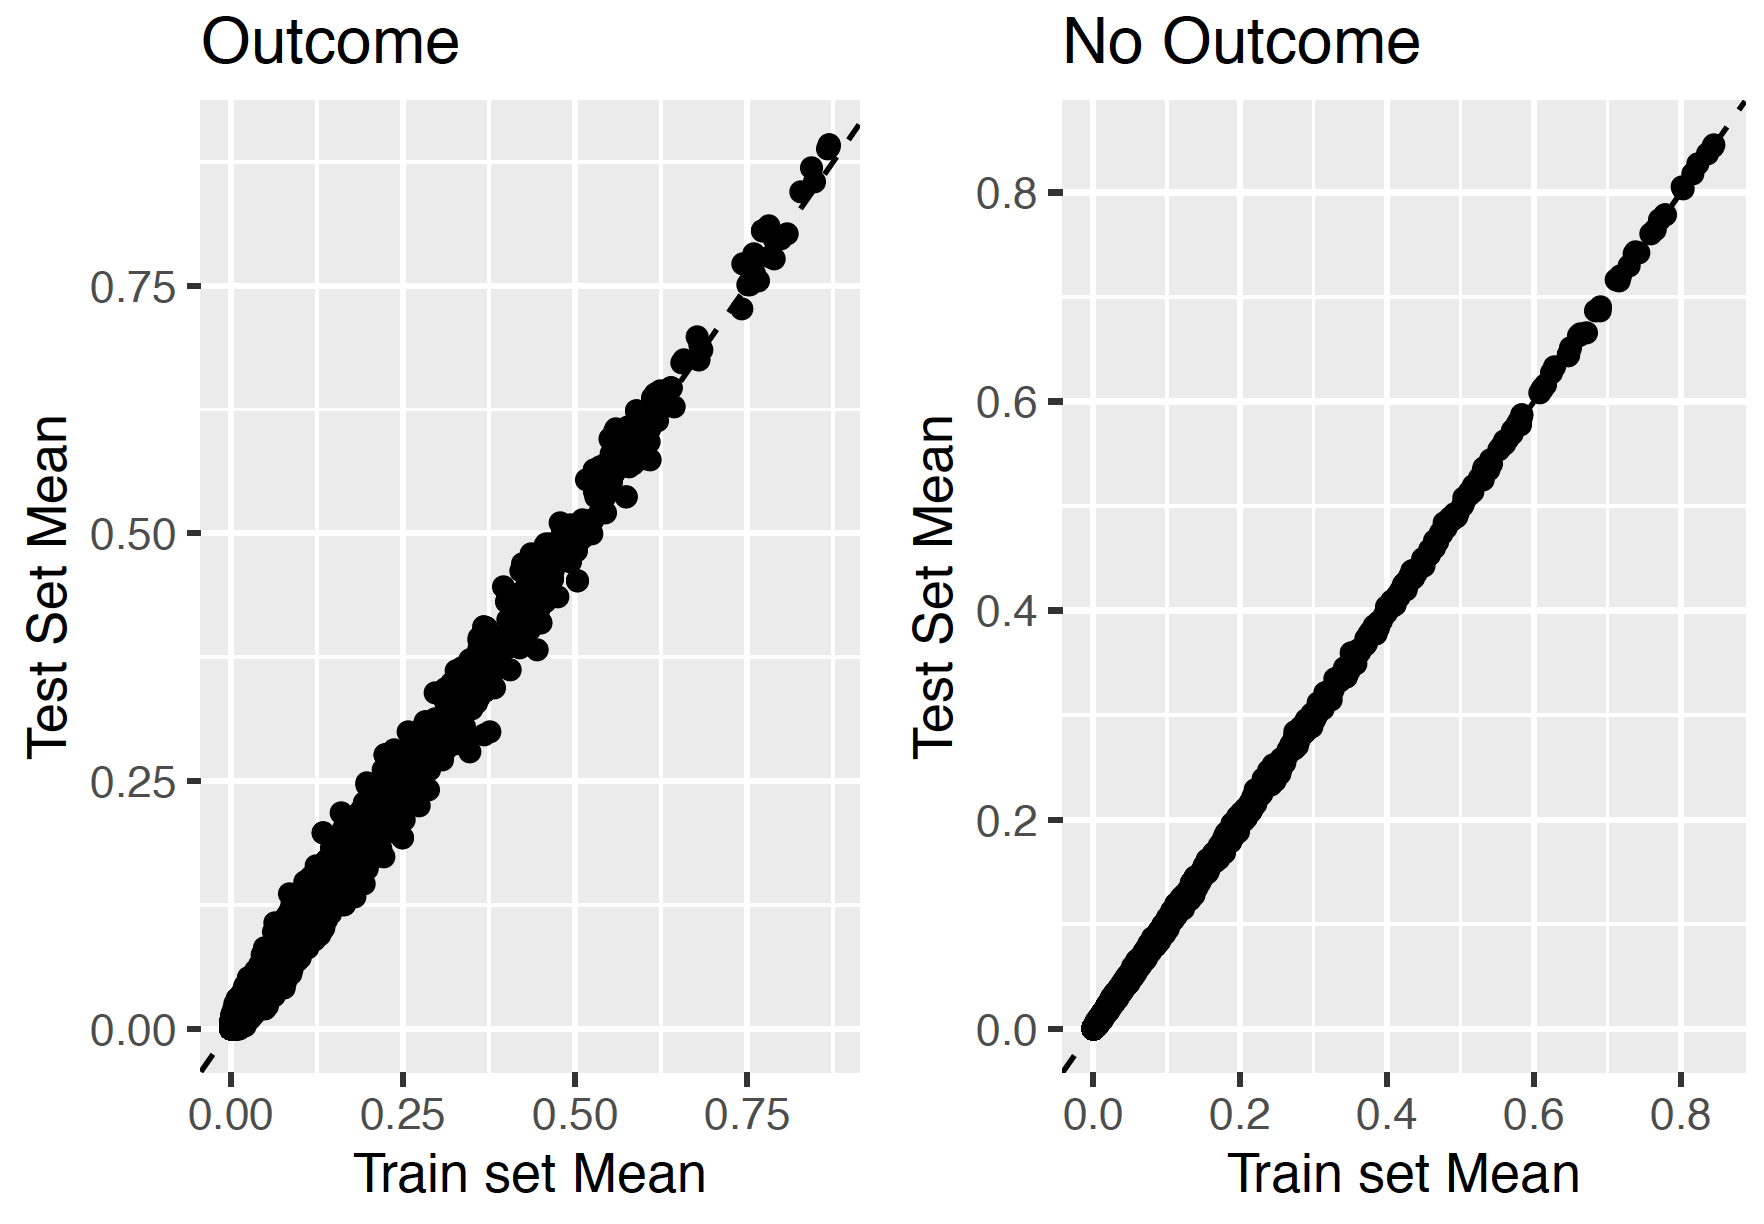
\includegraphics[width=1\linewidth]{images/PatientLevelPrediction/generalizability} 

}

\caption{Predicted probability distribution.}\label{fig:plpTestTrain}
\end{figure}

\subsection{Variable scatter plot}\label{variable-scatter-plot}

The variable scatter plot shows the mean covariate value for the people
with the outcome against the mean covariate value for the people without
the outcome. The color of the dots corresponds to the inclusion (green)
or exclusion in the model (blue), respectively. It is highly recommended
to use the Shiny App since this allows you to hoover over a covariate to
show more details (name, value etc).

Figure \ref{fig:plpVarScatter} shows that the mean of most of the
covariates is higher for subjects with the outcome compared to those
without.

\begin{figure}

{\centering 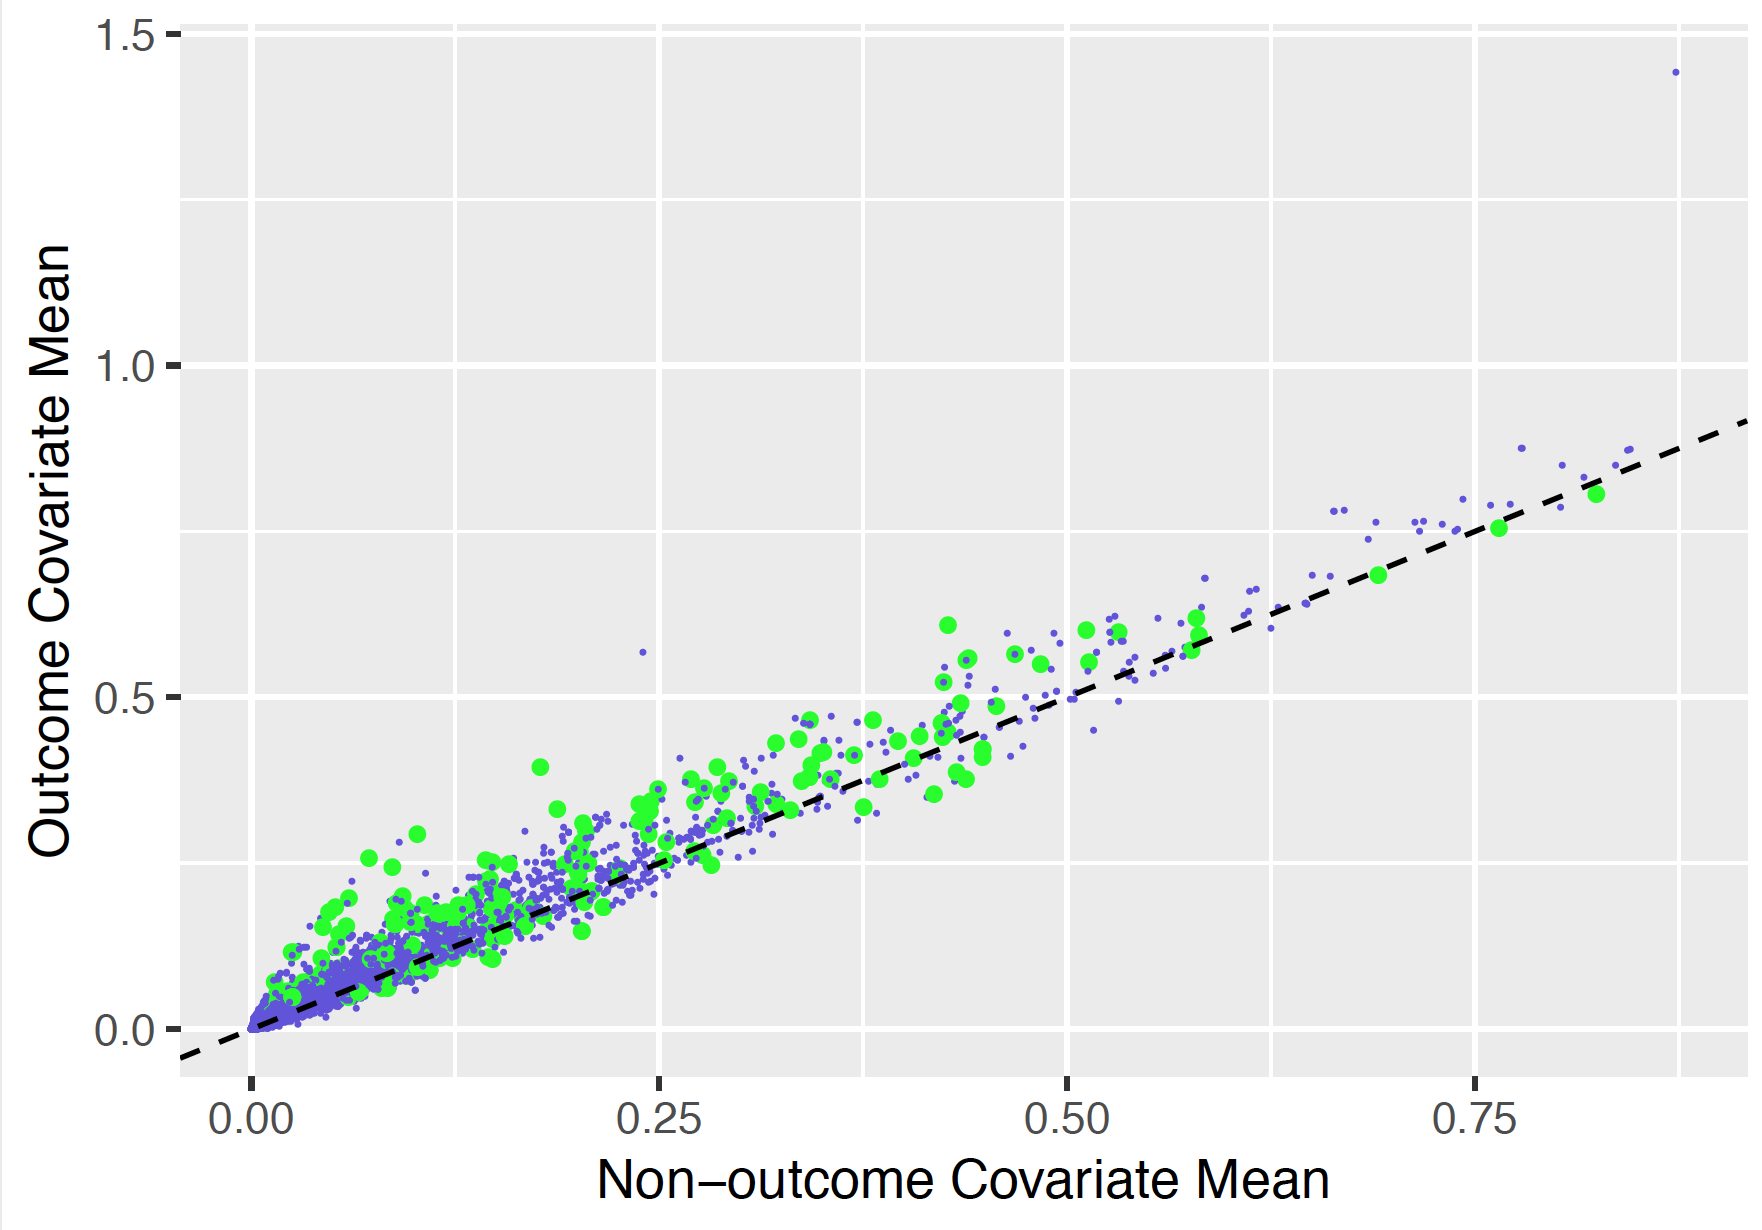
\includegraphics[width=1\linewidth]{images/PatientLevelPrediction/variableScatterplot} 

}

\caption{Predicted probability distribution.}\label{fig:plpVarScatter}
\end{figure}

\subsection{Precision recall}\label{precision-recall}

Precision (P) is defined as the number of true positives (TP) over the
number of true positives plus the number of false positives (FP):

\[P\ =\frac{\ TP}{TP\ +\ FP}\]

Recall (R) is defined as the number of true positives over the number of
true positives plus the number of false negatives (FN):

\[R\ =\frac{\ TP}{TP\ +\ FN}\]

These quantities are also related to the (F1) score, which is defined as
the harmonic mean of precision and recall.

\[F1\ =\ 2\ \cdot\ \frac{P\cdot R}{P+R}\]

Note that the precision can either decrease or increase if the threshold
is lowered. Lowering the threshold of a classifier may increase the
denominator, by increasing the number of results returned. If the
threshold was previously set too high, the new results may all be true
positives, which will increase precision. If the previous threshold was
about right or too low, further lowering the threshold will introduce
false positives, decreasing precision. For Recall the denominator does
not depend on the classifier threshold (Tp+Fn is a constant). This means
that lowering the classifier threshold may increase recall, by
increasing the number of true positive results. It is also possible that
lowering the threshold may leave recall unchanged, while the precision
fluctuates.

Figure \ref{fig:plpPrecisionRecall} shows the tradeoff between precision
and recall.

\begin{figure}

{\centering 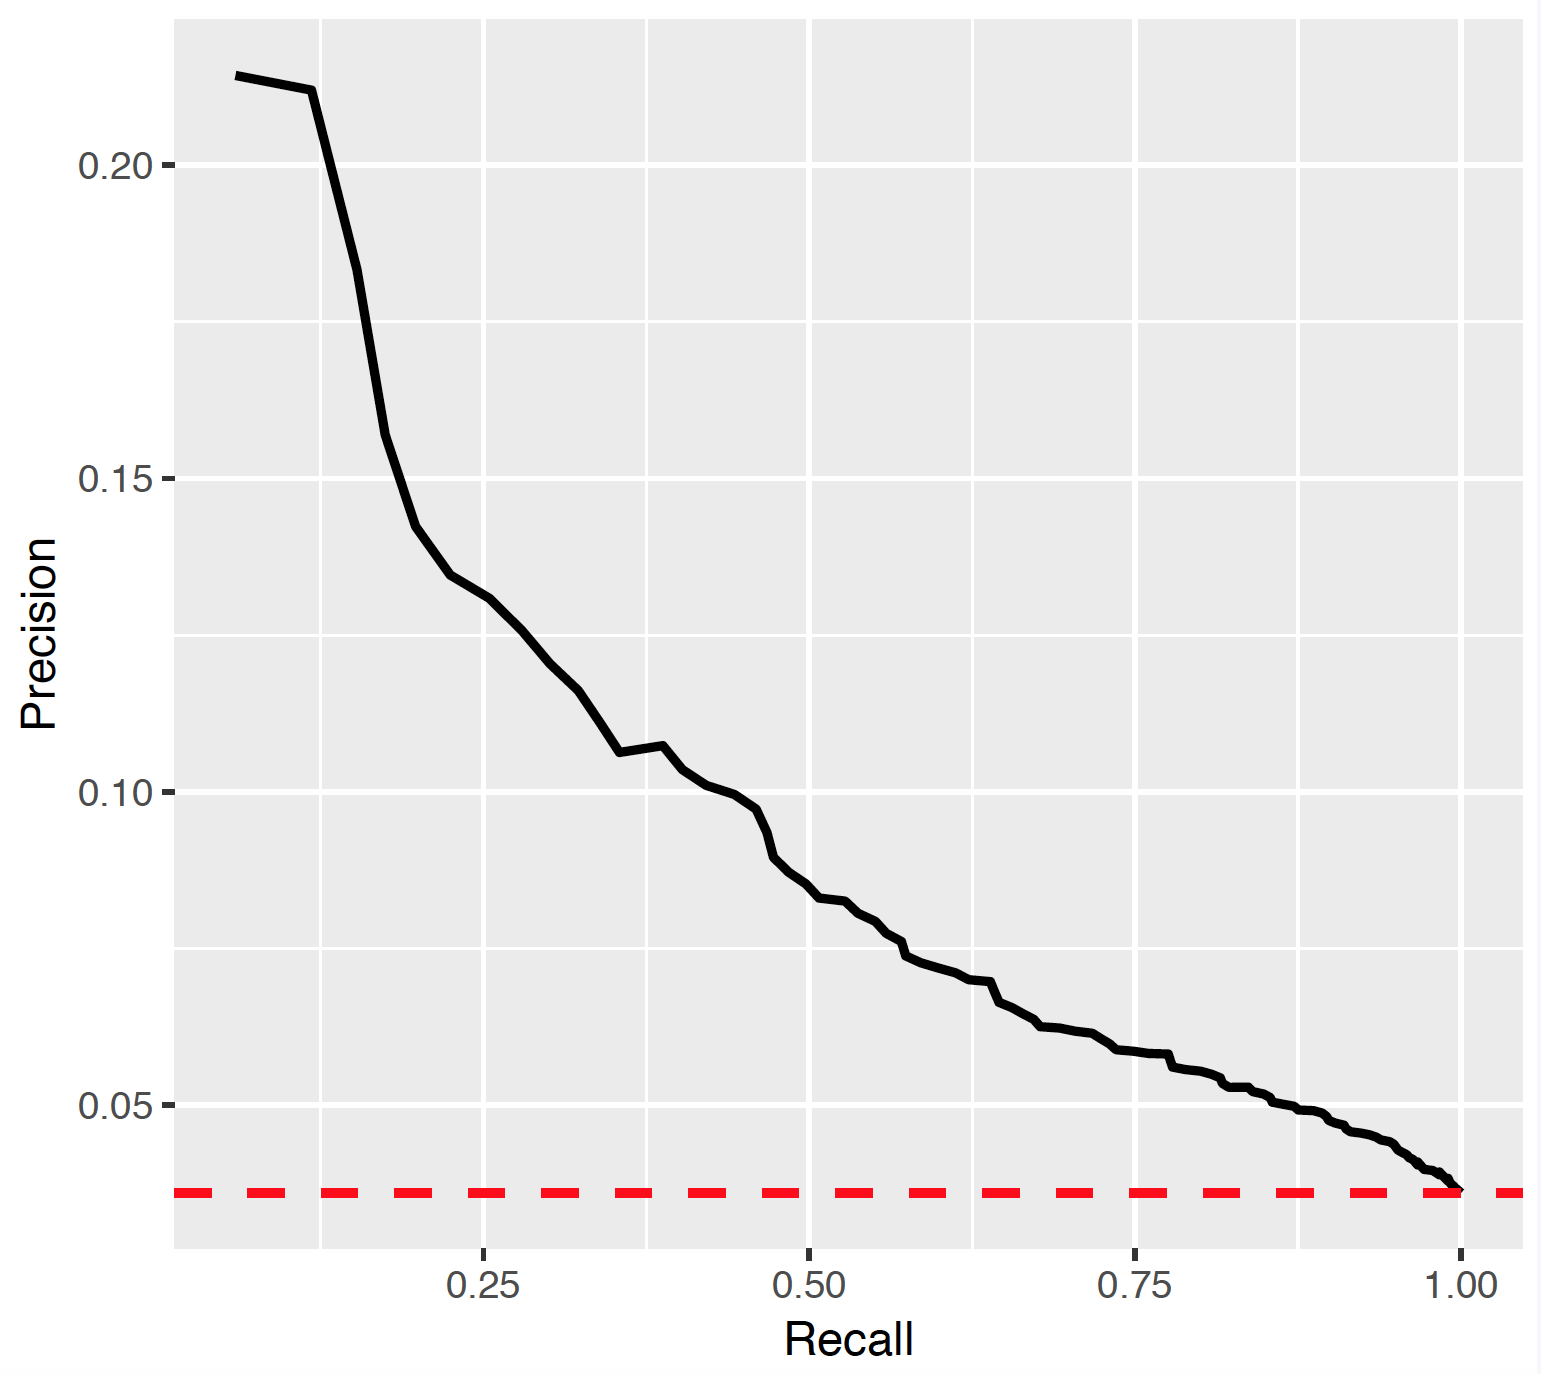
\includegraphics[width=0.8\linewidth]{images/PatientLevelPrediction/precisionRecall} 

}

\caption{Precision-recall plot.}\label{fig:plpPrecisionRecall}
\end{figure}

\subsection{Demographic summary}\label{demographic-summary}

Figure \ref{fig:plpDemoSummary} shows for females and males the expected
and observed risk in different age groups together with a confidence
area. The results show that our model is well calibrated across gender
and age groups.

\begin{figure}

{\centering 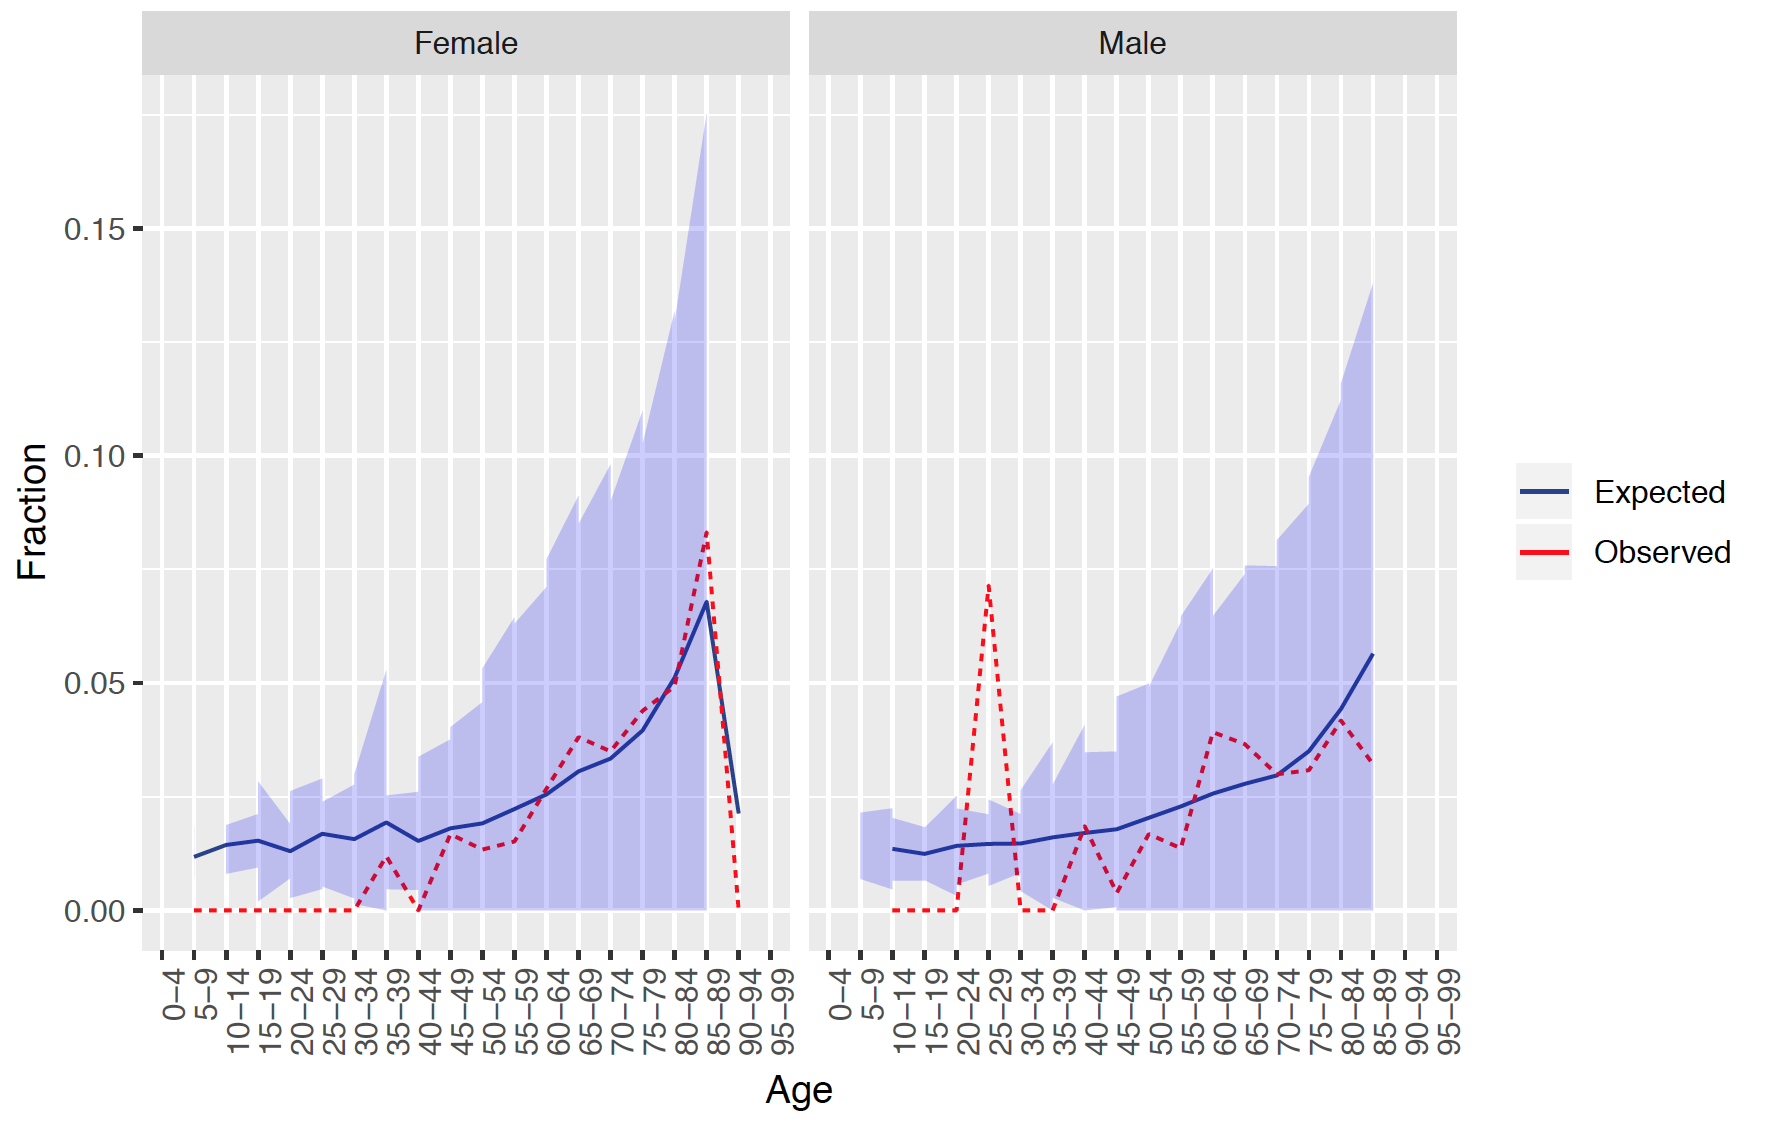
\includegraphics[width=1\linewidth]{images/PatientLevelPrediction/demographicSummary} 

}

\caption{Precision-recall plot.}\label{fig:plpDemoSummary}
\end{figure}

\section{External validation}\label{external-validation}

We recommend to always perform external validation, i.e.~apply the final
model on as much new datasets as feasible and evaluate its performance.
Here we assume the data extraction has already been peformed on a second
database and stored in the \texttt{newData} folder. We load the model we
previously fitted from the \texttt{model} folder:

\begin{Shaded}
\begin{Highlighting}[]
\CommentTok{# load the trained model}
\NormalTok{plpModel <-}\StringTok{ }\KeywordTok{loadPlpModel}\NormalTok{(}\StringTok{"model"}\NormalTok{)}

\CommentTok{#load the new plpData and create the population}
\NormalTok{plpData <-}\StringTok{ }\KeywordTok{loadPlpData}\NormalTok{(}\StringTok{"newData"}\NormalTok{)}

\NormalTok{population <-}\StringTok{ }\KeywordTok{createStudyPopulation}\NormalTok{(}\DataTypeTok{plpData =}\NormalTok{ plpData,}
                                    \DataTypeTok{outcomeId =} \DecValTok{2}\NormalTok{,}
                                    \DataTypeTok{washoutPeriod =} \DecValTok{364}\NormalTok{,}
                                    \DataTypeTok{firstExposureOnly =} \OtherTok{FALSE}\NormalTok{,}
                                    \DataTypeTok{removeSubjectsWithPriorOutcome =} \OtherTok{TRUE}\NormalTok{,}
                                    \DataTypeTok{priorOutcomeLookback =} \DecValTok{9999}\NormalTok{,}
                                    \DataTypeTok{riskWindowStart =} \DecValTok{1}\NormalTok{,}
                                    \DataTypeTok{riskWindowEnd =} \DecValTok{365}\NormalTok{,}
                                    \DataTypeTok{addExposureDaysToStart =} \OtherTok{FALSE}\NormalTok{,}
                                    \DataTypeTok{addExposureDaysToEnd =} \OtherTok{FALSE}\NormalTok{,}
                                    \DataTypeTok{minTimeAtRisk =} \DecValTok{364}\NormalTok{,}
                                    \DataTypeTok{requireTimeAtRisk =} \OtherTok{TRUE}\NormalTok{,}
                                    \DataTypeTok{includeAllOutcomes =} \OtherTok{TRUE}
\NormalTok{)}

\CommentTok{# apply the trained model on the new data}
\NormalTok{validationResults <-}\StringTok{ }\KeywordTok{applyModel}\NormalTok{(population, plpData, plpModel)}
\end{Highlighting}
\end{Shaded}

To make things easier we also provide the \texttt{externalValidatePlp}
function for performing external validation that also extracts the
required data. This function is described in the package manual.

\section{Journal paper generation}\label{journal-paper-generation}

We have added functionality to automatically generate a word document
you can use as start of a journal paper. It contains many of the
generated study details and results. If you have performed external
validation these results will can be added as well. Optionally, you can
add a ``Table 1'' that contains data on many covariates for the target
population. You can create the draft journal paper by running this
function:

\begin{Shaded}
\begin{Highlighting}[]
 \KeywordTok{createPlpJournalDocument}\NormalTok{(}\DataTypeTok{plpResult =} \OperatorTok{<}\NormalTok{your plp results}\OperatorTok{>}\NormalTok{,}
                          \DataTypeTok{plpValidation =} \OperatorTok{<}\NormalTok{your validation results}\OperatorTok{>}\NormalTok{,}
                          \DataTypeTok{plpData =} \OperatorTok{<}\NormalTok{your plp data}\OperatorTok{>}\NormalTok{,}
                          \DataTypeTok{targetName =} \StringTok{"<target population>"}\NormalTok{,}
                          \DataTypeTok{outcomeName =} \StringTok{"<outcome>"}\NormalTok{,}
                          \DataTypeTok{table1 =}\NormalTok{ F,}
                          \DataTypeTok{connectionDetails =} \OtherTok{NULL}\NormalTok{,}
                          \DataTypeTok{includeTrain =} \OtherTok{FALSE}\NormalTok{,}
                          \DataTypeTok{includeTest =} \OtherTok{TRUE}\NormalTok{,}
                          \DataTypeTok{includePredictionPicture =} \OtherTok{TRUE}\NormalTok{,}
                          \DataTypeTok{includeAttritionPlot =} \OtherTok{TRUE}\NormalTok{,}
                          \DataTypeTok{outputLocation =} \StringTok{"<your location>"}\NormalTok{)}
\end{Highlighting}
\end{Shaded}

For more details see the help page of the function.

\section{Excercises}\label{excercises-1}

\part{Evidence Quality}\label{part-evidence-quality}

\chapter{Evidence Quality}\label{EvidenceQuality}

\begin{quote}
Loss of fidelity begins with the movement of data from the doctor's
brain to the medical record.
\end{quote}

\emph{Clem McDonald, MD} \emph{Director, Lister Hill Center for
Biomedical Informatics} \emph{National Library of Medicine, USA}

OHDSI views validation as a holistic set of processes necessary to
achieve the highest quality reproducible evidence from diverse data
sources.

Four components: - Data quality (data validation) - Clinical validity -
Software validity - Method validity

\chapter{Data Quality}\label{DataQuality}

\section{Introduction}\label{introduction}

Kahn et al. define data quality as consisting of three components: (1)
conformance (do data values adhere to do specified standard and
formats?; subtypes: value, relational and computational conformance);
(2) completeness (are data values present?); and (3) plausibility (are
data values believable?; subtypes uniqueness, atemporal; temporal)
\citep{kahn_harmonized_2016}

Kahn additionaly defines two contexts: verification and validation.
Verification focuses on model and data constraints and does not rely on
external reference. Validation focuses on data expectations that are
derived from comparison to a relative gold standard and uses external
knowledge.

\begin{longtable}[]{@{}lll@{}}
\toprule
\begin{minipage}[b]{0.09\columnwidth}\raggedright\strut
Term\strut
\end{minipage} & \begin{minipage}[b]{0.16\columnwidth}\raggedright\strut
Subtype\strut
\end{minipage} & \begin{minipage}[b]{0.67\columnwidth}\raggedright\strut
Validation example\strut
\end{minipage}\tabularnewline
\midrule
\endhead
\begin{minipage}[t]{0.09\columnwidth}\raggedright\strut
Conformance\strut
\end{minipage} & \begin{minipage}[t]{0.16\columnwidth}\raggedright\strut
Value\strut
\end{minipage} & \begin{minipage}[t]{0.67\columnwidth}\raggedright\strut
Providers are only assigned valid medical specialties.\strut
\end{minipage}\tabularnewline
\begin{minipage}[t]{0.09\columnwidth}\raggedright\strut
\strut
\end{minipage} & \begin{minipage}[t]{0.16\columnwidth}\raggedright\strut
Relational\strut
\end{minipage} & \begin{minipage}[t]{0.67\columnwidth}\raggedright\strut
Prescribing provider identifier is present in drug dispensation
data.\strut
\end{minipage}\tabularnewline
\begin{minipage}[t]{0.09\columnwidth}\raggedright\strut
\strut
\end{minipage} & \begin{minipage}[t]{0.16\columnwidth}\raggedright\strut
Computational\strut
\end{minipage} & \begin{minipage}[t]{0.67\columnwidth}\raggedright\strut
Computed eGFR value conforms to the expected value for a test case
patient scenario.\strut
\end{minipage}\tabularnewline
\begin{minipage}[t]{0.09\columnwidth}\raggedright\strut
Completeness\strut
\end{minipage} & \begin{minipage}[t]{0.16\columnwidth}\raggedright\strut
n/a (no subtypes defined)\strut
\end{minipage} & \begin{minipage}[t]{0.67\columnwidth}\raggedright\strut
A drug product withdrawn from the market at a specific absolute historic
date shows expected drop in dispensation.\strut
\end{minipage}\tabularnewline
\begin{minipage}[t]{0.09\columnwidth}\raggedright\strut
Plausibility\strut
\end{minipage} & \begin{minipage}[t]{0.16\columnwidth}\raggedright\strut
Uniqueness\strut
\end{minipage} & \begin{minipage}[t]{0.67\columnwidth}\raggedright\strut
A zip code for a location does not refer to vastly conflicting
geographical areas.\strut
\end{minipage}\tabularnewline
\begin{minipage}[t]{0.09\columnwidth}\raggedright\strut
\strut
\end{minipage} & \begin{minipage}[t]{0.16\columnwidth}\raggedright\strut
Atemporal\strut
\end{minipage} & \begin{minipage}[t]{0.67\columnwidth}\raggedright\strut
Use of a medication (by age group) for a specific disease agrees with
the age pattern for that disease.\strut
\end{minipage}\tabularnewline
\begin{minipage}[t]{0.09\columnwidth}\raggedright\strut
\strut
\end{minipage} & \begin{minipage}[t]{0.16\columnwidth}\raggedright\strut
Temporal\strut
\end{minipage} & \begin{minipage}[t]{0.67\columnwidth}\raggedright\strut
Temporal pattern of an outbreak of a disease (e.g., Zika) agrees with
external source pattern.\strut
\end{minipage}\tabularnewline
\bottomrule
\end{longtable}

Kahn introduces the term \emph{data quality check} (sometimes refered to
as data quality rule) that tests whether data conform to a given
requirement (e.g., implausible age of 141 of a patient (due to incorrect
birth year or missing death event)). In support of checks, he also
defines \emph{data quality measure} (sometimes refered to as
pre-computed analysis) as data analysis that supports evaluation of a
check. For example, distribution of days of supply by drug concept.

Two types of DQ checks can be distinguished\citep{weiskopf_methods_2013}

\begin{itemize}
\tightlist
\item
  general checks
\item
  study-specific checks
\end{itemize}

From the point of researcher analyzing the data, the desired situation
is that data is free from erros that could have been prevented.
\emph{ETL data errors} are errors introduced during
extract-tranform-load proces. A special type of ETL data error is
\emph{mapping error} that results from incorrect mapping of the data
from the source terminology (e.g., Korean national drug terminology)
into the target data model's standard terminology (e.g., RxNorm and
RxNorm Extension). A \emph{source data error} is an error that is
already present in the source data due to various cuases (e.g., human
typo during data entry).

Data quality can also be seen as a component in a larger effort refered
to as \emph{evidence quality} or \emph{evidence validation}. Data
quality would fall in this framework under \emph{data validation}.

\section{Achilles Heel tool}\label{achilles-heel-tool}

Since 2014, a component of the OHDSI Achilles tool called Heel was used
to check data quality.\citep{huser_methods_2018}

\subsection{Precomputed Analyses}\label{precomputed-analyses}

In support of data characterization, Achilles tool pre-computes number
of data analyses. Each pre-computed analysis has an analysis ID and a
short description of the analysis. For example, ``715: Distribution of
days\_supply by drug\_concept\_id'' or ``506: Distribution of age at
death by gender''. List of all pre-computed analyses (for Achilles
version 1.6.3) as available at
\url{https://github.com/OHDSI/Achilles/blob/v1.6.3/inst/csv/achilles/achilles_analysis_details.csv}

Achilles has more than 170 pre-computed analysis that support not only
data quality checks but also general data characterization (outside data
quality context) such as data density visualizations. The
pre-computations are largely guided by the CDM relational database
schema and analyze most terminology-based data columns, such as
condition\_concept\_id or place\_of\_service\_concept\_id.
Pre-computations results are stored in table ACHILLES\_RESULTS and
ACHILLES\_RESULTS\_DIST.

\subsection{Example DQ check}\label{example-dq-check}

In complete data about general population, a range of services is
provided by a range of providers (with many specialties). A data
completness rule with rule\_id of 38 evaluates data completness in the
PROVIDER table. Checking optional fields in CDM (such as provider
specialty) lead to a notification severity output. Analysis Rule 38
triggers a notification if count of distinct specialties \textless{}2.
It relies on a derived measure \texttt{Provider:SpeciatlyCnt}. The rule
SQL-formulated logic can be found here:
\url{https://github.com/OHDSI/Achilles/blob/v1.6.3/inst/sql/sql_server/heels/serial/rule_38.sql}

\subsection{Overview of existing DQ Heel
checks}\label{overview-of-existing-dq-heel-checks}

Achilles developers maintain a list of all DQ checks in an overview
file. For version 1.6.3, this overview is available here
\url{https://github.com/OHDSI/Achilles/blob/v1.6.3/inst/csv/heel/heel_rules_all.csv}
Each DQ check has a rule\_id.

Checks are classified into CDM conformance checks and DQ checks.

Depending on the severity of the problem, the Heel output can be error,
warning or notification.

\section{Study-specific checks}\label{study-specific-checks}

The chapter has so far focused on general DQ checks. Such checks are
executed regardless of the single research question context. The
assumption is that a researcher would formulate additional DQ checks
that are required for a specific research question.

We use case studies to demostrate study-specific checks.

\subsection{Outcomes}\label{outcomes}

For an international analysis, part of OHDSI study diagnostics (for a
give dataset) may involve checking whether coding practices (that are
country specific) affect a cohort definition. A stringent cohort
definition may lead to zero cohort size in one (or multiple dataesets).

\subsection{Laboratory data}\label{laboratory-data}

A diabetes study may utilize HbA1c measurement. A 2018 OHDSI study
(\url{https://www.ncbi.nlm.nih.gov/pubmed/30646124}) defined a cohort
`HbA1c8Moderate' (see
\url{https://github.com/rohit43/DiabetesTxPath/blob/master/inst/settings/CohortsToCreate.csv})

\chapter{Clinical Validity}\label{ClinicalValidity}

\chapter{Software Validity}\label{SoftwareValidity}

\emph{Chapter lead: Martijn Schuemie}

The central question of sofware validity is

\begin{quote}
Does the software do what it is expected to do?
\end{quote}

In broad strokes there are two approaches to ensure software validity:
by using a software development process aimed at creating valid
software, and by testing whether the software is valid. Here we focus
specifically on the \href{https://ohdsi.github.io/MethodsLibrary/}{OHDSI
Methods Library}, the set of R packages used in population-level
estimation and patient-level prediction. The OHDSI Population-Level
Estimation Workgroup and the OHDSI Patient-Level Prediction Workgroup
together are responsible for developing and maintaining the OHDSI
Methods Library. The OHDSI Population-Level Estimation Workgroup is
headed by Drs. Marc Suchard and Martijn Schuemie. The OHDSI
Patient-Level Prediction Workgroup his headed by Drs. Peter Rijnbeek and
Jenna Reps.

\section{Software Development
Process}\label{software-development-process}

The OHDSI Methods Library is developed by the OHDSI community. Proposed
changes to the Library are discussed in two venues: The GitHub issue
trackers and the \href{http://forums.ohdsi.org/}{OHDSI Forums}. Both are
open to the public. Any member of the community can contribute software
code to the Library, however, final approval of any changes incorporated
in the released versions of the software is performed by the OHDSI
Population-Level Estimation Workgroup and OHDSI Patient-Level Prediction
Workgroup leadership only.

Users can install the Methods Library in R directly from the master
branches in the GitHub repositories, or through a system known as `drat'
that is always up-to-date with the master branches. A number of the
Methods Library packages are available through R's Comprehensive R
Archive Network (CRAN), and this number is expected to increase over
time.

Reasonable software development and testing methodologies are employed
by OHDSI to maximize the accuracy, reliability and consistency of the
Methods Library performance. Importantly, as the Methods Library is
released under the terms of the Apache License V2, all source code
underlying the Methods Library, whether it be in R, C++, SQL, or Java is
available for peer review by all members of the OHDSI community, and the
public in general. Thus, all the functionality embodied within Methods
Library is subject to continuous critique and improvement relative to
its accuracy, reliability and consistency.

\subsection{Source Code Management}\label{source-code-management}

All of the Methods Library's source code is managed in the source code
version control system `git' publicly assessible via GitHub. The OHDSI
Methods Library repositories are access controlled. Anyone in the world
can view the source code, and any member of the OHDSI community can
submit changes through so-called pull requests. Only the OHDSI
Population-Level Estimation Workgroup and Patient-Level Prediction
Workgroup leadership can approve such request, make changes to the
master branches, and release new versions. Continuous logs of code
changes are maintained within the GitHub repositories and reflect all
aspects of changes in code and documentation. These commit logs are
available for public review.

New versions are released by the OHDSI Population-Level Estimation
Workgroup and Patient-Level Prediction Workgroup leadership as needed. A
new release starts by pushing changes to a master branch with a package
version number (as defined in the DESCRIPTION file inside the package)
that is greater than the version number of the previous release. This
automatically triggers checking and testing of the package. If all tests
are passed, the new version is automatically tagged in the version
control system and the package is automatically uploaded to the OHDSI
drat repository. New versions are numbered using three-component version
number:

\begin{itemize}
\tightlist
\item
  New micro versions (e.g.~from 4.3.2 to 4.3.3) indicate bug fixes only.
  No new functionality, and forward and backward compatibility are
  guaranteed
\item
  New minor versions (e.g.~from 4.3.3 to 4.4.0) indicate added
  functionality. Only backward compatibility is guaranteed
\item
  New major versions (e.g.~from 4.4.0 to 5.0.0) indicate major
  revisions. No guarantees are madef in terms of compatibility
\end{itemize}

\subsection{Documentation}\label{documentation}

All packages in the Methods Library are documented through R's internal
documentation framework. Each package has a package manual that
describes every function available in the package. To promote alignment
between the function documentation and the function implementation, the
roxygen2 software is used to combine a function's documentation and
source code in a single file. The package manual is available on demand
through R's command line interface, as a PDF in the package
repositories, and as a web page. In addition, many packages also have
vignettes that highlight specific use cases of a package. All Method
Library source code is available to end users. Feedback from the
community is facilitated using GitHub's issue tracking system and the
\href{http://forums.ohdsi.org/}{OHDSI Forums}.

\subsection{Availability of Current and Historical Archive
Versions}\label{availability-of-current-and-historical-archive-versions}

Current and historical versions of the Methods Library packages are
available in two locations: First, the GitHub version control system
contains the full development history of each package, and the state of
a package at each point in time can be reconstructed and retrieved. Most
importantly, each released version is tagged in GitHub. Second, the
released R source packages are stored in the OHDSI GitHub drat
repository.

\subsection{Maintenance, Support and
Retirement}\label{maintenance-support-and-retirement}

Each current version of the Methods Library is actively supported by
OHDSI with respect to bug reporting, fixes and patches. Issues can be
reported through GitHub's issue tracking system, and through the OHDSI
forums. Each package has a package manual, and zero, one or several
vignettes. Online video tutorials are available, and in-person tutorials
are provided from time to time.

\subsection{Qualified Personnel}\label{qualified-personnel}

Members of OHDSI community represent multiple statistical disciplines
and are based at academic, not-for-profit and industry-affiliated
institutions on multiple continents.

All leaders of the OHDSI Population-Level Estimation Workgroup and OHDSI
Patient-Level Prediction Workgroup hold PhDs from accredited academic
institutions and have published extensively in peer reviewed journals.

\subsection{Physical and Logical
Security}\label{physical-and-logical-security}

The OHDSI Methods Library is hosted on the
\href{https://github.com/}{GitHub} system. GitHub's security measures
are described at \url{https://github.com/security}. Usernames and
passwords are required by all members of the OHDSI community contribute
modifications to the Methods Library, and only the Population-Level
Estimation Workgroup and Patient-Level Prediction Workgroup leadership
can makes changes to the master branches. User accounts are limited in
access based upon standard security policies and functional
requirements.

\subsection{Disaster Recovery}\label{disaster-recovery}

The OHDSI Methods Library is hosted on the GitHub system. GitHub's
disaster recovery facilities are described at
\url{https://github.com/security}.

\section{Testing}\label{testing}

We distinguish between two types of tests performed on the Methods
Library: Tests for individual functions in the packages (so-called `unit
tests'), and tests to determine whether analyses implemented using the
Methods Library produce reliable and accurate results (we will call this
`method tests').

\subsection{Unit test}\label{unit-test}

A large set of automated validation tests is maintained and upgraded by
OHDSI to enable the testing of source code against known data and known
results. Each test begins with specifying some simple input data, then
executes a function in one of the packages on this input, and evaluates
whether the output is exactly what would be expected. For simple
functions, the expected result is often obvious (for example when
performing propensity score matching on example data containing only a
few subjects), for more complicated functions the expected result may be
generated using combinations of other functions available in R (for
example, Cyclops, our large-scale regression engine, is tested amongst
others by comparing results on simple problems with other regression
routines in R). We aim for these tests in total to cover 100\% of the
lines of executable source code. Appendix A lists the locations of the
tests in each package. These tests are automatically performed when
changes are made to a package (specifically, when changes are pushed to
the package repository). Any errors noted during testing automatically
trigger emails to the leadership of the Workgroups, and must be resolved
prior to release of a new version of a package. The results of the unit
tests can be found in the locations specified in Appendix A. The source
code and expected results for these tests are available for review and
use in other applications as may be appropriate. These tests are also
available to end users and/or system administrators and can be run as
part of their installation process to provide further documentation and
objective evidence as to the accuracy, reliability and consistency of
their installation of the Methods Library.

\section{Conclusions}\label{conclusions}

The purpose of this chapter is to document evidence to provide a high
degree of assurance that the Methods Library can be used in
observational studies to consistently produce reliable and accurate
estimates. Both through adoption of best software development practices
during the software lifecycle, as well as continuous extensive testing
of individual components of the software and the start-to-finish
application of the methods library on a gold standard aim to ensure the
validity of the Methods Library. However, use of the Methods Library
does not guarantee validity of a study, since validity depends on many
other components outside of the Methods Library as well, including
appropriate study design, exposure and outcome definitions, and data
quality. It is important to note that there is a significant obligation
on the part of the end-user's organization to define, create, implement
and enforce the Method Library installation, validation and utilization
related Standard Operating Procedures (SOPs) within the end-user's
environment. These SOPs should define appropriate and reasonable quality
control processes to manage end-user related risk within the applicable
operating framework. The details and content of any such SOPs are beyond
the scope of this document.

\chapter{Method Validity}\label{MethodValidity}

\emph{Chapter lead: Martijn Schuemie}

When considering method validity we aim to answer the question

\begin{quote}
Is this method valid for answering this question?
\end{quote}

Where `method' includes not only the study design, but als the data and
the implementation of the design. Method validity is therefore somewhat
of a catch-all; It is often not possible to observe good method validity
without good data quality, clinical validity, and software validity.
Those aspects of evidence quality should have already been addressed
separately before we consider method validity.

The core activity when establishing method validity is evaluating
whether important assumptions in the analysis have been met. For
example, we assume that propensity-score matching makes two populations
comparable, but we need to evaluate whether this is the case. Where
possible, empirical tests should be performed to test these assumptions.
We can for example generate diagnostics to show that our two populations
are indeed comparable on a wide range of characteristics after matching.
In OHDSI we have developed a wide range of standardized diagnostics that
should be generated and evaluated whenever an analysis is performed.
Some of these diagnostics are specific to certain stud designs, whereas
others are more generic.

\section{Design-specific diagnostics}\label{design-specific-diagnostics}

For each study design there are diagnostics specific to such a design.
Here we review some of the standard diagnostics included in the OHDSI
Methods Library R packages. This review is not exhaustive, and we
recommend the reader to consult the documentation for each method to
learn about all implemented diagnostics.

\subsection{Diagnostics for cohort
method}\label{diagnostics-for-cohort-method}

In the comparative cohort design we compare two cohorts, for example
representing two treatment choices, and we want to evaluate whether the
treatment choice has an effect on the risk of some outcome of interest.
For the effect size estimate w to be valid, it is essential that the two
groups are comparable in all relevant aspects except the treatment
choice. In observational data, this comparability is by no means
guaranteed, and quite often there is a reason why one group gets a
treatment while the group does not, leading to fundamental differences
between the groups. We often employ propensity scores to make the two
groups comparable again, but that assumes there is at least some
commonality between the two groups. This assumption can be tested by
reviewing the preference score plot as shown in Figure \ref{fig:ps} (The
preference score is a transformation of the propensity score that
adjusts for differences in the sizes of the two treatment groups). we
can evaluate whether there are patients that had some probability of
receiving either treatment. In Figure \ref{fig:ps} we see large numbers
of people on the left and right for whom their treatment choice could
have been predicted fairly accurately based on the baseline
characteristics, meaning that without adjustment the two groups are
incomparable. However, we also observe a substantial area of overlap,
the purple area, where people where likely to get either treatment. This
suggests that with some adjument, for example using propensity score
matching, the two groups can be made comparable. It is important to note
that a large overlap can also be due to an unpredictive propensity
model, for example because key characteristics were not included in the
model. A lack of overlap can be due to including variables directly
related to the exposure, such as including the procedure code for an
injection if one of the treatments is an injectable. This needs to be
ruled out by examining the propensity model.

\begin{figure}

{\centering 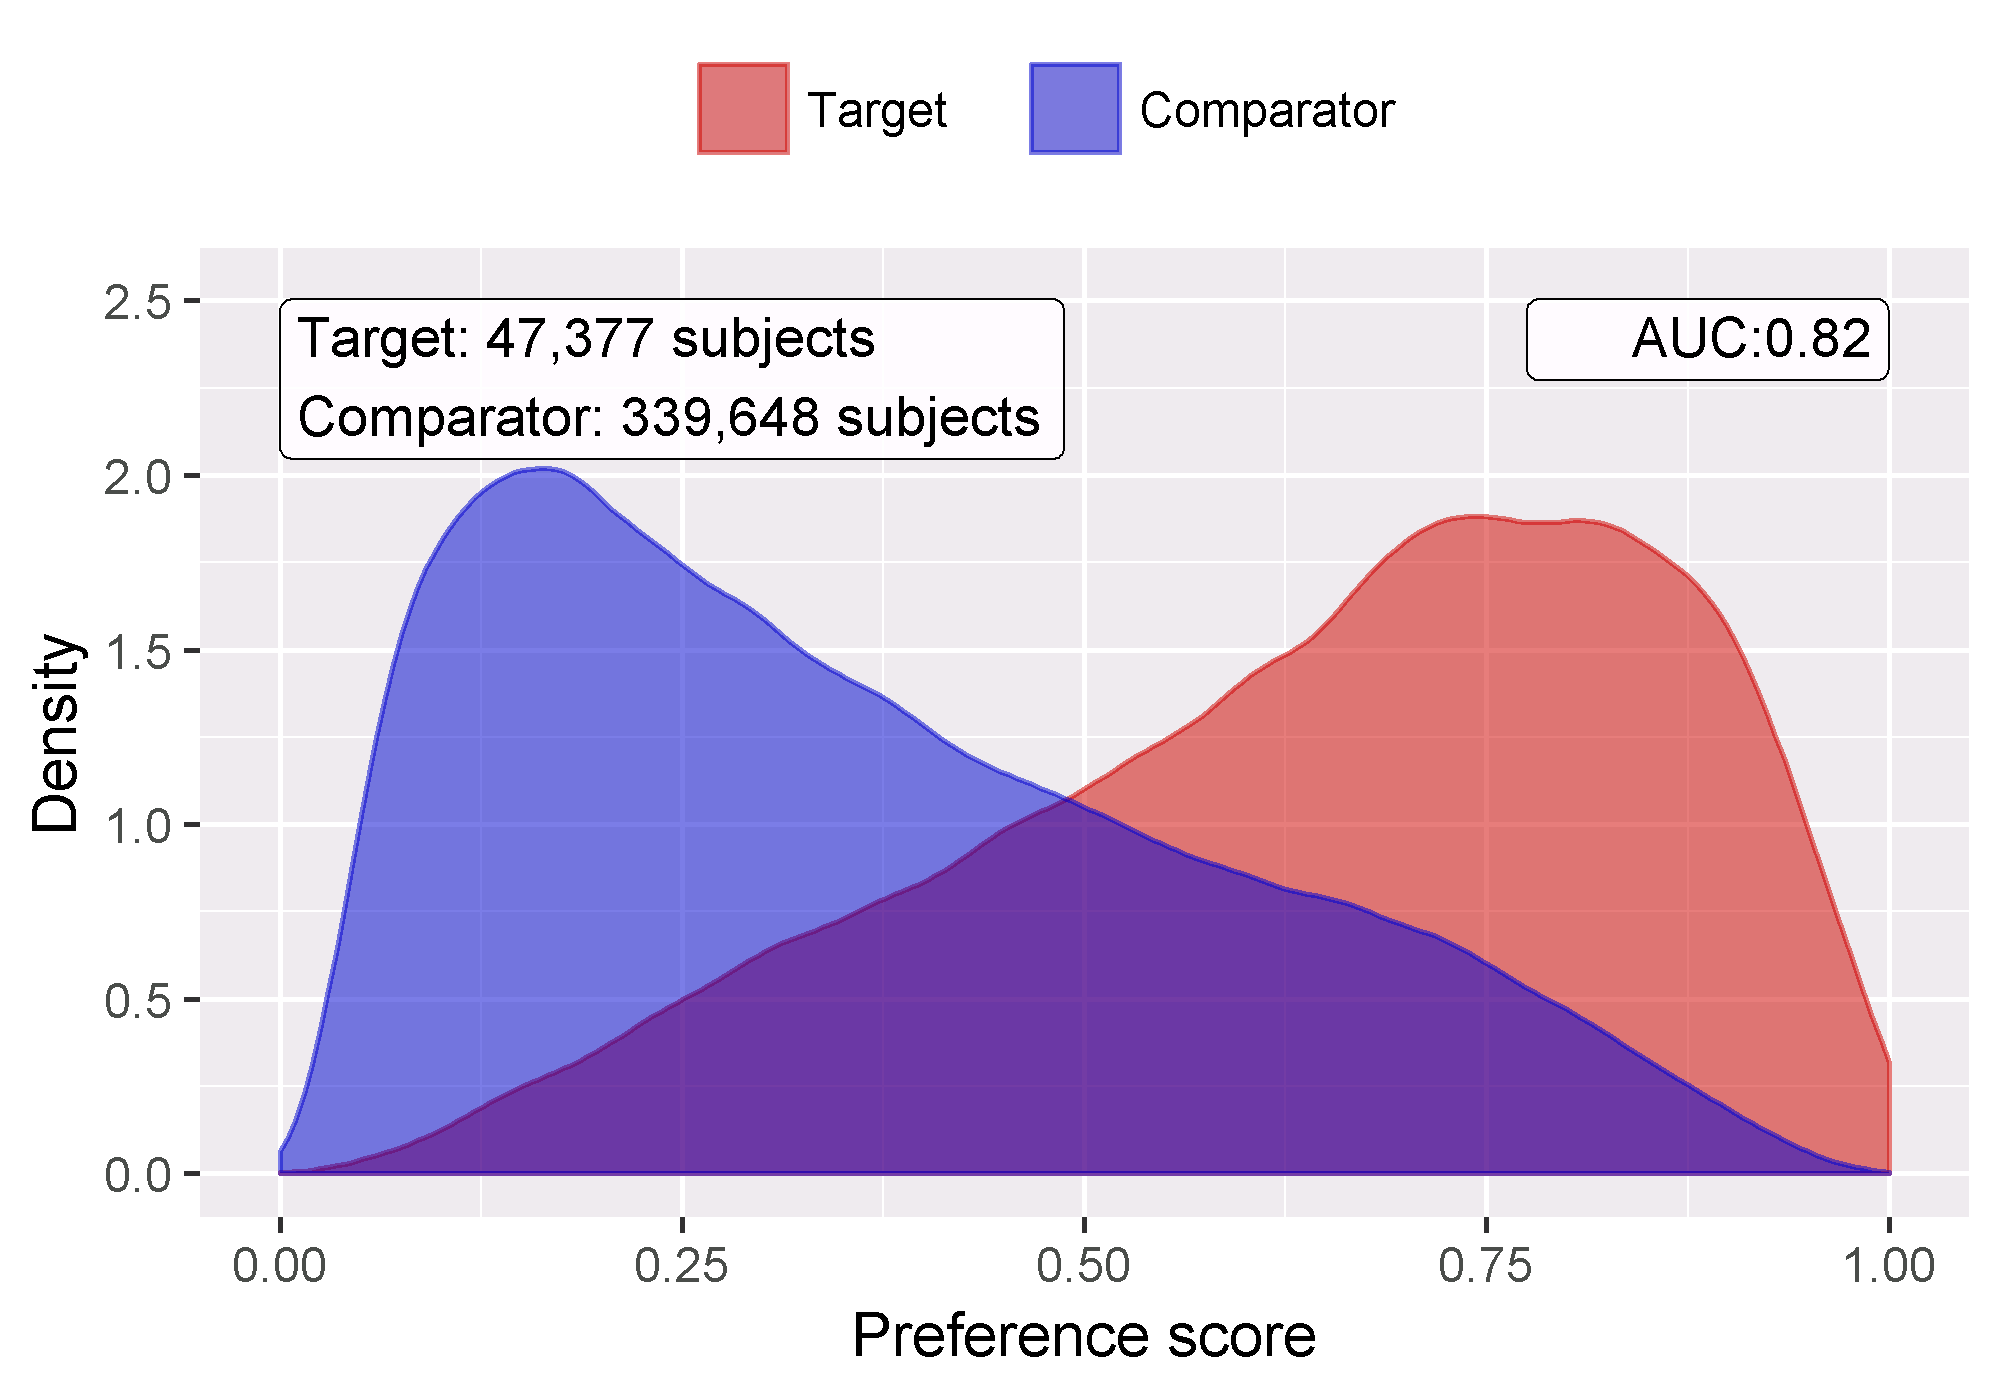
\includegraphics[width=0.8\linewidth]{images/MethodValidity/ps} 

}

\caption{Preference score distribution. The preference score is a transformation of the propensity score that adjusts for differences in the sizes of the two treatment groups. A higher overlap indicates subjects in the two groups were more similar in terms of their predicted probability of receiving one treatment over the other.}\label{fig:ps}
\end{figure}

Once we believe there is some hope of making the two groups comparable,
we need to evaluate whether we indeed succeed by examining a large
number of baseline characteristics after adjustment. Figure
\ref{fig:balanceScatterplot} shows the absolute standardized difference
of the mean between the two groups for a large number of covariates,
both before and after matching on the propensity score. A rule-of-thumb
that is often used is to consider any variabel with absolute
standardized difference of the mean \textless{} 0.1 to be in balance. We
see in Figure \ref{fig:balanceScatterplot} that many covariates show
imbalance before matching, but matching achieves balance on all
covariates.

\begin{figure}

{\centering 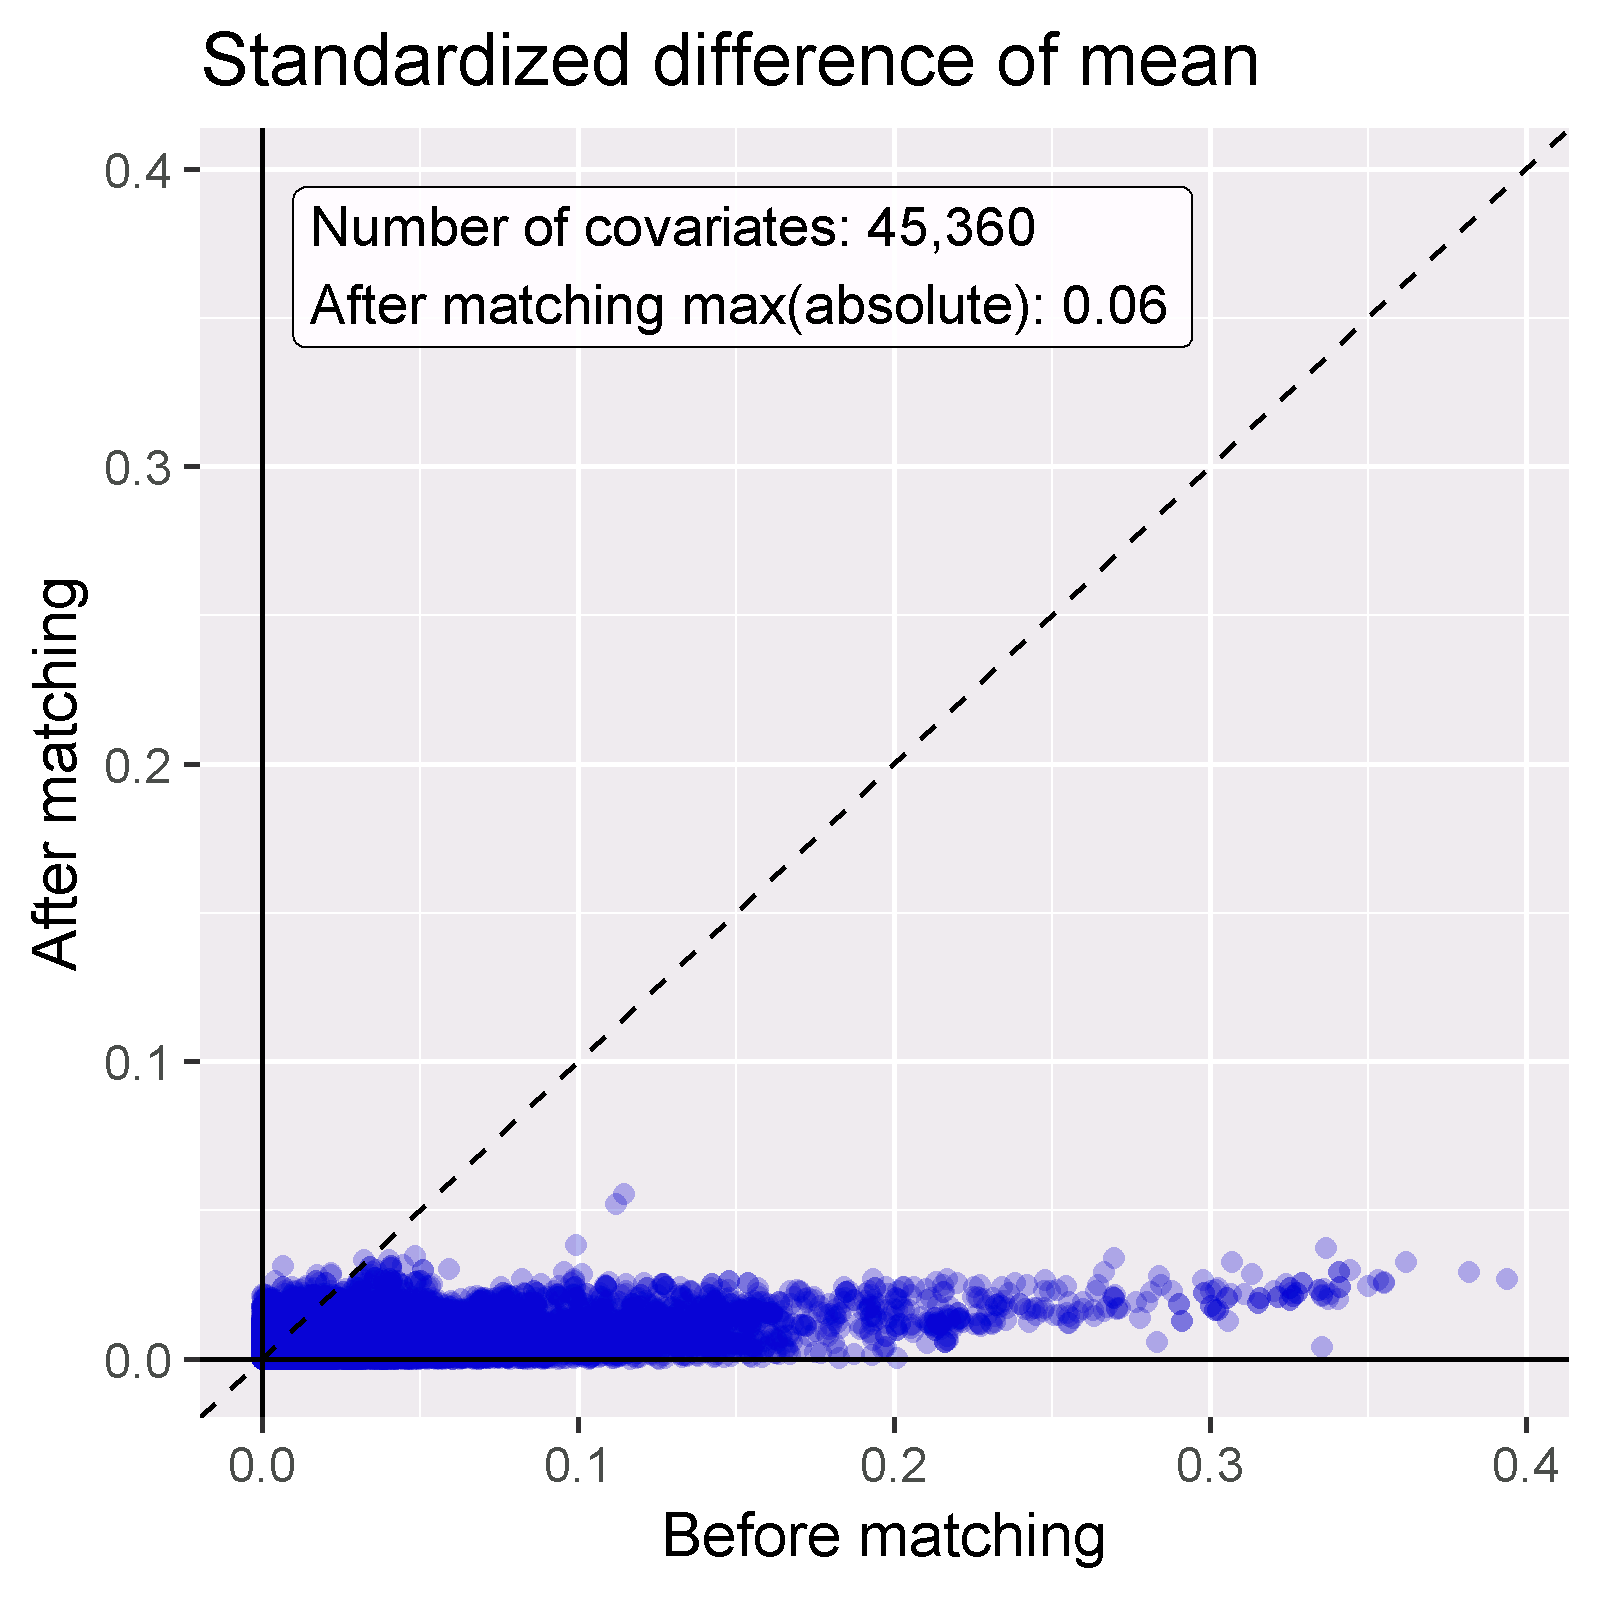
\includegraphics[width=0.6\linewidth]{images/MethodValidity/balanceScatterplot} 

}

\caption{Covariate balance before and after matching. Each dot represents the standardizes difference of means for a single covariate before and after matching on the propensity score. }\label{fig:balanceScatterplot}
\end{figure}

\subsection{Diagnostics for SCCS}\label{diagnostics-for-sccs}

One assumption in the self-controlled case series (SCCS) design is that
the end of observation is independent of the outcome. This assumption is
often violated in the case of serious, potentially lethal, events such
as myocardial infarction. We can evaluate whether the assumption holds
by generating the plot shown in Figure \ref{fig:timeToObsEnd}, which
shows a histograms of the time to obsevation period end for those that
are censored, and those that uncensored. In our data we consider those
whose observation period ends at the end date of data capture (the date
when observation stopped for the entire data base, for example the date
of extraction, or the study end date) to be uncensored, and all others
to be censored. In Figure \ref{fig:timeToObsEnd} we see only minor
differences between the two distributions, suggesting our assumptions
holds.

\begin{figure}

{\centering 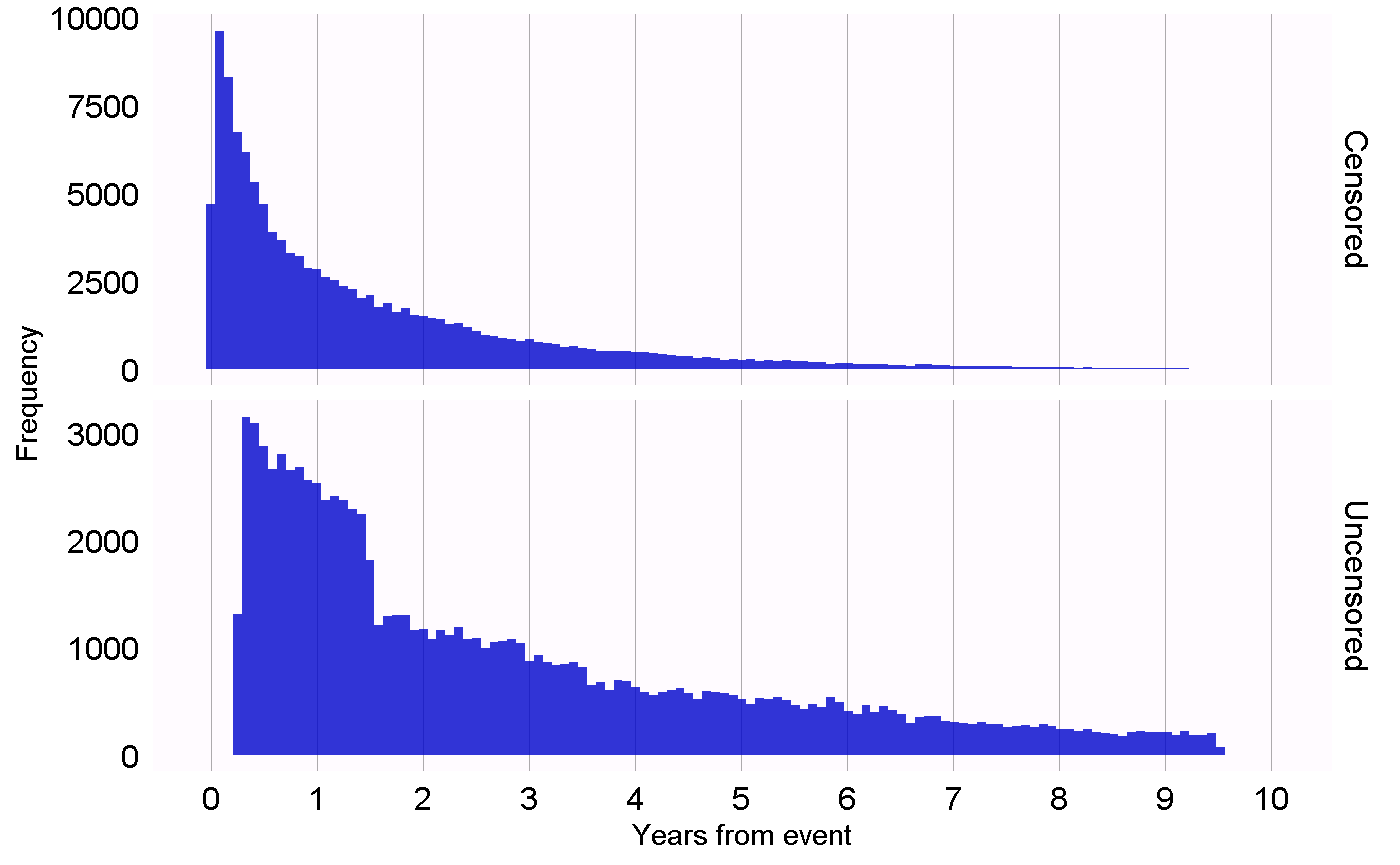
\includegraphics[width=1\linewidth]{images/MethodValidity/timeToObsEnd} 

}

\caption{Time to observation end for those that are censored, and those that uncensored.}\label{fig:timeToObsEnd}
\end{figure}

\section{Diagnostics for all
estimation}\label{diagnostics-for-all-estimation}

Some diagnostics are applicable for all population-level estimation
studies. These require the inclusion of control hypotheses, research
questions where the answer is already known. We can then evaluate
whether our design produces results in line with the truth. Controls can
be divided into negative controls and positive controls.

\subsection{Negative and positive
controls}\label{negative-and-positive-controls}

Negative controls are exposure-outcome pairs where one believes no
causal effect exists, and including negative controls or `falsification
endpoints' \citep{prased_2013} has been recommended as a means to detect
confounding \citep{lipsitch_2010}, selection bias and measurement error
\citep{arnold_2016}. For example, in one study \citep{zaadstra_2008}
investigating the relationship between childhood diseases and later
multiple sclerosis (MS), the authors include three negative controls
that are not believed to cause MS: a broken arm, concussion, and
tonsillectomy. Two of these three controls produce statistically
significant associations with MS, suggesting that the study may be
biased. We should select negative controls that are comparable to our
hypothesis of interest, which means we typically select exposure-outcome
pairs that either have the same exposure as the hypothesis of interest
(so-called `outcome controls') or the same outcome ('exposure controls).
In OHDSI we have developed a semi-automated procedure for selecting
negative controls \citep{voss_2016}. In brief, information from
literature, product labels, and spontaneous reporting is automatically
extracted and synthesized to produce a candidate list of outcomes with
no known links with any hypertension treatment. We rank-order this list
by prevalence in an observational database and manually review these in
order.

To understand the behavior of a method when the true relative risk is
smaller or greater than one requires the use of positive controls, where
the null is believed to not be true. Unfortunately, real positive
controls for observational research tend to be problematic for three
reasons. First, in most research contexts, for example when comparing
the effect of two treatments, there is a paucity of positive controls
relevant for that specific context. Second, even if positive controls
are available, the magnitude of the effect size may not be known with
great accuracy, and often depends on the population in which one
measures it. Third, when treatments are widely known to cause a
particular outcome, this shapes the behavior of physicians prescribing
the treatment, for example by taking actions to mitigate the risk of
unwanted outcomes, thereby rendering the positive controls useless as a
means for evaluation \citep{noren_2014}. In OHDSI we therefore use
synthetic positive controls \citep{schuemie_2018}, created by modifying
a negative control through injection of additional, simulated
occurrences of the outcome during the time at risk of the exposure. One
issue that stands important is the preservation of confounding. The
negative controls may show strong confounding, but if we inject
additional outcomes randomly, these new outcomes will not be confounded,
and we may therefore be optimistic in our evaluation of our capacity to
deal with confounding for positive controls. To preserve confounding, we
want the new outcomes to show similar associations with baseline
subject-specific covariates as the original outcomes. To achieve this,
we fit large-scale predictive models for each negative control using
\(L_1\) regularized survival regression \citep{suchard_2013}. We insert
new outcomes by drawing from the per-subject predicted probabilities
within the exposed population until we achieve the desired incidence
rate ratio. Figure \ref{fig:posControlSynth} depicts this process.

\begin{figure}

{\centering 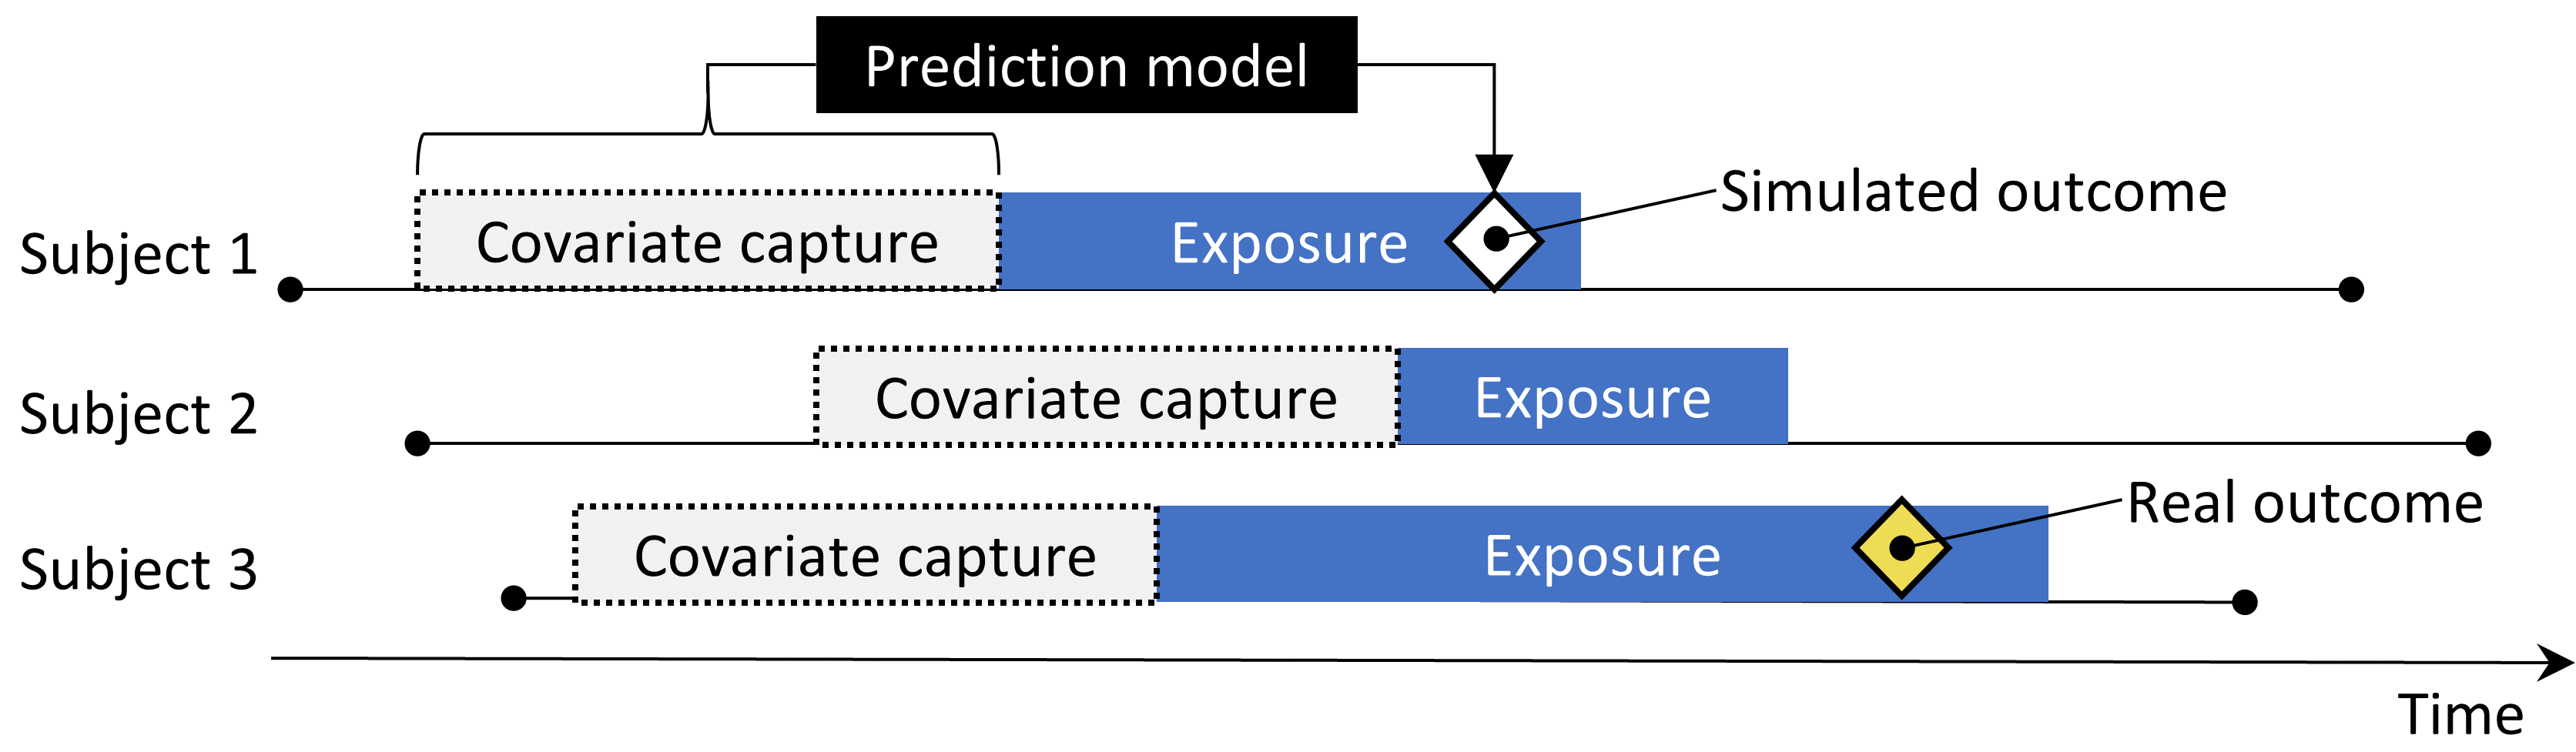
\includegraphics[width=0.9\linewidth]{images/MethodValidity/posControlSynth} 

}

\caption{Synthesizing positive controls from negative controls.}\label{fig:posControlSynth}
\end{figure}

\subsection{Metrics}\label{metrics}

Based on the estimates of a particular method for the negative and
positive controls, we can then understand the operating characteristic
by computing a range of metrics, for example:

\begin{itemize}
\tightlist
\item
  \textbf{Area Under the receiver operator Curve (AUC)}: the ability to
  discriminate between positive and negative controls.
\item
  \textbf{Coverage}: how often the true effect size is within the 95\%
  confidence interval.
\item
  \textbf{Mean precision}: precision is computed as 1 / (standard
  error)2, higher precision means narrower confidence intervals. We can
  use the geometric mean to account for the skewed distribution of the
  precision.
\item
  \textbf{Mean squared error (MSE)}: Mean squared error between the log
  of the effect size point-estimate and the log of the true effect size.
\item
  \textbf{Type 1 error}: For negative controls, how often was the null
  rejected (at alpha = 0.05). This is equivalent to the false positive
  rate and 1 - specificity.
\item
  \textbf{Type 2 error}: For positive controls, how often was the null
  not rejected (at alpha = 0.05). This is equivalent to the false
  negative rate and 1 - sensitivity.
\item
  \textbf{Non-estimable}: For how many of the controls was the method
  unable to produce an estimate? There can be various reasons why an
  estimate cannot be produced, for example because there were no
  subjects left after propensity score matching, or because no subjects
  remained having the outcome.
\end{itemize}

Depending on our use case, we can evaluate whether these operating
characterists are suitable for our goal. For example, if we wish to
perform signal detection, we may care about type I and type II error, or
if we are willing to modify our alpha threshold, we may inspect the AUC
instead.

\subsection{Empirical calibration}\label{empirical-calibration}

Often the type I error (at alpha = 0.05) is larger than 5\%, and the
coverage of the 95\% confidence interval is lower than 95\%. OHDSI has
developed processes for calibration p-values and confidence intervals to
restore these operating characteristics to nominal.

For p-value calibration \citep{schuemie_2014} we estimate the empirical
null distribution using the observed estimates for negative controls; We
fit a Gaussian probability distribution to the estimates, taking into
account the sampling error of each estimate. Using this null
distribution we then compute the calibrated p-value for the hypothesis
of interest, considering both random error and systematic error.

For confidence inteval calibration \citep{schuemie_2018} we estimate a
systematic error distribution, which we assume is Gaussian with a mean
and standard deviation linearly related to the logarithm of the true
effect size. Using the estimated distribution, we then generate
calibrated confidence intervals considering both random and systematic
error. Typically, but not necessarily, the calibrated confidence
interval is wider than the nominal confidence interval, reflecting the
problems unaccounted for in the standard procedure (such as unmeasured
confounding, selection bias and measurement error) but accounted for in
the calibration.

Both p-value calibration and confidence interval calibration are
implemented in the
\href{https://ohdsi.github.io/EmpiricalCalibration/}{EmpiricalCalibration}
package.

\subsection{Replication across sites}\label{replication-across-sites}

Another form of method validation can come from executing the study
across several different databases that possibly represent different
populations, different health care systems, and different data capture
processes. Prior research has shown that executing the same study design
across different databases can produce vastly different effect size
estimates \citep{madigan_2013}, suggesting the design does not
adequately address the different biases found in the different
databases. However, not observing heterogeneity of effects does not
guarantee an unbiased estimate. It is not unlikely that all databases
share a similar bias, and that all estimates are therefore consistently
wrong.

\subsection{Sensitivity analyses}\label{sensitivity-analyses}

When designing a study there are often design choices that are
uncertain. For example, should propensity score matchign of
stratification be used? If stratification is used, how many strata? What
is the appropriate time-at-risk? When faced with such uncertainty, one
solution is to evaluate various options, and observe the sensitivity of
the results to the design choice. If the estimate remains the same under
various options, we can say the study is robust to the uncertainty.

This definition of sensitivity analysis should not be confused with the
definitions used by others such as \citet{rosenbaum_2005}, who define
sensitivity analysis to `appraise how the conclusions of a study might
be altered by hidden biases of various magnitudes'.

\section{Diagnostics for all
prediction}\label{diagnostics-for-all-prediction}

Todo

\section{Method validation in
practice}\label{method-validation-in-practice}

Example: risk of angioedema and AMI in new users of ACE inhibitors
compared to new users of thiazide and thiazide-like diuretics

How to select negative controls using ATLAS

\begin{itemize}
\tightlist
\item
  Create a concept set containing both target and comparator exposure
  concepts.
\item
  Go to the `Explore evidence' tab and click `Generate'
\item
  Manually review negative controls, considering
\item
  Does the drug not cause the outcome?
\item
  Does the drug not prevent / treat the outcome?
\item
  Does the negative control appear in the data?
\end{itemize}

Include negative and positive controls.

Compute metrics

\begin{itemize}
\tightlist
\item
  Need to add functions to MethodEvaluation
\end{itemize}

Generate calibration plots

Calibrate CI and p-value

\begin{itemize}
\tightlist
\item
  Use EmpiricalCalibration package
\end{itemize}

\section{Advanced: OHDSI Methods
Benchmark}\label{advanced-ohdsi-methods-benchmark}

Todo: add text on OHDSI Methods Benchmark

\part{OHDSI Studies}\label{part-ohdsi-studies}

\chapter{Study steps}\label{StudySteps}

Writing the protocol, OHDSI style:
\url{http://www.ohdsi.org/web/wiki/lib/exe/fetch.php?media=projects:workgroups:wg_study_protocols_eastern_hemisphere.pptx}

Study reproducibility (Martijn has some slides that might help:
\url{http://www.ohdsi.org/web/wiki/lib/exe/fetch.php?media=projects:workgroups:wg_study_reproducability.pptx}
)

\chapter{OHDSI Network Research}\label{NetworkResearch}

Contributors: Greg Klebanov, Vojtech Huser, list others

What is OHDSI Network?

\begin{itemize}
\tightlist
\item
  OHDSI Community and Network Research
\item
  International Open Science Networks
\item
  OHDSI US
\item
  OHDSI EU and EHDEN
\item
  OHDSI APAC
\end{itemize}

OHDSI Network Study Process

\begin{itemize}
\tightlist
\item
  Goals
\item
  Workflow Overview
\item
  Structure of Studies
\item
  Protocol and IRB issues
\item
  Existing framework (de-identified {[}time shifted{]} OMOP dataset
  under existing IRB protocol
\item
  Overcoming Network Study Challenges
\item
  Data Privacy, Security and Compliance
\item
  Data Quality
\item
  Running OHDSI Methods in Isolated Environment
\item
  OMOP CDM Versioning
\end{itemize}

Tools, Platforms and Study Automation * OHDSI Methods support for
Network Studies * LEGEND (should we have it here?) * OHDSI ARACHNE
Network Platform

Opportunities, future trends and Roadmap

\section{OHDSI Network Study
Examples}\label{ohdsi-network-study-examples}

\subsection{Endometriosis study}\label{endometriosis-study}

An endometriosis characterization study (available at
\url{https://github.com/molliemckillop/Endometriosis-Phenotype-Characterization})
works with two cohorts. They are defined in cohorts.csv file (see here
\url{https://github.com/molliemckillop/Endometriosis-Phenotype-Characterization/blob/master/inst/settings/cohorts.csv}).

After creating a cohort table, it is populated by executing this command
here by infering a name of a `.sql' file from the previously defined
cohort file. A createCohorts function is executed next. (see
\url{https://github.com/molliemckillop/Endometriosis-Phenotype-Characterization/blob/master/R/createCohorts.R}).
An SQL file that is generated by Atlas populates the cohort table with
specific person\_ids that fulfill the cohort definition.

\section{Excercises}\label{excercises-2}

\subsection{Defining a cohort}\label{defining-a-cohort}

Q: Study the code for the x study and determine whether the cohort
definition is available on the public OHDSI server. It if it, what is
the cohort ID there?

A:

\appendix


\chapter{Glossary}\label{Glossary}

Cohort A cohort is a list of person\_ids with start and end date. It is
stored in a study specific cohort table or a CDM specified cohort table
can also be used. Cohort can be represented as .json file. It is used
for import and export but not during an analysis. OHDSI tools use SQL so
Atlas also generates a .sql file that creates the cohort during
analysis.

Parametized SQL code An SQL code that allows for use of parameters.
Parameters are prefixed with @. Such code has to be ``rendered''.
Synonym: OHDSI SQL code.

\chapter{Cohort definitions}\label{CohortDefinitions}

This Appendix contains cohort definitions used throughout the book.

\section{ACE inhibitors}\label{AceInhibitors}

\textbf{Initial Event Cohort}

People having any of the following:

\begin{itemize}
\tightlist
\item
  a drug exposure of \emph{ACE inhibitors} (Table
  \ref{tab:aceInhibitors}) for the first time in the person's history
\end{itemize}

with continuous observation of at least 365 days prior and 0 days after
event index date, and limit initial events to: all events per person.

Limit qualifying cohort to: all events per person.

\textbf{End Date Strategy}

Custom Drug Era Exit Criteria This strategy creates a drug era from the
codes found in the specified concept set. If the index event is found
within an era, the cohort end date will use the era's end date.
Otherwise, it will use the observation period end date that contains the
index event.

Use the era end date of \emph{ACE inhibitors} (Table
\ref{tab:aceInhibitors})

\begin{itemize}
\tightlist
\item
  allowing 30 days between exposures
\item
  adding 0 days after exposure end
\end{itemize}

\textbf{Cohort Collapse Strategy}

Collapse cohort by era with a gap size of 30 days.

\textbf{Concept Set Definitions}

\begin{longtable}[]{@{}lllll@{}}
\caption{\label{tab:aceInhibitors} ACE inhibitors}\tabularnewline
\toprule
Concept Id & Concept Name & Excluded & Descendants &
Mapped\tabularnewline
\midrule
\endfirsthead
\toprule
Concept Id & Concept Name & Excluded & Descendants &
Mapped\tabularnewline
\midrule
\endhead
1308216 & Lisinopril & NO & YES & NO\tabularnewline
1310756 & moexipril & NO & YES & NO\tabularnewline
1331235 & quinapril & NO & YES & NO\tabularnewline
1334456 & Ramipril & NO & YES & NO\tabularnewline
1335471 & benazepril & NO & YES & NO\tabularnewline
1340128 & Captopril & NO & YES & NO\tabularnewline
1341927 & Enalapril & NO & YES & NO\tabularnewline
1342439 & trandolapril & NO & YES & NO\tabularnewline
1363749 & Fosinopril & NO & YES & NO\tabularnewline
1373225 & Perindopril & NO & YES & NO\tabularnewline
\bottomrule
\end{longtable}

\section{Angioedema}\label{Angioedema}

\textbf{Initial Event Cohort}

People having any of the following:

\begin{itemize}
\tightlist
\item
  a condition occurrence of \emph{Angioedema} (Table
  \ref{tab:angioedema})
\end{itemize}

with continuous observation of at least 0 days prior and 0 days after
event index date, and limit initial events to: all events per person.

For people matching the Primary Events, include: Having any of the
following criteria:

\begin{itemize}
\tightlist
\item
  at least 1 occurrences of a visit occurrence of \emph{Inpatient or ER
  visit} (Table \ref{tab:inpatientOrEr}) where event starts between all
  days Before and 0 days After index start date and event ends between 0
  days Before and all days After index start date
\end{itemize}

Limit cohort of initial events to: all events per person.

Limit qualifying cohort to: all events per person.

\textbf{End Date Strategy}

This cohort defintion end date will be the index event's start date plus
7 days

\textbf{Cohort Collapse Strategy}

Collapse cohort by era with a gap size of 30 days.

\textbf{Concept Set Definitions}

\begin{longtable}[]{@{}lllll@{}}
\caption{\label{tab:angioedema} Angioedema}\tabularnewline
\toprule
Concept Id & Concept Name & Excluded & Descendants &
Mapped\tabularnewline
\midrule
\endfirsthead
\toprule
Concept Id & Concept Name & Excluded & Descendants &
Mapped\tabularnewline
\midrule
\endhead
432791 & Angioedema & NO & YES & NO\tabularnewline
\bottomrule
\end{longtable}

\begin{longtable}[]{@{}lllll@{}}
\caption{\label{tab:inpatientOrEr} Inpatient or ER visit}\tabularnewline
\toprule
Concept Id & Concept Name & Excluded & Descendants &
Mapped\tabularnewline
\midrule
\endfirsthead
\toprule
Concept Id & Concept Name & Excluded & Descendants &
Mapped\tabularnewline
\midrule
\endhead
262 & Emergency Room and Inpatient Visit & NO & YES & NO\tabularnewline
9201 & Inpatient Visit & NO & YES & NO\tabularnewline
9203 & Emergency Room Visit & NO & YES & NO\tabularnewline
\bottomrule
\end{longtable}

\bibliography{book.bib,packages.bib}


\end{document}
